\documentclass[11pt]{opticajnl}
\journal{opticajournal} % use for journal or Optica Open submissions

\usepackage[utf8]{inputenc}
\usepackage[T1]{fontenc} % Añadir esta línea para mejorar el manejo de caracteres especiales

\usepackage{etoolbox}

\makeatletter
\AtBeginEnvironment{minted}{\dontdofcolorbox}
\def\dontdofcolorbox{\renewcommand\fcolorbox[4][]{##4}}
\makeatother
% See template introduction for guidance on setting shortarticle option
\setboolean{shortarticle}{true}
% true = letter/tutorial
% false = research/review article

% ONLY applicable for journal submission shortarticle types:
% When \setboolean{shortarticle}{true}
% then \setboolean{memo}{true} will print "Memorandum" on title page header
% Otherwise header will remain as "Letter"
% \setboolean{memo}{true}
\usepackage{lineno}
\usepackage{listings}
\usepackage{color}  % Para colorear el código
\usepackage[outputdir=build]{minted}

\definecolor{dkgreen}{rgb}{0,0.6,0}
\definecolor{gray}{rgb}{0.5,0.5,0.5}
\definecolor{mauve}{rgb}{0.58,0,0.82}
\lstset{language=SQL,
  basicstyle={\small\ttfamily},
  belowskip=3mm,
  breakatwhitespace=true,
  breaklines=true,
  classoffset=0,
  columns=flexible,
  commentstyle=\color{dkgreen},
  framexleftmargin=0.25em,
  frameshape={}{yy}{}{}, %To remove to vertical lines on left, set `frameshape={}{}{}{}`
  keywordstyle=\color{blue},
  numbers=none, %If you want line numbers, set `numbers=left`
  numberstyle=\tiny\color{gray},
  showstringspaces=false,
  stringstyle=\color{dkgreen},
  tabsize=3,
  xleftmargin =1em, 
  literate={'}{{\texttt{'}}}1
  		   {"}{{\texttt{"}}}1
}


\lstdefinestyle{terminal}{
  backgroundcolor=\color{white},   % Fondo blanco
  basicstyle=\color{black}\ttfamily, % Texto negro en fuente monoespaciada
  keywordstyle=\color{black}\bfseries, % Palabras clave en azul y negrita
  commentstyle=\color{black}\ttfamily, % Comentarios en verde
  stringstyle=\color{black}\ttfamily, % Cadenas en rojo
  morekeywords={sudo, apt-get, install, cd, ls, mkdir, rm, rmdir, cp, mv, echo, cat, nano, vim, grep, find, chmod, chown, systemctl, service, update, upgrade, reboot, shutdown, exit}, % Comandos comunes de terminal
  breaklines=true, % Permitir saltos de línea
  frame=single, % Marco alrededor del código
  framerule=0.5pt, % Grosor del marco
  rulecolor=\color{gray}, % Color del marco
  xleftmargin=0.05\textwidth, % Margen izquierdo
  xrightmargin=0.05\textwidth, % Margen derecho
  aboveskip=1em, % Espacio antes del bloque de código
  belowskip=1em % Espacio después del bloque de código
}

% Definir el lenguaje Cypher
\lstdefinelanguage{Cypher}{
  keywords={
    MATCH, RETURN, WHERE, CREATE, DELETE, SET, MERGE, 
    WITH, UNION, UNION ALL, LOAD CSV, USING, INDEX,
    START, FOREACH, ON, WHEN, CASE, THEN, ELSE, END,
    SKIP, LIMIT, ORDER BY, DESC, ASC, IN, AND, OR, NOT,
    CONTAINS, DISTINCT, OPTIONAL, DETACH, EXISTS,
    CONSTRAINT, ASSERT, UNIQUE, DROP, REMOVE, ORDER, BY
  },
  sensitive=true,
  comment=[l]//,
  morecomment=[s]{/*}{*/},
  morestring=[b]',
  morestring=[b]"
}


%\linenumbers % Turn off line numbering for Optica Open preprint submissions.

\title{Trabajo de prácticas BDGE}

\author[1,2,3]{Luis Ardévol Mesa, Miguel Mato Martínez}


\begin{abstract}
Usando una conjunto de datos de partidos de tenis, se usarán distintos tipos de base de datos para realizar consultas acerca de los mismos. En concreto, se tratarán bases de datos relaciones y con datos agregados en PostgreSQL, bases de datos distribuidas con SQL usando CITUS Data, y dos tipos de bases de datos noSQL: documentales con MongoDB y en grafo con Neo4j.
\end{abstract}

\setboolean{displaycopyright}{false} % Do not include copyright or licensing information in submission.

\begin{document}

\maketitle


\section{Bases de datos relacionales (PostgreSQL)}

\begin{figure}[H]
  \centering
  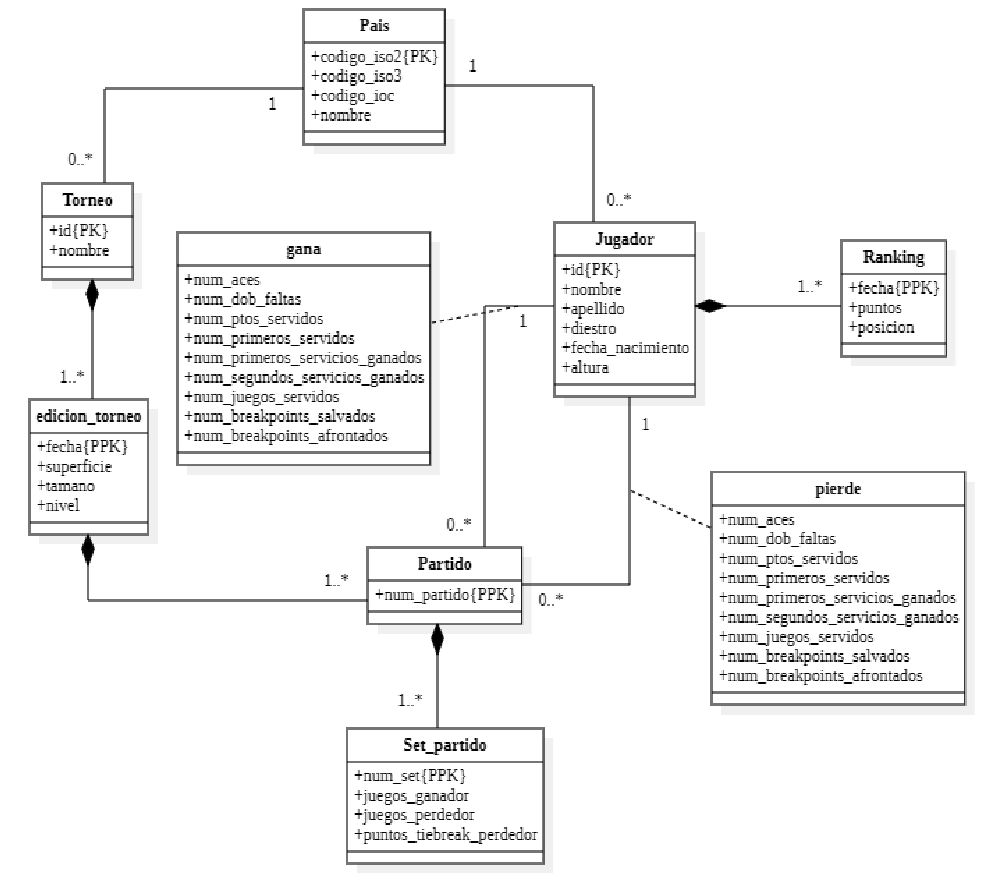
\includegraphics[width=0.7\textwidth]{fotos/esquema.png}
  \caption{Esquema de la base de datos de partidos de tenis.}
  \label{fig:schbd}
\end{figure}

En la figura \ref{fig:schbd} se muestra el esquema de la base de datos de partidos de tenis. Comenzaremos explicando este esquema de forma breve, pero haciendo especial hincapié en las relaciones entre las distintas tablas, ya que esto ayudará a comprender mejor las condiciones de \textit{join} a usar en las consultas que usen este esquema. Destacamos que no se hará uso de la tabla \texttt{ranking}, por lo que no se comentará en el siguiente análisis. \\

La tabla \texttt{pais} contiene la información relativa a países, y se usará tanto para mostrar el país dónde se celebra un torneo como para referenciar el país de procedencia de un jugador; su clave primaria es \texttt{codigo\_iso2}. La tabla \texttt{jugador} contiene la información de los jugadores, y su clave primaria es el \texttt{id} de cada jugador; el atributo \texttt{pais} referencia a \texttt{pais(codigo\_iso2)}. La tabla \texttt{torneo} contiene la información de los torneos; su clave primaria es el \texttt{id} de cada torneo y el atributo \texttt{pais} referencia a \texttt{pais(codigo\_iso2)}. La tabla \texttt{edicion\_torneo} contiene la información de las ediciones de los torneos; su clave primaria es una combinación de los atributos \texttt{torneo} y \texttt{fecha}, donde el atributo \texttt{torneo} es una referencia a \texttt{torneo(id)}. La tabla \texttt{partido} contiene la información de los partidos disputados; su clave primaria es la combinación de los atributos \texttt{torneo}, \texttt{fecha} y \texttt{num\_partido}, y tiene una clave foránea compuesta por los atributos \texttt{torneo} y \texttt{fecha}, que referencia a la clave primaria de \texttt{edicion\_torneo}, \texttt{edicion\_torneo(torneo, fecha)}. Además, los atributos \texttt{ganador} y \texttt{perdedor} son los \texttt{id} de los jugadores, por lo que puede enlazarse esta tabla con la de \texttt{jugador} mediante \texttt{jugador(id)}. Por último, la tabla \texttt{sets\_partido} contiene la información de los sets de los partidos; su clave primaria es la combinación de los atributos \texttt{torneo}, \texttt{fecha}, \texttt{num\_partido} y \texttt{num\_set}, y tiene una clave foránea compuesta por los atributos \texttt{torneo}, \texttt{fecha} y \texttt{num\_partido}, que referencia a la clave primaria de \texttt{partido}, \texttt{partido(torneo, fecha, num\_partido)}. \\

Tras ver cómo se estructura la base de datos a usar, creamos la base de datos en PostgreSQL y cargamos los datos en ella. La estructura relacional se proporciona en el archivo \texttt{schema.sql}, y los datos en los archivos \texttt{pais.csv}, \texttt{jugador.csv}, \texttt{torneo.csv}, \texttt{edicion\_torneo.csv}, \texttt{partido.csv}, \texttt{sets\_partido.csv} y \texttt{ranking.csv}. Una vez creada la base de datos \texttt{tenis}, ejecutamos el archivo \texttt{schema.sql} con la definición de los esquemas de las tablas mediante el siguiente comando en la terminal:

\begin{lstlisting}[style=terminal]
psql -U alumnogreibd -d tenis -f /home/alumnogreibd/BDGE/datos/datos_tenis/schema.sql
\end{lstlisting}

Ahora, con los esquemas definidos (pero vacíos), cargamos los datos a partir de los archivos \texttt{.csv} con los siguientes comandos en terminal (es importante seguir el orden de carga de los datos debido a las dependencias entre las tablas):

\begin{lstlisting}[style=terminal]
psql -U alumnogreibd -d tenis -c "\copy pais from /home/alumnogreibd/BDGE/datos/datos_tenis/pais.csv csv"
psql -U alumnogreibd -d tenis -c "\copy jugador from /home/alumnogreibd/BDGE/datos/datos_tenis/jugador.csv csv"
psql -U alumnogreibd -d tenis -c "\copy torneo from /home/alumnogreibd/BDGE/datos/datos_tenis/torneo.csv csv"
psql -U alumnogreibd -d tenis -c "\copy edicion_torneo from /home/alumnogreibd/BDGE/datos/datos_tenis/edicion_torneo.csv csv"
psql -U alumnogreibd -d tenis -c "\copy partido from /home/alumnogreibd/BDGE/datos/datos_tenis/partido.csv csv"
psql -U alumnogreibd -d tenis -c "\copy sets_partido from /home/alumnogreibd/BDGE/datos/datos_tenis/sets_partido.csv csv"
psql -U alumnogreibd -d tenis -c "\copy ranking from /home/alumnogreibd/BDGE/datos/datos_tenis/ranking.csv csv"
\end{lstlisting}

Este orden es lógico por las dependencias entre tablas que comentamos anteriormente: \texttt{sets\_partido} referencia a \texttt{partido}, por lo que es necesario cargar primero los datos de \texttt{partido} para poder cargar los de \texttt{sets\_partido}. Este razonamiento aplica al resto de tablas: \texttt{partido} referencia a \texttt{edicion\_torneo}, que referencia a \texttt{torneo}, que a su vez referencia a \texttt{pais}, que es referenciado por \texttt{jugador}. \\

En las siguientes consultas, los \textit{join} se harán mediante \textit{theta join} (\textit{inner} por defecto). En caso de que se quiera hacer otro tipo de \textit{join}, se especificará de forma clara en la consulta. Esto considera el producto cartesiano de las tablas a unir y selecciona solo las tuplas que verifiquen el predicado (la condición o condiciones de \textit{join}). Estos \textit{join} se harán de forma general de forma implícita en la claúsula \texttt{where}, siguiendo los atributos referenciados entre las tablas. El \texttt{where} hace una selección de tuplas (filas) que cumplen el predicado o los predicados mencionados. Teniendo esto muy presente, abusaremos un poco del lenguaje para ser más concisos y frases como: ``seleccionamos solo las tuplas en las que un jugador concreto es el ganador del partido'', reformularemos como ``seleccionamos los partidos que ganó un jugador concreto''. \\


\subsubsection{Muestra todos los ganadores del torneo ``Wimbledon'' (Nombre, apellidos y año). Ordena el resultado por año.}

Para esta consulta necesitamos la información de los jugadores, los partidos y los torneos, por lo que comenzamos en el \texttt{from} con el producto cartesiano de las tablas \texttt{jugador}, \texttt{partido} y \texttt{torneo} (especificando un alias para cada una de ellas). A continuación, especificamos las condiciones de \textit{join} en el \texttt{where}, así como otras condiciones de selección: 
\begin{itemize}
\item Condiciones de \textit{join}:
\begin{itemize}
\item El predicado \texttt{j.id = p.ganador} sirve para unir la tabla \texttt{jugador} con la tabla \texttt{partido} mediante el atributo \texttt{id} de la tabla \texttt{jugador} y el atributo \texttt{ganador} de la tabla \texttt{partido}, haciendo una selección únicamente de las tuplas que cumplan esta condición. Esto nos permite, para cada jugador, seleccionar solo los partidos en los que ha ganado.
\item El predicado \texttt{t.id = p.torneo} sirve para unir la tabla \texttt{torneo} con la tabla \texttt{partido} mediante el atributo \texttt{id} de la tabla \texttt{torneo} y el atributo \texttt{torneo} de la tabla \texttt{partido}, haciendo una selección únicamente de las tuplas que cumplan esta condición. Esto nos permite seleccionar solo los partidos que se han jugado en un torneo concreto.
\end{itemize}
\item Condiciones de selección:
\begin{itemize}
\item La condición \texttt{t.nombre = `Wimbledon'} selecciona solo el torneo cuyo nombre es ``Wimbledon''. Al hacer el \textit{join} con la tabla \texttt{torneo}, estamos seleccionando solo los partidos que se han jugado en el torneo ``Wimbledon''.
\item La condición \texttt{p.ronda = `F'} selecciona solo los partidos que han sido finales.
\end{itemize}
\end{itemize}

Tras seleccionar las tuplas que nos interesan, usamos el \texttt{select} para obtener la proyección de las filas que nos interesan: en esta caso, nos quedamos con los atributos \texttt{nombre} y \texttt{apellido} de la tabla \texttt{jugador} y el año de la fecha del partido, que denotaremos por el alias ``ano''. Como \texttt{p.fecha} es del tipo \texttt{date}, este último atributo lo obtenemos mediante la función \texttt{extract()}, especificando que solo queremos el año de ese atributo (\texttt{year from p.fecha}). Tras esto, ordenamos el resultado por año con \texttt{order by ano}; el orden por defecto es ascendente. El código de la consulta se muestra a continuación, y el resultado se pueden ver en la figura \ref{fig:q1_rel}.

\begin{minted}[frame=single, fontsize=\footnotesize]{sql}
select j.nombre, j.apellido, extract(year from p.fecha) as ano
from jugador j, partido p, torneo t
where j.id = p.ganador 
  and t.id = p.torneo 
  and t.nombre = 'Wimbledon' 
  and p.ronda = 'F'
order by ano
\end{minted}

\begin{figure}[H]
\centering
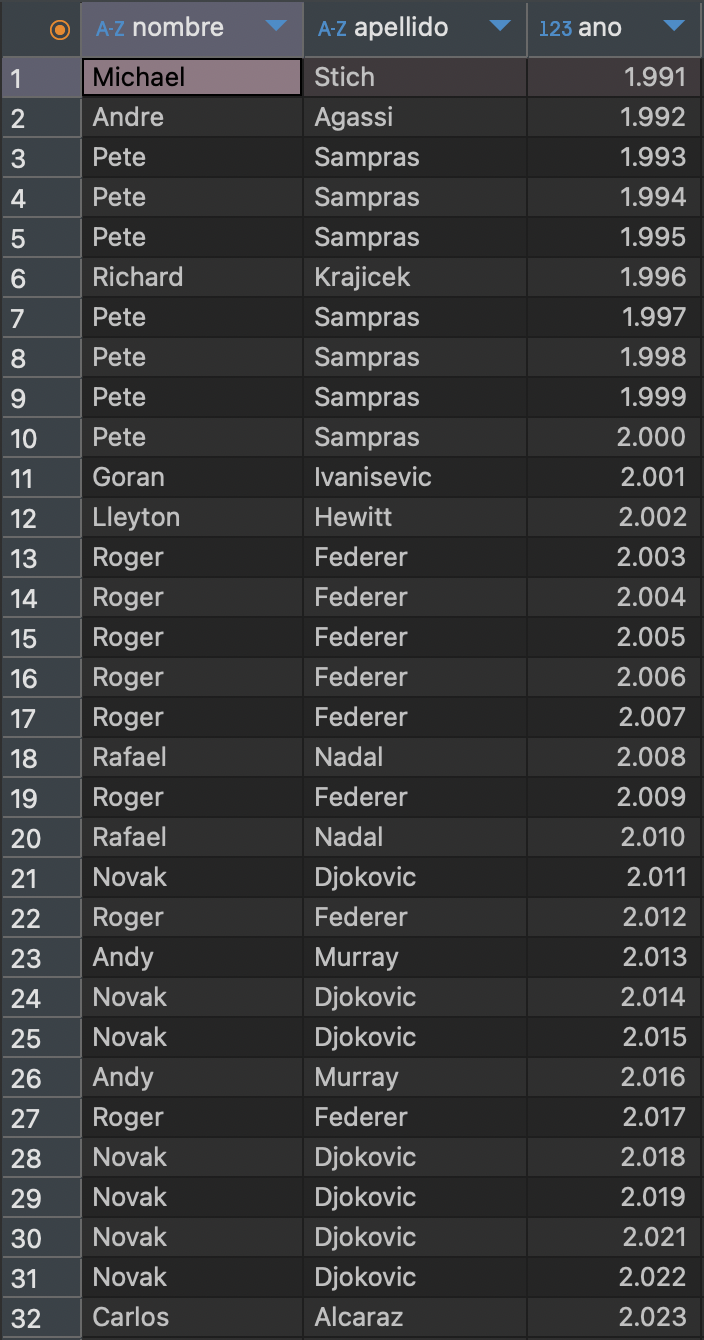
\includegraphics[height=0.4\textheight]{fotos/q1_rel.png}
\caption{Modelo relacional Postgresql, consulta 1.}
\label{fig:q1_rel}
\end{figure}



\subsubsection{Muestra los años en los que Roger Federer ganó algún torneo de nivel Gran Slam (G) o Master 1000 (M). Para cada año, muestra el número de torneos y lista sus nombres (ordenados por la fecha de celebración). Ordena el resultado por el año}

Para esta consulta necesitamos información de los jugadores, los partidos, los torneos y las ediciones de los torneos. Comenzamos en el \texttt{from} con el producto cartesiano de las tablas \texttt{jugador}, \texttt{partido}, \texttt{torneo} y \texttt{edicion\_torneo} (especificando un alias para cada una de ellas). A continuación, especificamos las condiciones de \textit{join} en el \texttt{where}, así como otras condiciones de selección:
\begin{itemize}
\item Condiciones de \textit{join} que, en global, nos permitirán seleccionar las tuplas de un jugador específico que ganó un torneo específico en un año específico:
\begin{itemize}
\item El predicado \texttt{j.id = p.ganador} sirve para unir la tabla \texttt{jugador} con la tabla \texttt{partido} mediante el atributo \texttt{id} de la tabla \texttt{jugador} y el atributo \texttt{ganador} de la tabla \texttt{partido}, haciendo una selección únicamente de las tuplas que cumplan esta condición. Esto nos permite, para cada jugador, seleccionar solo los partidos en los que ha ganado.
\item El predicado \texttt{t.id = p.torneo} sirve para unir la tabla \texttt{torneo} con la tabla \texttt{partido} mediante el atributo \texttt{id} de la tabla \texttt{torneo} y el atributo \texttt{torneo} de la tabla \texttt{partido}, haciendo una selección únicamente de las tuplas que cumplan esta condición. Esto nos permite seleccionar solo los partidos que se han jugado en un torneo concreto.
\item El predicado \texttt{t.id = et.torneo} sirve para unir la tabla \texttt{torneo} con la tabla \texttt{edicion\_torneo} mediante el atributo \texttt{id} de la tabla \texttt{torneo} y el atributo \texttt{torneo} de la tabla \texttt{edicion\_torneo}, haciendo una selección únicamente de las tuplas que cumplan esta condición. Esto nos permite seleccionar ediciones de torneos concretos.
\item El predicado \texttt{p.fecha = et.fecha} sirve para unir la tabla \texttt{partido} con la tabla \texttt{edicion\_torneo} mediante el atributo \texttt{fecha} de la tabla \texttt{partido} y el atributo \texttt{fecha} de la tabla \texttt{edicion\_torneo}, haciendo una selección únicamente de las tuplas que cumplan esta condición. Esto nos permite seleccionar solo los partidos que se han jugado en una edición concreta de un torneo (concreto, por la condición anterior).
\end{itemize}
\item Estamos interesados específicamente en torneos de nivel Gran Slam (G) o Master 1000 (M) y en las finales ganadas por Roger Federer (lo que indica que ganó el torneo) durante varios años (es decir, varias ediciones de torneos). Por tanto, las condiciones de selección son:
\begin{itemize}
\item El predicado \texttt{p.ronda = 'F'} selecciona solo los partidos que han sido finales.
\item El predicado \texttt{j.nombre = 'Roger' and j.apellido = 'Federer'} selecciona solo los partidos en los que ha ganado ``Roger Federer''.
\item El predicado \texttt{et.nivel in ('G', 'M')} selecciona solo los torneos de nivel Gran Slam (G) o Master 1000 (M).
\end{itemize}
\end{itemize}

Con el \texttt{group by} agrupamos los resultados por el año en que se celebraron los torneos, para su posterior concatenación. Por último, obtenemos la proyección de los atributos que nos interesan: el año, que lo obtenemos extrayendo el año de la fecha de celebración del partido; el número de torneos ganados, que lo obtenemos contando el número de torneos distintos (usamos el \texttt{id} del torneo para diferenciar) en el resultado agrupado por año (\texttt{count(distinct t.id)}). Como última proyección, obtenemos una concantenación (con \texttt{string\_agg()}) de esos torneos, separados por comas y ordenados por fecha de celebración de esa edición, en orden ascendente (\texttt{order by et.fecha}). El código de la consulta se muestra a continuación, y el resultado se pueden ver en la figura \ref{fig:q2_rel}.

\begin{minted}[frame=single, fontsize=\footnotesize]{sql}
select extract(year from et.fecha) as ano, count(distinct t.id) as numero_torneos, 
	string_agg(t.nombre, ', ' order by et.fecha) as torneos
from jugador j, partido p, torneo t, edicion_torneo et
where j.id = p.ganador
  and t.id = et.torneo
  and p.torneo = t.id
  and p.fecha = et.fecha
  and p.ronda = 'F'
  and j.nombre = 'Roger'
  and j.apellido = 'Federer'
  and et.nivel in ('G', 'M')
group by ano
\end{minted}

\begin{figure}[H]
\centering
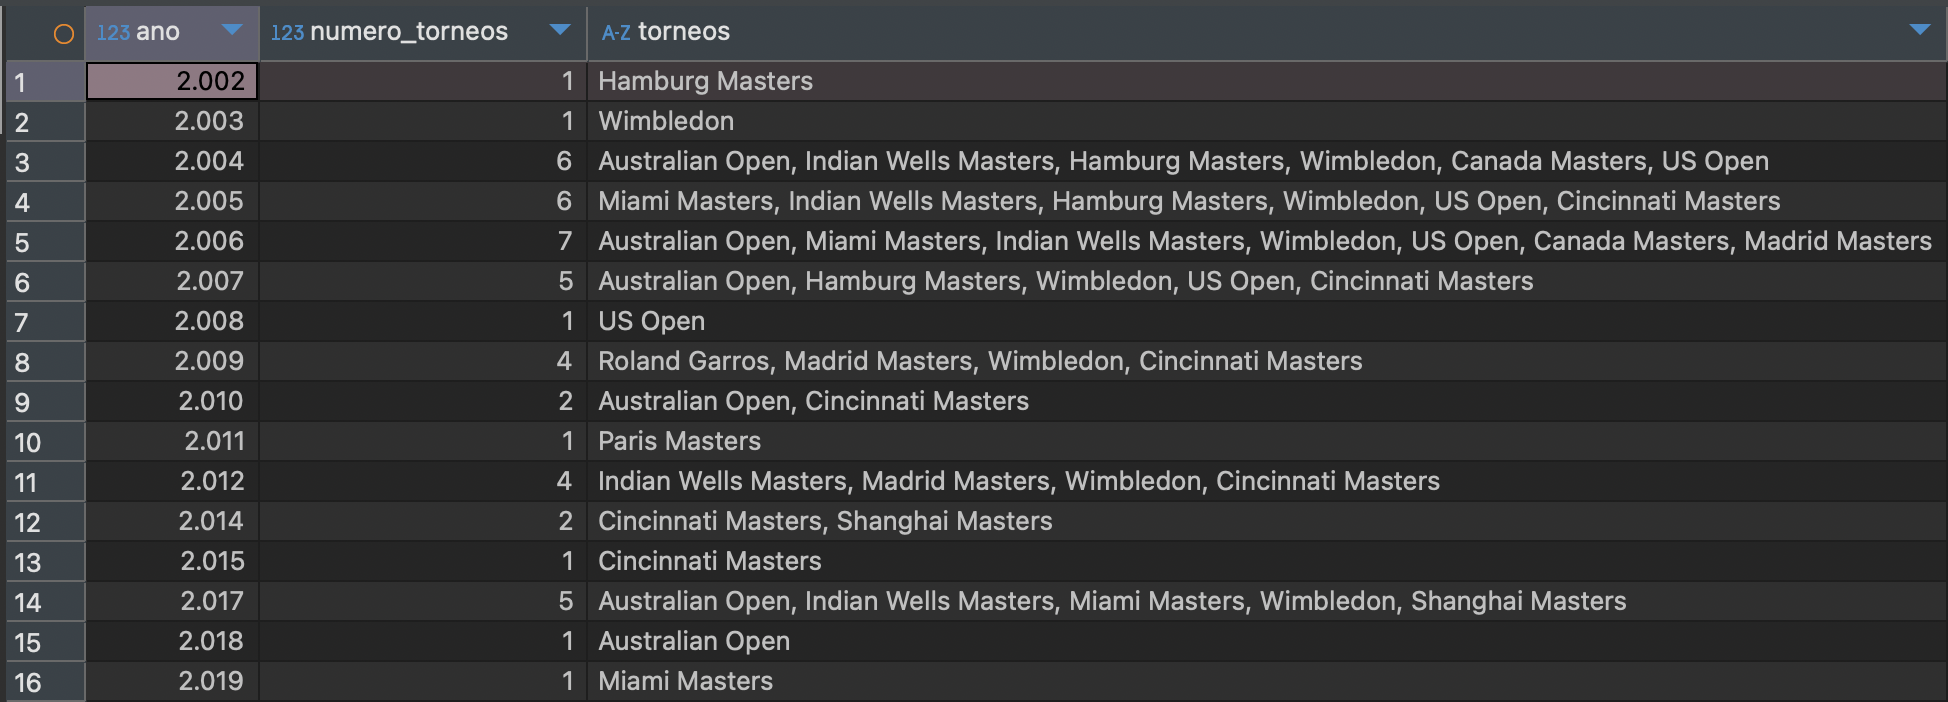
\includegraphics[width=0.8\textwidth]{fotos/q2_rel.png}
\caption{Modelo relacional Postgresql, consulta 2.}
\label{fig:q2_rel}
\end{figure}


\subsubsection{Muestra los partidos de semifinales (ronda='SF') y final (ronda = 'F') del torneo de "Roland Garros" del 2018. Para cada partido muestra la ronda, el tipo de desenlace, el nombre y apellidos del ganador y el nombre y apellidos del perdedor y el resultado con el número de juegos del ganador y del perdedor en cada set, y opcionalmente en paréntesis el número de juegos del perdedor en el tie break}

Para esta consulta necesitamos información de los partidos, los jugadores, los torneos y los sets de los partidos; como debemos distinguir entre el ganador y el perdedor, sin ningún tipo de ambigüedad, en el \texttt{from} usamos dos instancias de la tabla \texttt{jugador}, cada una con un alias distinto, por lo que estaremos haciendo el producto cartesiano de la tabla \texttt{jugador} consigo misma, así como con las tablas \texttt{partido}, \texttt{torneo} y \texttt{sets\_partido} (especificando un alias para cada una de ellas). A continuación, especificamos las condiciones de \textit{join} en el \texttt{where}, así como otras condiciones de selección:
\begin{itemize}
\item Condiciones de \textit{join} que, en global, nos permitirán seleccionar las tuplas de partidos específicos de un torneo específico en una fecha específica:
\begin{itemize}
\item El predicado \texttt{jg.id = p.ganador} sirve para unir la tabla \texttt{jugador} con la tabla \texttt{partido} mediante el atributo \texttt{id} de la tabla \texttt{jugador} y el atributo \texttt{ganador} de la tabla \texttt{partido}, haciendo una selección únicamente de las tuplas que cumplan esta condición. Esto nos permite, para cada jugador, seleccionar solo los partidos en los que ha ganado.
\item Del mismo modo, usamos el predicado \texttt{jp.id = p.perdedor} para eleccionar solo los partidos en los que ha perdido un determinado jugador. 
\item El predicado \texttt{p.fecha = sp.fecha} sirve para unir la tabla \texttt{partido} con la tabla \texttt{sets\_partido} mediante el atributo \texttt{fecha} de la tabla \texttt{partido} y el atributo \texttt{fecha} de la tabla \texttt{sets\_partido}, haciendo una selección únicamente de las tuplas que cumplan esta condición. Esto nos permite seleccionar solo los sets de los partidos que se han jugado en una fecha concreta.
\item Como la fecha anterior no es unívoca para cada partido, necesitamos una condición adicional para obtener los sets de un partido determinado. Para ello, usamos el predicado \texttt{p.num\_partido = sp.num\_partido}, que une la tabla \texttt{partido} con la tabla \texttt{sets\_partido} mediante el atributo \texttt{num\_partido} de la tabla \texttt{partido} y el atributo \texttt{num\_partido} de la tabla \texttt{sets\_partido}, haciendo una selección únicamente de las tuplas que cumplan esta condición.
\item El predicado \texttt{t.id = p.torneo} sirve para unir la tabla \texttt{torneo} con la tabla \texttt{partido} mediante el atributo \texttt{id} de la tabla \texttt{torneo} y el atributo \texttt{torneo} de la tabla \texttt{partido}, haciendo una selección únicamente de las tuplas que cumplan esta condición. Esto nos permite seleccionar solo los partidos que se han jugado en un torneo concreto.
\end{itemize}
\item Concretamente, estamos interesados en las semifinales (ronda='SF') y la final (ronda='F) del torneo de ``Roland Garros'' del 2018. Por tanto, las condiciones de selección son:
\begin{itemize}
\item El predicado \texttt{p.ronda in ('SF', 'F')} selecciona solo los partidos que han sido semifinales o finales.
\item El predicado \texttt{t.nombre = 'Roland Garros'} selecciona solo los partidos que se han jugado en el torneo ``Roland Garros''.
\item El predicado \texttt{extract(year from p.fecha) = '2018'} selecciona solo los partidos que se han jugado en el año 2018.
\end{itemize}
\end{itemize}

Ahora, para cada combinación de \texttt{p.ronda}, \texttt{p.desenlace}, \texttt{jg.nombre}, \texttt{jg.apellido}, \texttt{jp.nombre} y \texttt{jp.apellido}, tendremos una fila para cada set, donde solo variará la información de los juegos ganados y perdidos. Por tanto, agrupamos por los atributos mencionados anteriormente y, en la proyección, concatenamos los resultados de los juegos ganados y perdidos en cada set, así como el resultado final del partido, para lo que usamos la función \texttt{string\_agg()}. Como también debemos especificar la puntuación del \textit{tiebreak} (en caso de haberla), usamos un \texttt{case} para comprobar si el atributo \texttt{puntos\_tiebreak\_perdedor} es \texttt{null} o no: en caso que sea nulo, concatenamos una cadena vacia, en caso de no ser nulo, concatenamos la puntuación del \textit{tiebreak}, puesta entre paréntesis. Si bien esta es una parte de la proyección, el resto incluye simplemente la ronda, el desenlace, la fecha y los nombres y apellidos de los jugadores concatenados (un atributo para el ganador y otro para el perdedor). El código de la consulta se muestra a continuación, y el resultado se pueden ver en la figura \ref{fig:q3_rel}.

\begin{minted}[frame=single, fontsize=\footnotesize]{sql}
select p.ronda, p.desenlace, jg.nombre || ' ' || jg.apellido AS ganador, 
	jp.nombre || ' ' || jp.apellido AS perdedor, 
	STRING_AGG(sp.juegos_ganador || '-' || sp.juegos_perdedor ||
		case
		  when sp.puntos_tiebreak_perdedor is not null then 
		  	'(' || sp.puntos_tiebreak_perdedor || ')'
		  else 
		  	'' 
		end, ', ' order by sp.num_set) as resultado
from partido p, jugador jg, jugador jp, sets_partido sp, torneo t
where jg.id = p.ganador
  and jp.id = p.perdedor
  and p.fecha = sp.fecha
  and p.num_partido = sp.num_partido
  and t.id = p.torneo
  and p.ronda in ('SF', 'F')
  and t.nombre = 'Roland Garros'
  and extract(year from p.fecha) = '2018'
group by p.ronda, p.desenlace, jg.nombre, jg.apellido, jp.nombre, jp.apellido
\end{minted}

\begin{figure}[H]
\centering
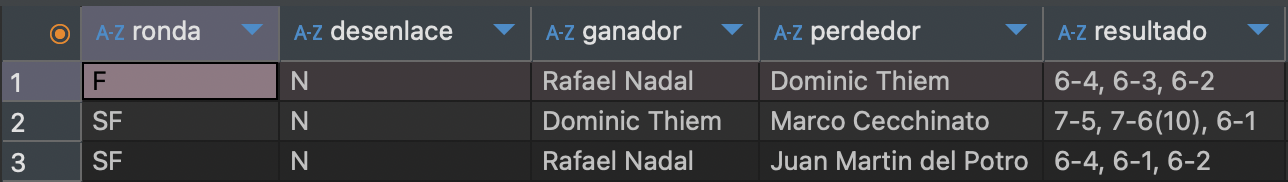
\includegraphics[width=0.7\textwidth]{fotos/q3_rel.png}
\caption{Modelo relacional Postgresql, consulta 3.}
\label{fig:q3_rel}
\end{figure}

\subsubsection{Muestra la lista de jugadores españoles (ES) que ganaron algún torneo de nivel Gran Slam (G). Para cada jugador muestra los siguientes datos resumen de todos sus partidos: número de partidos jugados, porcentaje de victorias, porcentaje de aces, porcentaje de dobles faltas, porcentaje de servicios ganados, porcentaje de restos ganados, porcentaje de break points salvados (de los sufridos en contra), porcentaje de break points ganados (de los provocados a favor)}

Esta consulta la dividiremos en dos partes: primero, buscaremos los jugadores españoles que ganaron algún torneo de nivel Grand Slam (G), y, a continuación, calcularemos los datos resumen que se piden de todos sus partidos. Para la primera parte, necesitamos información de los jugadores, los partidos y las ediciones de los torneos; comenzamos en el \texttt{from} con el producto cartesiano de las tablas \texttt{jugador}, \texttt{partido} y \texttt{edicion\_torneo} (especificando un alias para cada una de ellas). A continuación, especificamos las condiciones de \textit{join} en el \texttt{where}, así como otras condiciones de selección:
\begin{itemize}
\item Condiciones de \textit{join} que, en global, nos permitirán seleccionar las tuplas de un torneo específico:
\begin{itemize}
\item El predicado \texttt{j.id = p.ganador} sirve para unir la tabla \texttt{jugador} con la tabla \texttt{partido} mediante el atributo \texttt{id} de la tabla \texttt{jugador} y el atributo \texttt{ganador} de la tabla \texttt{partido}, haciendo una selección únicamente de las tuplas que cumplan esta condición. Esto nos permite, para cada jugador, seleccionar solo los partidos en los que ha ganado. 
\item El predicado \texttt{p.torneo = et.torneo} sirve para unir la tabla \texttt{partido} con la tabla \texttt{edicion\_torneo} mediante el atributo \texttt{torneo} de la tabla \texttt{partido} y el atributo \texttt{torneo} de la tabla \texttt{edicion\_torneo}, haciendo una selección únicamente de las tuplas que cumplan esta condición. Esto nos permite seleccionar solo los partidos que se han jugado en una edición concreta de un torneo.
\item El predicado \texttt{p.fecha = et.fecha} sirve para unir la tabla \texttt{partido} con la tabla \texttt{edicion\_torneo} mediante el atributo \texttt{fecha} de la tabla \texttt{partido} y el atributo \texttt{fecha} de la tabla \texttt{edicion\_torneo}, haciendo una selección únicamente de las tuplas que cumplan esta condición. Esto nos permite seleccionar solo los partidos que se han jugado en una fecha concreta.
\end{itemize}
\item Como de todo lo anterior solo nos interesan los partidos finales (F) de torneos de nivel Grand Slam (G) y ganados por jugadores españoles (ES), las condiciones de selección son:
\begin{itemize}
\item El predicado \texttt{p.ronda = `F'} selecciona solo los partidos que han sido finales.
\item El predicado \texttt{et.nivel = `G'} selecciona solo los torneos de nivel Grand Slam (G).
\item El predicado \texttt{j.pais = `ES'} selecciona solo los jugadores españoles.
\end{itemize}
\end{itemize}

Con todo esto, obtenemos una tabla con los jugadores españoles que han ganado algún torneo de nivel Grand Slam (G), pero hay repeticion ya que estamos considerando cada edición de cada Grand Slam. Para quedarnos solo con el subconjunto que nos interesa (sin repetición), usamos un \texttt{distinct} en la proyección. Concretamente, obtenemos la proyección del \texttt{id} y el nombre completo del jugador, que concatenamos con el operador \texttt{||}, y aplicamos el \texttt{distinct} sobre la proyección. Esta tabla resultado la guardamos como \texttt{jugadores\_espanoles\_ganadores}, y la usaremos en la segunda parte de la consulta. \\

Para obtener las estadísticas resumen de cada jugador español ganador de un Grand Slam, necesitamos solo información sobre quiénes son esos jugadores y sobre los partidos que han jugado. Por tanto, en el \texttt{from} usamos la tabla \texttt{jugadores\_espanoles\_ganadores} que acabamos de crear, y la tabla \texttt{partido} (especificando un alias para cada una de ellas). A continuación, especificamos las condiciones de \textit{join} en el \texttt{where}, así como otras condiciones de selección:
\begin{itemize}
\item Condiciones de \textit{join} que, en global, nos permitirán seleccionar las tuplas de partidos de un jugador específico:
\begin{itemize}
\item El predicado \texttt{jeg.id\_jugador = p.ganador or jeg.id\_jugador = p.perdedor} nos permite seleccionar los partidos, tanto ganados como perdidos, en los que ha participado un jugador específico de la tabla \texttt{jugadores\_espanoles\_ganadores}.
\end{itemize}
\end{itemize}

Con esto, obtenemos una fila por cada partido de cada jugador, por lo que agrupamos por el jugador con \texttt{group by} antes de agregar valores. En la proyección, obtenemos varios atributos, que redondearemos a un decimal usando \texttt{round(\dots, 1)}. En general, excepto para los partidos y el porcentaje de victorias, todas las estadísticas se calculan de la misma forma cosniderando atributos distintos; por ello, daremos una explicación detallada de una de ellas, y el resto simplemente mencionaremos qué atributos hemos usado y si se siguió un proceso distinto.
\begin{itemize}
\item El nombre completo del jugador, que concatenamos previamente con el operador \texttt{||}.
\item El número de partidos jugados como el conteo de los partidos en los que ha participado \\ (\texttt{count(p.num\_partido)}).
\item El porcentaje de victorias, que calculamos como el número de partidos ganados entre el número total de partidos jugados, multiplicado por 100. Para obtener el número de partidos ganados, usamos un \texttt{case} que comprueba si el jugador es el ganador del partido o no. Esto genera una lista que contiene 1 si el jugador es el ganador y 0 si no lo es, y con \texttt{sum()} sumamos los valores de esta lista para obtener el número de partidos ganados. 
\item El porcentaje de aces, que calculamos como el número de aces del jugador entre el número total de puntos servidos, multiplicado por 100. Para obtener el número de aces, simplemente sumamos (\texttt{sum()}) los valores la columna \texttt{num\_aces\_ganador} o \texttt{num\_aces\_perdedor} para el jugador específico. El número de puntos servidos lo obtenemos de forma análoga usando la columna \texttt{num\_ptos\_servidos\_ganador} o \texttt{num\_ptos\_servidos\_perdedor} según corresponda. Para ver si corresponde usar las estadísticas del ganador o del perdedor, se considerará un \texttt{case} que distinga si nuestro jugador está en la posición de ganador o perdedor, y se usarán las estadísticas correspondientes. Además, se implementará la función \texttt{nullif()} para gestionar las divisiones por 0. 
\item El porcentaje de dobles faltas, que calculamos de forma análoga al porcentaje de aces, pero usando las columnas \texttt{num\_dob\_faltas\_ganador} y \texttt{num\_dob\_faltas\_perdedor} en lugar de las columnas de aces. 
\item El porcentaje de servicios ganados, que calculamos de forma análoga al porcentaje de aces, pero usando una suma de las columnas \texttt{num\_primeros\_servicios\_ganados\_ganador} y \texttt{num\_segundos\_servicios\_gan-}\\\texttt{ados\_ganador}, o de \texttt{num\_primeros\_servicios\_ganados\_perdedor} y \texttt{num\_segundos\_servicios\_ganados}\\\texttt{\_perdedor} en lugar de las columnas de aces.
\item El porcentaje de restos ganados, que calculamos de forma análoga al porcentaje de aces. Sin embargo, está vez usaremos las estadísticas de rival para obtener la del jugador que nos interesa: si nuestro jugador ganó, nos fijaremos en \texttt{num\_ptos\_servidos\_perdedor} y \texttt{num\_restos\_ganados\_perdedor}, y si perdió, en \texttt{num\_ptos\_servidos\_perdedor}, \texttt{num\_primeros\_servicios\_ganados\_perdedor} y \texttt{p.num\_segundos\_servi-} \\ \texttt{cios\_ganados\_perdedor}, y si perdió, en los mismos atributos pero del ganador. El porcentaje de restos ganados por nuestro jugador será entonces el cociente entre el número de saques que su rival no consiguió ganar el servicio, que lo obtenemos como la resta entre los puntos servidos y los primeros y segundos servicios ganados, y el número total de puntos servidos por el rival, multiplicado por 100.
\item El porcentaje de \textit{breaks} salvados, que calculamos de forma análoga al porcentaje de aces pero usando las columnas \texttt{num\_break\_salvados\_ganador} o \texttt{num\_break\_salvados\_perdedor} en lugar de las columnas de aces, y \texttt{num\_break\_afrontados\_ganador} o \texttt{num\_break\_afrontados\_perdedor} en lugar de las columnas de puntos servidos.
\item El porcentaje de \textit{breaks} ganados, que calculamos de forma análoga al porcentaje de aces pero usando las estadísticas del rival. Lo obtenemos como el cociente entre la el número de \textit{breaks} que perdió el rival (calculado como la diferencia entre afrontados y ganados) y el número total de \textit{breaks} que afrontó el rival, multiplicado por 100.
\end{itemize}

\noindent A continuación se muestra la consulta completa y el resultado se puede ver en la figura \ref{fig:q4_rel}.

\begin{minted}[frame=single, fontsize=\footnotesize]{sql}
with jugadores_espanoles_ganadores as (
    select distinct j.id as id_jugador, j.nombre || ' ' || j.apellido as jugador
    from partido p, jugador j, edicion_torneo et 
    where p.ganador = j.id 
        and p.torneo = et.torneo 
        and p.fecha = et.fecha
        and j.pais = 'ES'
        and p.ronda = 'F'
        and et.nivel = 'G'
)

select jeg.jugador, count(p.num_partido) as partidos,
    round(100.0 * sum(case when jeg.id_jugador = p.ganador then 1 else 0 end) / 
		count(p.num_partido), 1) as pcje_victorias, 
    round(100.0 * sum(case when jeg.id_jugador = p.ganador then 
		p.num_aces_ganador else p.num_aces_perdedor end) / 
        nullif(sum(case when jeg.id_jugador = p.ganador then p.num_ptos_servidos_ganador 
		else p.num_ptos_servidos_perdedor end), 0), 1) as pcje_aces, 
    round(100.0 * sum(case when jeg.id_jugador = p.ganador then p.num_dob_faltas_ganador 
		else p.num_dob_faltas_perdedor  end) / 
        nullif(sum(case when jeg.id_jugador = p.ganador then p.num_ptos_servidos_ganador 
		else p.num_ptos_servidos_perdedor end), 0), 1) as pcje_dobles_faltas, 
    round(100.0 * sum(case when jeg.id_jugador = p.ganador then 
		p.num_primeros_servicios_ganados_ganador + p.num_segundos_servicios_ganados_ganador 
        else p.num_primeros_servicios_ganados_perdedor + p.num_segundos_servicios_ganados_perdedor end) / 
        nullif(sum(case when jeg.id_jugador = p.ganador then p.num_ptos_servidos_ganador 
		else p.num_ptos_servidos_perdedor end), 0), 1) as pcje_servicios_ganados, 
    round(100.0 * sum(case when jeg.id_jugador = p.ganador then 
		p.num_ptos_servidos_perdedor - p.num_primeros_servicios_ganados_perdedor - 
		p.num_segundos_servicios_ganados_perdedor 
        else p.num_ptos_servidos_ganador - p.num_primeros_servicios_ganados_ganador - 
		p.num_segundos_servicios_ganados_ganador end) / 
        nullif(sum(case when jeg.id_jugador = p.ganador then p.num_ptos_servidos_perdedor 
		else p.num_ptos_servidos_ganador end), 0), 1) as pcje_restos_ganados,
    round(100.0 * sum(case when jeg.id_jugador = p.ganador then p.num_break_salvados_ganador 
		else p.num_break_salvados_perdedor end) / 
        nullif(sum(case when jeg.id_jugador = p.ganador then p.num_break_afrontados_ganador 
		else p.num_break_afrontados_perdedor end), 0), 1) as pcje_breaks_salvados, 
    round(100.0 * sum(case when jeg.id_jugador = p.ganador then 
		p.num_break_afrontados_perdedor - p.num_break_salvados_perdedor 
        else p.num_break_afrontados_ganador - p.num_break_salvados_ganador end) / 
        nullif(sum(case when jeg.id_jugador = p.ganador then p.num_break_afrontados_perdedor 
		else p.num_break_afrontados_ganador end), 0), 1) as pcje_breaks_ganados
from jugadores_espanoles_ganadores jeg, partido p
where jeg.id_jugador = p.ganador 
	or jeg.id_jugador = p.perdedor
group by jeg.jugador
\end{minted}

\begin{figure}[H]
\centering
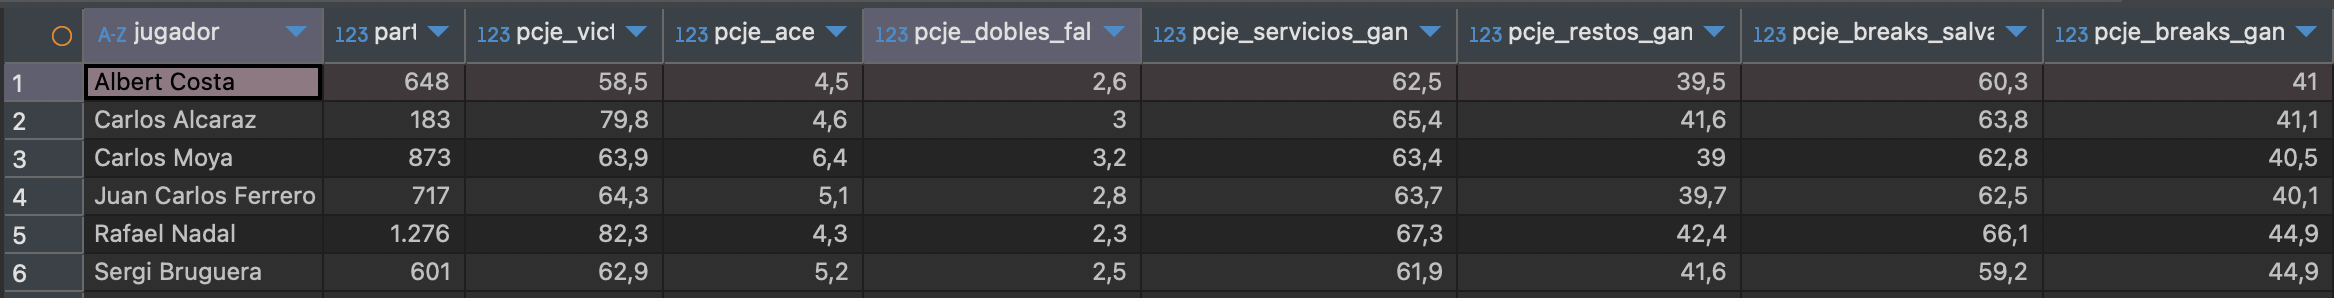
\includegraphics[width=\textwidth]{fotos/q4_rel.png}
\caption{Modelo relacional Postgresql, consulta 4.}
\label{fig:q4_rel}
\end{figure}

\subsubsection{Lista los jugadores que fueron derrotados (en algún partido del 2018) por el rival de Rafael Nadal de la primera ronda (R128) de Roland Garros de 2018}

Esta consulta la dividiremos de nuevo en dos partes. Primero, buscaremos el rival de Rafael Nadal en la primera ronda de Roland Garros de 2018, y, a continuación, buscaremos los jugadores que fueron derrotados por ese rival en algún partido de 2018. Para la primera parte, necesitamos información de los partidos, los jugadores, los torneos y sus ediciones; comenzamos en el \texttt{from} con el producto cartesiano de las tablas \texttt{jugador}, \texttt{partido}, \texttt{torneo} y \texttt{edicion\_torneo} (especificando un alias para cada una de ellas) Aquí, de nuevo, usamos la tabla \texttt{jugador} dos veces, una para identificar a un jugador (que será Rafael Nadal) y otra para identificar al rival sin ambigüedad. A continuación, especificamos las condiciones de \textit{join} en el \texttt{where}, así como otras condiciones de selección:
\begin{itemize}
\item Condiciones de \textit{join} que, en global, nos permitirán seleccionar las tuplas de partidos específicos:
\begin{itemize}
\item El predicado \texttt{jg.id = p.ganador} sirve para unir la tabla \texttt{jugador} con la tabla \texttt{partido} mediante el atributo \texttt{id} de la tabla \texttt{jugador} y el atributo \texttt{ganador} de la tabla \texttt{partido}, haciendo una selección únicamente de las tuplas que cumplan esta condición. Esto nos permite seleccionar solo los partidos en los que ganó un jugador concreto.
\item El predicado \texttt{jp.id = p.perdedor} sirve para unir la tabla \texttt{jugador} con la tabla \texttt{partido} mediante el atributo \texttt{id} de la tabla \texttt{jugador} y el atributo \texttt{perdedor} de la tabla \texttt{partido}, haciendo una selección únicamente de las tuplas que cumplan esta condición. Esto nos permite seleccionar solo los partidos en los que un jugador concreto es el perdedor del partido.
\item El predicado \texttt{p.torneo = et.torneo} sirve para unir la tabla \texttt{partido} con la tabla \texttt{edicion\_torneo} mediante el atributo \texttt{torneo} de la tabla \texttt{partido} y el atributo \texttt{torneo} de la tabla \texttt{edicion\_torneo}, haciendo una selección únicamente de las tuplas que cumplan esta condición. Esto nos permite seleccionar solo los partidos que se han jugado en una edición concreta de un torneo.
\item El predicado \texttt{p.fecha = et.fecha} sirve para unir la tabla \texttt{partido} con la tabla \texttt{edicion\_torneo} mediante el atributo \texttt{fecha} de la tabla \texttt{partido} y el atributo \texttt{fecha} de la tabla \texttt{edicion\_torneo}, haciendo una selección únicamente de las tuplas que cumplan esta condición. Esto nos permite seleccionar solo los partidos que se han jugado en una fecha concreta.
\item El predicado \texttt{t.id = et.torneo} sirve para unir la tabla \texttt{torneo} con la tabla \texttt{edicion\_torneo} mediante el atributo \texttt{id} de la tabla \texttt{torneo} y el atributo \texttt{torneo} de la tabla \texttt{edicion\_torneo}, haciendo una selección únicamente de las tuplas que cumplan esta condición. Esto nos permite seleccionar solo los torneos que se han jugado en una edición concreta.
\end{itemize}
\item Ahora, queremos especificar que ese rival sea Rafael Nadal (no sabemos si ganó o perdió), que el torneo sea Roland Garros de 2018 y que la ronda sea la primera ronda (R128). Por tanto, las condiciones de selección son:
\item El predicado \texttt{p.ronda = `R128'} selecciona solo los partidos que han sido de la primera ronda.
\item El predicado \texttt{t.nombre = `Roland Garros'} selecciona solo los partidos que se han jugado en el torneo ``Roland Garros''.
\item El predicado \texttt{extract(year from p.fecha) = `2018'} selecciona solo los partidos que se han jugado en el año 2018.
\item El predicado \texttt{jg.nombre = `Rafael' and jg.apellido = `Nadal' or jp.nombre = `Rafael' and}\\ \texttt{jp.apellido = `Nadal'} selecciona solo los partidos en los que ha participado Rafael Nadal, ya sea como ganador o como perdedor.
\end{itemize}

El resultado es entonces una única tupla, con ese partido de primera ronda de Roland Garros 2018. Como queremos la información del rival, obtenemos como proyección su \texttt{id} y su nombre completo, que concatenamos con el operador \texttt{||}. Al no conocer de antemano si Rafael Nadal ganó o perdió, no podemos saber si el rival fue el ganador o el perdedor, por lo que debemos usar un \texttt{case} para seleccionar al ganador si Nadal fue el perdedor y viceversa. Guardamos esta información en una tabla llamada \texttt{rival\_nadal}, que usaremos en la segunda parte de la consulta. \\

La segunda parte de la consulta es más simple: queremos ver que jugadores perdieron contra este rival en el año 2018. Por tanto, necesitamos información de los jugadores, los partidos y la tabla \texttt{rival\_nadal}; comenzamos en el \texttt{from} con el producto cartesiano de las tablas \texttt{jugador}, \texttt{partido} y \texttt{rival\_nadal} (especificando un alias para cada una de ellas). A continuación, especificamos las condiciones de \textit{join} en el \texttt{where}, así como otras condiciones de selección:
\begin{itemize}
\item Condiciones de \textit{join} que, en global, nos permitirán seleccionar las tuplas de partidos específicos:
\begin{itemize}
\item El predicado \texttt{rn.id\_jugador = p.ganador} nos permite seleccionar solo los partidos en los que el rival de Rafael Nadal anterior fue el ganador.
\item El predicado \texttt{p.perdedor = j.id} nos permite seleccionar solo los partidos en los que el perdedor fue un jugador específico.
\end{itemize}
\item Ya con esto tenemos tuplas de los partidos ganados por el rival, pero falta especificar el año con la siguiente condición de selección: 
\begin{itemize}
\item El predicado \texttt{extract(year from p.fecha) = '2018'} selecciona solo los partidos que se han jugado en el año 2018.
\end{itemize}
\end{itemize}

Esto nos devuelve las tuplas de partidos de 2018 con el rival de Nadal como ganador, y al no haber repetición, no es necesario usar un \texttt{distinct}. En la proyección, obtenemos el nombre completo del jugador perdedor y su país, que mostraremos como el código iso 2 correspondiente. El código de la consulta se muestra a continuación, y el resultado se puede ver en la figura \ref{fig:q5_rel}.

\begin{minted}[frame=single, fontsize=\footnotesize]{sql}
with rival_nadal as (
	select case when jg.nombre = 'Rafael' then jp.id else jg.id end as id_jugador, 
		case when jg.nombre = 'Rafael' then jp.nombre || ' ' || jp.apellido 
		else jg.nombre || ' ' || jg.apellido end as jugador
	from partido p, jugador jg, jugador jp, edicion_torneo et, torneo t
	where p.ganador = jg.id 
		and p.perdedor = jp.id
		and p.torneo = et.torneo 
		and p.fecha = et.fecha
		and et.torneo = t.id 
		and t.nombre = 'Roland Garros'
		and p.ronda = 'R128'
		and extract(year from p.fecha) = '2018'
		and (jg.nombre = 'Rafael' and jg.apellido = 'Nadal' 
		or jp.nombre = 'Rafael' and jp.apellido = 'Nadal') 
)

select j.nombre || ' ' || j.apellido as jugador, j.pais as pais
from rival_nadal rn, partido p, jugador j
where rn.id_jugador = p.ganador 
	and p.perdedor = j.id
	and extract(year from p.fecha) = '2018'
\end{minted}

\begin{figure}[H]
\centering
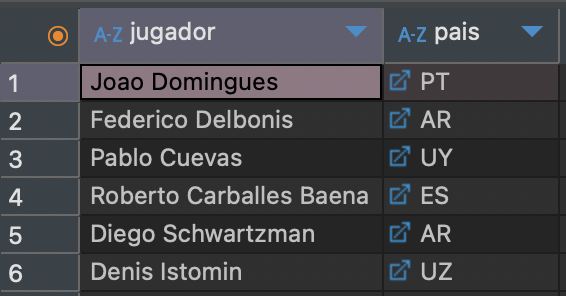
\includegraphics[width=0.35\textwidth]{fotos/q5_rel.png}
\caption{Modelo relacional Postgresql, consulta 5.}
\label{fig:q5_rel}
\end{figure}




\section{Datos agregados en SQL (PostgreSQL)}

A continuación, queremos crear una tabla que contenga todos los datos de los partidos (países, torneos, ediciones, partidos, sets y jugadores), pero con datos agregados. Concretamente, debemos definir estructuras que permitan resolver de forma eficiente las consultas Q1 y Q3 de la sección anterior. Para mantener orden en nuestra base de datos, crearemos un nuevo esquema \texttt{agregados} para alojar esta nueva tabla. \\

El sistema de tipos de PostgreSQL tiene constructores de tipo \texttt{ROW}, para tipos compuestos, y \texttt{ARRAY} para colecciones (en nuestro caso usaremos solo arrays unidimensionales). Para definir una tabla con tipos compuestos que resuelva eficientemente las consultas deseadas, el esquema debe ir orientado a los partidos en lugar de a los jugadores. Buscaremos definir entonces un esquema donde cada fila de la tabla represente un partido. Para ello, definimos los siguientes tipos:

\subsection{Tipos compuestos}

\begin{itemize}
\item \texttt{pais\_info}: contiene información sobre un país, con los campos originales de dicha tabla: \texttt{codigo\_iso2}, \texttt{codigo\_iso3}, \texttt{codigo\_ioc} y \texttt{nombre}.
\begin{minted}[frame=single, fontsize=\footnotesize]{sql}
create type pais_info as (
	codigo_iso2 char(2),
	codigo_iso3 char(3),
	codigo_ioc char(3),
	nombre varchar(100)
)
\end{minted}
\item \texttt{torneo\_info}: contiene información sobre un torneo, con los campos originales de dicha tabla: \texttt{id}, \texttt{nombre} y \texttt{pais}. El campo \texttt{pais} será de tipo \texttt{pais\_info}.
\begin{minted}[frame=single, fontsize=\footnotesize]{sql}
create type torneo_info as (
	id integer,
	nombre varchar(100),
	pais pais_info
)
\end{minted}
\item \texttt{edicion\_torneo\_info}: contiene información sobre una edición de un torneo, con los campos originales de dicha tabla: \texttt{torneo}, \texttt{fecha}, \texttt{superficie}, \texttt{tamano} y \texttt{nivel}. El campo \texttt{torneo} será de tipo \texttt{torneo\_info}.
\begin{minted}[frame=single, fontsize=\footnotesize]{sql}
create type edicion_torneo_info as (
	torneo torneo_info,
	fecha date,
	superficie varchar(20),
	tamano integer,
	nivel char(1)
)
\end{minted}
\item \texttt{set\_info}: contiene información sobre un set de un partido, con los campos originales de su tabla correspondiente: \texttt{torneo}, \texttt{fecha}, \texttt{num\_partido}, \texttt{num\_set}, \texttt{juegos\_ganador}, \texttt{juegos\_perdedor} y \texttt{puntos\_tiebreak}\\\texttt{\_perdedor}. El campo \texttt{torneo} será de tipo \texttt{torneo\_info}.
\begin{minted}[frame=single, fontsize=\footnotesize]{sql}
create type set_info as (
	torneo torneo_info,
	fecha date, 
	num_partido integer,
    num_set integer,
	juegos_ganador integer,
	juegos_perdedor integer,
	puntos_tiebreak_perdedor integer
)
\end{minted}
\item La tabla original de partidos tenía mucha información, ya que incluía estadísticas del ganador y del perdedor. Para simplificar, definimos un tipo \texttt{jugador\_stats} que contenga solo las estadísticas de un jugador en un partido, con las estadísticas que se daban en la tabla \texttt{partido}: \texttt{num\_aces}, \texttt{num\_dob\_faltas}, \texttt{num\_ptos\_servidos}, \texttt{num\_primeros\_servicios}, \texttt{num\_primeros\_servicios\_ganados}, \texttt{num\_segundos\_ser-}\\\texttt{vicios\_ganados}, \texttt{num\_juegos\_servidos}, \texttt{num\_break\_salvados} y \texttt{num\_break\_afrontados}.
\begin{minted}[frame=single, fontsize=\footnotesize]{sql}
create type jugador_stats as (
	num_aces integer,
	num_dob_faltas integer,
	num_ptos_servidos integer,
	num_primeros_servicios integer,
	num_primeros_servicios_ganados integer,
	num_segundos_servicios_ganados integer,
	num_juegos_servidos integer,
	num_break_salvados integer,
	num_break_afrontados integer
)
\end{minted}
\item \texttt{jugador\_info}: contiene información sobre un jugador, con los campos originales de dicha tabla: \texttt{id}, \texttt{nombre}, \texttt{apellido}, \texttt{diestro}, \texttt{fecha\_nacimiento}, \texttt{pais} y \texttt{altura}. El campo \texttt{pais} será de tipo \texttt{pais\_info}.
\begin{minted}[frame=single, fontsize=\footnotesize]{sql}
create type jugador_info as (
   id integer,
   nombre varchar(100),
   apellido varchar(100),
   diesto boolean,
   fecha_nacimiento date,
   pais pais_info,
   altura integer
)
\end{minted}
\item La tabla que unifique todo será \texttt{partidos} y, como comentamos, tendrá una fila por cada partido. Los campos serán los originales de la tabla \texttt{partido}, pero con los tipos compuestos que acabamos de definir: \texttt{torneo} será de tipo \texttt{torneo\_info}, \texttt{ganador} y \texttt{perdedor} serán de tipo \texttt{jugador\_info}, y \texttt{ganador\_stats} y \texttt{perdedor\_stats} serán de tipo \texttt{jugador\_stats} (almacenamos las estadísticas de una forma mucho más limpia). Además, el campo \texttt{info\_sets} será un array de elementos de tipo \texttt{set\_info} (al ser el array homogéneo y declarar que todos los elementos sean del mismo tipo, aunque sea un tipo compuesto, podemos definir el array).
\begin{minted}[frame=single, fontsize=\footnotesize]{sql}
create table partidos (
	torneo edicion_torneo_info,
	fecha date,
	num_partido integer,
	num_sets integer,
	info_sets set_info array, -- array de elementos de tipo set_info
	ronda varchar(5), 
	desenlace char(1), 
	ganador jugador_info,
	perdedor jugador_info,
	ganador_stats jugador_stats,
	perdedor_stats jugador_stats
)
\end{minted}
\end{itemize}

Una vez construida la tabla, queremos construir sus filas (insertar datos) a partir de las tablas del modelo relacional antes usado. Antes de introducir datos en un tipo compuesto, verificaremos que la clave primaria que tenía ese registro en la tabla relacional no sea nula y, en caso de serlo, insertaremos un null en lugar del registro. Para ello, usaremos un \texttt{case}. La función \texttt{cast()} nos permitirá agrupar valores individuales dentro de un tipo compuesto. Esto deberemos usarlo cada vez que queramos insertar un país, un torneo, la informacion de un set, las estadísticas de los jugadores o los propios jugadores. \\

Lo primero es seleccionar las tablas a usar en el \texttt{from}. Partimos del producto cartesiano entre \texttt{partido}, \texttt{edicion\_torneo}, \texttt{torneo}, \texttt{pais} (3 veces, una para el país del torneo, otra para el país del ganador y otra para el país del perdedor) y \texttt{jugador} (2 veces, una para el ganador y otra para el perdedor). En este caso, las condiciones de \textit{join}, así como el tipo, son muy importantes, ya que podemos perder información por el camino. 
\begin{itemize}
\item Usamos un \textit{inner join} para unir las tablas \texttt{partido} y \texttt{edicion\_torneo} mediante los campos \texttt{fecha} y \texttt{torneo}. Esto nos permite seleccionar solo los partidos que se han jugado en una edición concreta de un torneo.
\item Usamos un \textit{inner join} para unir las tablas \texttt{edicion\_torneo} y \texttt{torneo} mediante el campo \texttt{torneo}. Esto nos permite seleccionar ediciones de un torneo concreto.
\item Usamos un \textit{left join} para unir las tablas \texttt{torneo} y \texttt{pais} mediante el campo \texttt{pais}. Esto nos permite seleccionar torneos que se han jugado en un país concreto. Importante usar aquí un \textit{left join} para no perder información de los torneos que no tienen país registrado, como son \textit{ATP Cup}, \textit{Tour Finals} y \textit{Masters Cup} (\texttt{NULL}).
\item Usamos un \textit{left join} para unir las tablas \texttt{partido} y \texttt{jugador} mediante el campo \texttt{ganador}. Esto nos permite seleccionar los jugadores que han ganado un partido concreto. Importante usar aquí un \textit{left join} para no perder información de los partidos que no tienen ganador registrado (\texttt{NULL}).
\item Usamos un \textit{left join} para unir las tablas \texttt{jugador} y \texttt{pais} mediante el campo \texttt{pais} (para el ganador). Esto nos permite seleccionar jugadores que son de un país concreto. Aquí usamos un \textit{left join} para no perder información de los jugadores que no tienen país registrado (\texttt{NULL}) o cuyo pais no está en la tabla \texttt{pais}. Con unas consultas sencillas se puede comprobar que actualmente no existe este problema, pero haciendo un \textit{inner join} perdemos 2 registros del total, por lo que un \textit{left join} asegura que no perdamos información.
\item Usamos un \textit{left join} para unir las tablas \texttt{partido} y \texttt{jugador} mediante el campo \texttt{perdedor}. Esto nos permite seleccionar los jugadores que han perdido un partido concreto. Importante usar aquí un \textit{left join} para no perder información de los partidos que no tienen perdedor registrado (\texttt{NULL}). 
\item Usamos un \textit{left join} para unir las tablas \texttt{jugador} y \texttt{pais} mediante el campo \texttt{pais} (para el perdedor). Esto nos permite seleccionar jugadores que son de un país concreto. Aquí usamos un \textit{left join} por la misma razón que antes: aparentemente no hay inconsistencias, pero si cambiamos este por un \textit{inner join}, perdemos un total de 5 registros. 
\end{itemize}

Explicamos ahora brevemente el proceso de inserción de datos en la tabla \texttt{partidos}, una vez definido el producto del cual haremos una proyección:
\begin{itemize}
\item Comenzamos con el atributo \texttt{torneo}, de tipo \texttt{edicion\_torneo\_info}. Usamos un \texttt{case} para comprobar si el torneo existe en la tabla \texttt{torneo}. Si no existe, insertamos un \texttt{null}. si existe, insertamos valores en los atributos que marca este tipo compuesto: fecha, superficie, tamaño y nivel vendrán de la tabla \texttt{edicion\_torneo}, mientras que \texttt{torneo} debemos ``castearlo'' al tipo \texttt{torneo\_info}, introduciendo sus atributos. Los atributos de este tipo vienen todos de la tabla \texttt{torneo} excepto el país, que se debe ``castear'' al tipo \texttt{pais\_info} y tomará sus atributos de la tabla \texttt{pais}.
\item Los atributos \texttt{fecha}, \texttt{num\_partido}, \texttt{num\_sets}, \texttt{ronda} y \texttt{desenlace} se insertan directamente de la tabla \texttt{partido}.
\item El atributo \texttt{info\_sets} es un array de elementos de tipo \texttt{set\_info}. Para construirlo, usamos un \texttt{array} con una subconsulta que selecciona los sets de un partido concreto. Cada set se construye con un \texttt{cast} que agrupa los valores de la tabla \texttt{sets\_partido} en un tipo compuesto \texttt{set\_info}. \\

En dicha subconsulta, en la que solo usamos la tabla \texttt{sets\_partido}, fijamos condiciones de \textit{join} para unir esta tabla con la tabla \texttt{partido}, mediante los campos \texttt{torneo}, \texttt{fecha} y \texttt{num\_partido}. Así, obtenemos la información relativa a los sets de un partido concreto. Ordenamos en orden ascendente según el número del set y, finalmente, obtenemos la proyección de la información de los sets de ese partido.
\item Los atributos \texttt{ganador} y \texttt{perdedor} son de tipo \texttt{jugador\_info} y los obtenemos de forma completamente análoga. Usamos un \texttt{case} para comprobar si el ganador o el perdedor existen en la tabla \texttt{jugador}. Si no existen, insertamos un \texttt{null}. Si existen, insertamos valores en los atributos que marca este tipo compuesto: nombre, apellido, diestro, fecha de nacimiento y altura vendrán de la tabla \texttt{jugador}. El país se debe ``castear'' al tipo \texttt{pais\_info} y tomará sus atributos de la tabla \texttt{pais}.
\item Los atributos \texttt{ganador\_stats} y \texttt{perdedor\_stats} son de tipo \texttt{jugador\_stats} y los obtenemos de forma completamente análoga. Usamos un \texttt{case} para comprobar si el ganador o el perdedor existen en la tabla \texttt{jugador}. Si no existen, insertamos un \texttt{null}. Si existen, insertamos valores en los atributos que marca este tipo compuesto: número de aces, dobles faltas, puntos servidos, primeros servicios, primeros servicios ganados, segundos servicios ganados, juegos servidos, breaks salvados y breaks afrontados vendrán todos dados por la tabla \texttt{partido}, para el jugador que se esté usando.
\end{itemize}

\noindent A continuación, la consulta para insertar los datos en nuestra nueva tabla desde la base de datos relacional.


\begin{minted}[frame=single, fontsize=\footnotesize]{sql}
insert into partidos(
torneo, fecha, num_partido, num_sets, info_sets, ronda, desenlace, ganador, perdedor, 
ganador_stats, perdedor_stats)
select
   -- campo 'torneo' (tipo 'edicion_torneo_info')
   case
       when t.id is null then null
       else cast((cast((t.id, t.nombre, cast((pa.codigo_iso2, pa.codigo_iso3, pa.codigo_ioc, 
	   pa.nombre) as pais_info)) as torneo_info), 
       et.fecha, et.superficie, et.tamano, et.nivel) as edicion_torneo_info)
   end as torneo,
  
   p.fecha as fecha,
   p.num_partido as num_partido,
   p.num_sets as num_sets,
  
   -- campo 'info_set' (array de 'set_info')
   array(select cast((cast((t.id, t.nombre, cast((pa.codigo_iso2, pa.codigo_iso3, pa.codigo_ioc, 
   pa.nombre) as pais_info)) as torneo_info),
                      sp.fecha, sp.num_partido, sp.num_set, sp.juegos_ganador, sp.juegos_perdedor, 
					  sp.puntos_tiebreak_perdedor) as set_info)
         from public.sets_partido sp
         where sp.torneo = p.torneo
         	and sp.fecha = p.fecha
         	and sp.num_partido = p.num_partido
         order by sp.num_set) as info_sets,
  
   p.ronda as ronda,
   p.desenlace as desenlace,
  
   -- campo 'ganador' (tipo 'jugador_info')
   case
       when jg.id is null then null
       else cast((jg.id, jg.nombre, jg.apellido, jg.diestro, jg.fecha_nacimiento,
       		   cast((pg.codigo_iso2, pg.codigo_iso3, pg.codigo_ioc, pg.nombre) as pais_info),
       		   jg.altura) as jugador_info)
   end as ganador,
  
   -- campo 'perdedor' (tipo 'jugador_info')
   case
       when jp.id is null then null
       else cast((jp.id, jp.nombre, jp.apellido, jp.diestro, jp.fecha_nacimiento,
       		   cast((pp.codigo_iso2, pp.codigo_iso3, pp.codigo_ioc, pp.nombre) as pais_info),
       		   jp.altura) as jugador_info)
   end as perdedor,
  
   -- campo 'ganador_stats' (tipo 'jugador_stats')
   case
       when jg.id is null and jp.id is null then null
       else cast((p.num_aces_ganador, p.num_dob_faltas_ganador,
           	   p.num_ptos_servidos_ganador, p.num_primeros_servicios_ganador,
           	   p.num_primeros_servicios_ganados_ganador, p.num_segundos_servicios_ganados_ganador,
           	   p.num_juegos_servidos_ganador, p.num_break_salvados_ganador,
           	   p.num_break_afrontados_ganador) as jugador_stats)
   end as ganador_stats,
  
   -- campo 'perdedor_stats' (tipo 'jugador_stats')
   case
       when jg.id is null and jp.id is null then null
       else cast((p.num_aces_perdedor, p.num_dob_faltas_perdedor,
           	   p.num_ptos_servidos_perdedor, p.num_primeros_servicios_perdedor,
           	   p.num_primeros_servicios_ganados_perdedor, p.num_segundos_servicios_ganados_perdedor,
           	   p.num_juegos_servidos_perdedor, p.num_break_salvados_perdedor,
           	   p.num_break_afrontados_perdedor) as jugador_stats)
   end as perdedor_stats
from public.partido p join public.edicion_torneo et on et.fecha = p.fecha and et.torneo = p.torneo 
	join public.torneo t on t.id = et.torneo
	left join public.pais pa on t.pais = pa.codigo_iso2
	left join public.jugador jg on p.ganador = jg.id
	left join public.pais pg on jg.pais = pg.codigo_iso2
	left join public.jugador jp on p.perdedor = jp.id
	left join public.pais pp on jp.pais = pp.codigo_iso2
\end{minted}



\subsubsection{Muestra todos los ganadores del torneo ``Wimbledon'' (Nombre apellidos y año). Ordena el resultado por año.}

Para reescribir esta consulta, debemos tener en cuenta que ahora solo existe una tabla, por lo que no necesitamos hacer productos cartesianos ni \textit{joins}. Simplemente, especificamos condiciones sobre los campos y seleccionamos los campos que queremos mostrar. Para acceder a un campo dentro de un tipo compuesto que sea columna de la tabla, será necesario usar paréntesis; veámoslo en la siguiente consulta. \\

Partiendo de la tabla partidos, seleccionamos aquellos cuyo torneo sea ``Wimbledon'' y la ronda sea ``F'' (final). A la ronda se accede de forma fácil, al ser un atributo de la propia tabla partidos. Sin embargo, para acceder al nombre del torneo, debemos acceder a nombre, dentro de torneo (de tipo \texttt{torneo\_info}), dentro de torneo (de tipo \texttt{edicion\_torneo}). Para ello, debemos usar paréntesis para acceder al primer torneo: \texttt{(torneo).torneo.nombre}. Equivalentemente, podríamos haber usado \texttt{((torneo).torneo).nombre}, pero al acceder primero al tipo compuesto, el gestor ya tiene claro que esa columna se trata de un tipo compuesto y no requiere una segunda aclaración con el doble paréntesis. \\

Tras la selección, tenemos un conjunto de tuplas con los partidos finales de Wimbledon. Obtenemos como proyección el nombre y apellido del ganador (campos a los cuales debemos acceder mediante \texttt{(ganador)}, al ser un tipo compuesto), y el año de la edición del torneo, que lo obtenemos con un simple \texttt{extract}. Para terminar, ordenamos el resultado por año. La consulta se muestra a continuación y el resultado, que coincide con lo esperado, se puede ver en la figura \ref{fig:q1_com}.

\begin{minted}[frame=single, fontsize=\footnotesize]{sql}
select (ganador).nombre, (ganador).apellido, extract(year from fecha) as ano
from partidos
where (torneo).torneo.nombre = 'Wimbledon'
	and ronda = 'F'
order by ano
\end{minted}

\begin{figure}[H]
\centering
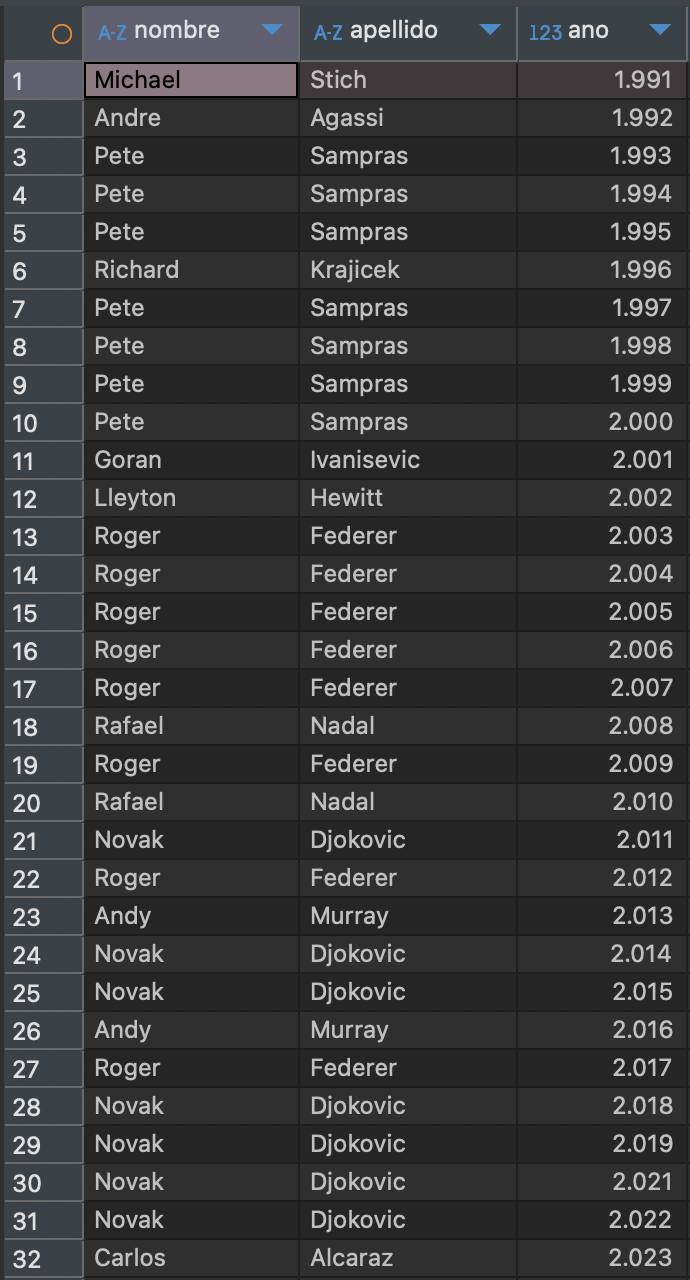
\includegraphics[height=0.4\textheight]{fotos/q1_com.png}
\caption{Datos agregados en SQL. Tipos compuestos, consulta 1.}
\label{fig:q1_com}
\end{figure}


\subsubsection{Muestra los años en los que Roger Federer ganó algún torneo de nivel Gran Slam (G) o Master 1000 (M). Para cada año, muestra el número de torneos y lista sus nombres (ordenados por la fecha de celebración). Ordena el resultado por el año}

Para reescribir esta consulta, usamos la única tabla de la que disponemos. Fijamos como condiciones de selección que el nombre del ganador sea Roger y el apellido Federer (campos a los que accedemos mediante \texttt{ganador}, que es un tipo compuesto), que el nivel del torneo sea G o M (accedemos a nivel mediante \texttt{(torneo).nivel}, ya que nivel es un campo del atributo \texttt{torneo}, de tipo \texttt{edicion\_torneo}) y que la ronda sea final (F). Esto nos devuelve una tupla para cada partido final de un Grand Slam o Master 1000 que Roger Federer ha ganado. Agrupamos esto por año, que lo obtenemos desde la fecha del torneo, a la cual accedemos a través del tipo \texttt{torneo} como \texttt{(torneo).fecha}, para obtener una única fila para cada año. Como proyección nos quedamos con el año del torneo (de los torneos concretamente), el número de torneos que hay en esa agrupación (los podemos contar por el número de \texttt{id} distintos que haya, accediendo a \texttt{(torneo).torneo.id}), y una concatenación del nombre de los torneos ganados ese año por Federer ordenada por fecha (el campo \texttt{nombre} lo encontramos, de nuevo, accediendo a \texttt{(torneo).torneo}). A continuación, mostramos la consulta y el resultado, que coincide con lo esperado, se puede ver en la figura \ref{fig:q2_com}.

\begin{minted}[frame=single, fontsize=\footnotesize]{sql}
select extract(year from (torneo).fecha) as ano, count(distinct (torneo).torneo.id) as numero_torneos, 
	string_agg((torneo).torneo.nombre, ', ' order by (torneo).fecha) as torneos
from partidos
where (torneo).nivel in ('G', 'M')
	and (ganador).nombre = 'Roger'
	and (ganador).apellido = 'Federer'
	and ronda = 'F'
group by ano
\end{minted}

\begin{figure}[H]
\centering
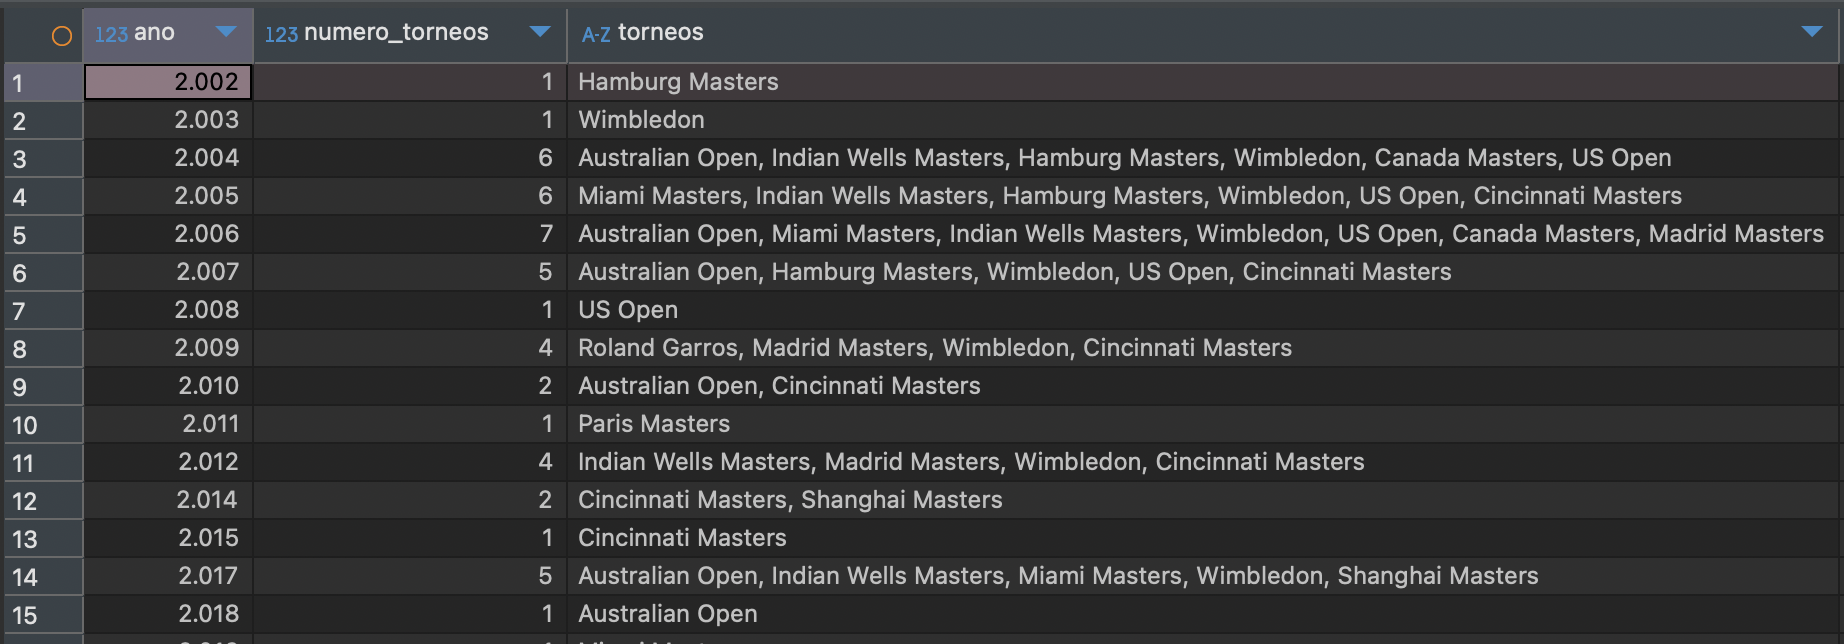
\includegraphics[width=0.8\textwidth]{fotos/q2_com.png}
\caption{Datos agregados en SQL. Tipos compuestos, consulta 2.}
\label{fig:q2_com}
\end{figure}





\subsubsection{Muestra los partidos de semifinales (ronda='SF') y final (ronda = 'F') del torneo de "Roland Garros" del 2018. Para cada partido muestra la ronda, el tipo de desenlace, el nombre y apellidos del ganador y el nombre y apellidos del perdedor y el resultado con el número de juegos del ganador y del perdedor en cada set, y opcionalmente en paréntesis el número de juegos del perdedor en el tie break}

En este caso, las condiciones de selección que deben ir en el \texttt{where} son la ronda (semifinal o final), el nombre del torneo (Roland Garros) y el año (2018). Para cada partido, queremos mostrar la ronda, el desenlace, el nombre y apellidos del ganador y del perdedor, y el resultado con el número de juegos del ganador y del perdedor en cada set. Para ello, debemos acceder a los campos de los tipos compuestos que hemos definido. Todo esto se obtiene de forma fácil y directa accediendo a las columnas necesarios, usando paréntesis en caso de que esa columna se un tipo compuesto, a excepción de la información de los sets. Veamos esto en concreto con un poco más de detalle. \\

Para obtener la información de los sets, debemos acceder a la columna \texttt{info\_sets}, que es un array con elementos de tipo compuesto. Para acceder a sus elementos, debemos hacer una subconsulta donde desagreguemos el array en el \texttt{from} con la función \texttt{unnest}. Tras desagregar el array, se trata como una consulta estándar y accedemos a los campos de los elementos del array como si fueran columnas de una tabla. En este caso, accedemos a los campos \texttt{juegos\_ganador}, \texttt{juegos\_perdedor} y \texttt{puntos\_tiebreak\_perdedor} de cada set. Para mostrar estos datos de forma más clara, concatenamos los resultados en un solo string con la función \texttt{string\_agg}, mostrando la puntuación del \textit{tiebreak} solo si existe. Además, esta concatenación se hace por orden ascendente según el número del set. Así, obtenemos una única tupla con los información de los sets de un partido. La consulta y el resultado, que coincide con lo esperado, se pueden ver en la figura \ref{fig:q3_com}.

\begin{minted}[frame=single, fontsize=\footnotesize]{sql}
select ronda, desenlace, 
	(ganador).nombre || ' ' || (ganador).apellido as ganador,
	(perdedor).nombre || ' ' || (perdedor).apellido as perdedor, 
	(select string_agg(iset.juegos_ganador || '-' || iset.juegos_perdedor ||
	case
		when iset.puntos_tiebreak_perdedor is not null then 
			'(' || iset.puntos_tiebreak_perdedor || ')'
		else ''
	end, ', ' order by iset.num_set) 
	from unnest(info_sets) as iset) as resultado
from partidos
where ronda in ('SF', 'F')
	and (torneo).torneo.nombre = 'Roland Garros'
	and extract(year from fecha) = '2018'
\end{minted}

\begin{figure}[H]
\centering
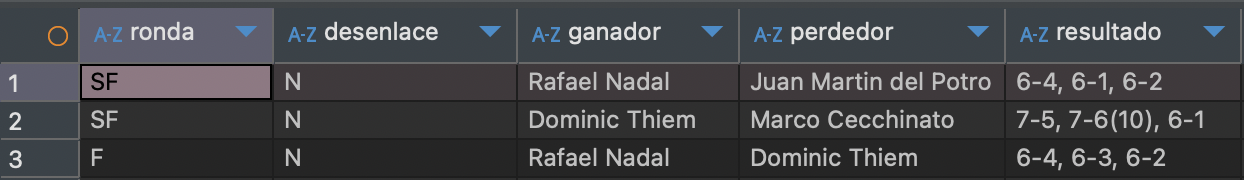
\includegraphics[width=0.7\textwidth]{fotos/q3_com.png}
\caption{Datos agregados en SQL. Tipos compuestos, consulta 3.}
\label{fig:q3_com}
\end{figure}




\subsubsection{Muestra la lista de jugadores españoles (ES) que ganaron algún torneo de nivel Gran Slam (G). Para cada jugador muestra los siguientes datos resumen de todos sus partidos: número de partidos jugados, porcentaje de victorias, porcentaje de aces, porcentaje de dobles faltas, porcentaje de servicios ganados, porcentaje de restos ganados, porcentaje de break points salvados (de los sufridos en contra), porcentaje de break points ganados (de los provocados a favor)}

Esta consulta, al igual que en el caso del modelo relacional, la dividiremos en dos partes, una para obtener los jugadores españoles que han ganado algún torneo de nivel Gran Slam y otra para obtener los datos resumen de todos sus partidos. Para la primera parte, usando la tabla \texttt{partidos} en el \texttt{from}, fijamos como condiciones de selección que el país del ganador sea España (accedemos a la columna de ganador y seleccionamos, del campo pais, el codigo iso 2), el nivel del torneo sea G y la ronda sea final. Esto nos devuelve una tupla por cada edicion del torneo ganado por un jugador español, por lo que en la proyección usaremos un \texttt{distinct} para quedarnos con una lista de jugadores únicos: queremos su \texttt{id} y su nombre completo, como concatenación de \texttt{nombre} y \texttt{apellido}. Todos estos campos son accesibles desde la columna \texttt{(ganador)}. El resultado será un tabla que llamaremos \texttt{jugadores\_espanoles\_ganadores}. \\

Para la segunda parte usaremos el producto cartesiano de \texttt{jugadores\_espanoles\_ganadores} y \texttt{partidos}. Como condiciones de \textit{join} usaremos los \texttt{id} de los jugadores, tanto del ganador como del perdedor. Estos son campos dentro de las columnas de tipo compuesto \texttt{p.ganador} y \texttt{p.perdedor}. Para obtener los datos resumen del partido en la proyección, usaremos un razonamiento análogo al que se usó en la consulta 3 del modelo relacional, por lo que no entrearemos a ese nivel de detalle. Sin embargo, comentamos los detalles técnicos que diferencian ambas consultas en este aspecto concreto: 
\begin{itemize}
\item Para verificar si el jugador español es el ganador o el perdedor, necesitamos recurrir a \texttt{id\_jugador}, de la tabla \texttt{jugadores\_espanoles\_ganadores} y el \texttt{id} del jugador, que encontramos como atributo del ganador o perdedor en la tabla \texttt{partidos}, que son columnas de tipo compuesto. 
\item Para acceder a las estadísticas, al ser columnas de tipo compuesto, debemos acceder usando también paréntesis, al igual que para los atributos del ganador o el perdedor, esto es \texttt{(p.ganador\_stats).} o \texttt{(p.perdedor\_stats).}
\end{itemize}

Teniendo en cuenta esto, la consulta se muestra a continuación y el resultado, que coincide con lo esperado, se pueden ver en la figura \ref{fig:q4_com}.

\begin{minted}[frame=single, fontsize=\footnotesize]{sql}
with jugadores_espanoles_ganadores as (
    select distinct (ganador).id as id_jugador, (ganador).nombre || ' ' || (ganador).apellido AS jugador
    from partidos
    where (ganador).pais.codigo_iso2 = 'ES'
        and ronda = 'F'
        and (torneo).nivel = 'G'
)

select
    jeg.jugador,
    count(p.num_partido) as partidos,
    round(100.0 * sum(case when jeg.id_jugador = (p.ganador).id then 1 else 0 end) / 
	count(p.num_partido), 1) as pcje_victorias,
    round(100.0 * sum(case when jeg.id_jugador = (p.ganador).id then (p.ganador_stats).num_aces 
	else (p.perdedor_stats).num_aces end) /
        nullif(sum(case when jeg.id_jugador = (p.ganador).id then (p.ganador_stats).num_ptos_servidos 
		else (p.perdedor_stats).num_ptos_servidos end), 0), 1) as pcje_aces,
    round(100.0 * sum(case when jeg.id_jugador = (p.ganador).id then (p.ganador_stats).num_dob_faltas 
	else (p.perdedor_stats).num_dob_faltas end) /
        nullif(sum(case when jeg.id_jugador = (p.ganador).id then (p.ganador_stats).num_ptos_servidos 
		else (p.perdedor_stats).num_ptos_servidos end), 0), 1) as pcje_dobles_faltas,
    round(100.0 * sum(case when jeg.id_jugador = (p.ganador).id 
	then (p.ganador_stats).num_primeros_servicios_ganados + 
	(p.ganador_stats).num_segundos_servicios_ganados
            else (p.perdedor_stats).num_primeros_servicios_ganados + 
			(p.perdedor_stats).num_segundos_servicios_ganados end) /
        nullif(sum(case when jeg.id_jugador = (p.ganador).id then (p.ganador_stats).num_ptos_servidos 
		else (p.perdedor_stats).num_ptos_servidos end), 0), 1) as pcje_servicios_ganados,
    round(100.0 * sum(case when jeg.id_jugador = (p.ganador).id
            then (p.perdedor_stats).num_ptos_servidos - (p.perdedor_stats).num_primeros_servicios_ganados - 
			(p.perdedor_stats).num_segundos_servicios_ganados
            else (p.ganador_stats).num_ptos_servidos - (p.ganador_stats).num_primeros_servicios_ganados - 
			(p.ganador_stats).num_segundos_servicios_ganados end) /
        nullif(sum(case when jeg.id_jugador = (p.ganador).id then (p.perdedor_stats).num_ptos_servidos 
		else (p.ganador_stats).num_ptos_servidos end), 0), 1) as pcje_restos_ganados,
    round(100.0 * sum(case when jeg.id_jugador = (p.ganador).id then (p.ganador_stats).num_break_salvados 
	else (p.perdedor_stats).num_break_salvados end) /
        nullif(sum(case when jeg.id_jugador = (p.ganador).id then (p.ganador_stats).num_break_afrontados 
		else (p.perdedor_stats).num_break_afrontados end), 0), 1) as pcje_breaks_salvados,
    round(100.0 * sum(case when jeg.id_jugador = (p.ganador).id then (p.perdedor_stats).num_break_afrontados 
	- (p.perdedor_stats).num_break_salvados
            else (p.ganador_stats).num_break_afrontados - (p.ganador_stats).num_break_salvados end) /
        nullif(sum(case when jeg.id_jugador = (p.ganador).id then (p.perdedor_stats).num_break_afrontados 
		else (p.ganador_stats).num_break_afrontados end), 0), 1) as pcje_breaks_ganados
from jugadores_espanoles_ganadores jeg, partidos p
where jeg.id_jugador = (p.ganador).id
    or jeg.id_jugador = (p.perdedor).id
group by jeg.jugador
\end{minted}

\begin{figure}[H]
\centering
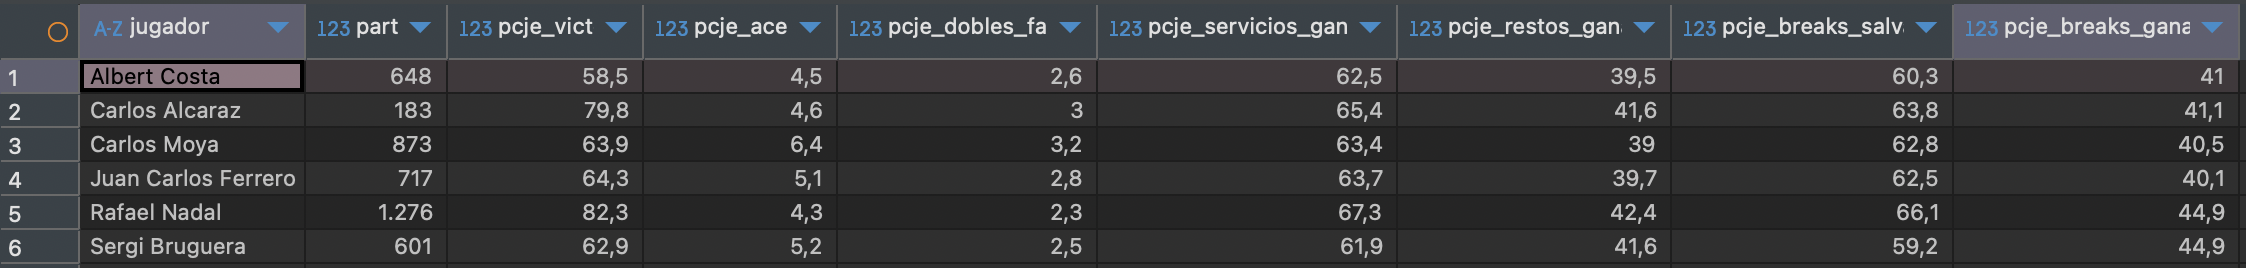
\includegraphics[width=\textwidth]{fotos/q4_com.png}
\caption{Datos agregados en SQL. Tipos compuestos, consulta 4.}
\label{fig:q4_com}
\end{figure}





\subsubsection{Lista los jugadores que fueron derrotados (en algún partido del 2018) por el rival de Rafael Nadal de la primera ronda (R128) de Roland Garros de 2018}

Esta consulta la dividiremos en dos subconsultas, una para obtener el rival de Rafael Nadal en la primera ronda de Roland Garros de 2018 y otra para obtener los jugadores que fueron derrotados por ese rival. Para la primera parte, que solo requiere la tabla \texttt{partidos}, fijamos como condiciones de selección que la ronda sea R128, el nombre del torneo sea Roland Garros y el año sea 2018. Además, el nombre del ganador o perdedor debe ser Rafael, y su apellido Nadal. No explicamos cómo acceder a estos campos porque ya se hizo con anterioridad. Esto devuelve una única fila con el rival de Nadal en este partido concreto, por lo que nos quedamos únicamente con la proyección de su nombre completo (concatenación de \texttt{nombre} y \texttt{apellido}). La tabla resultante la llamaremos \texttt{rival\_nadal}. \\

Para la segunda parte, usaremos el producto cartesiano de \texttt{rival\_nadal} y \texttt{partidos}. Como condiciones de \textit{join} usaremos que el nombre y apellido del rival de Nadal coincida con el nombre y apellidos del ganador de ese partido, que es una columna de tipo compuesto (\texttt{ganador}) a la cual accedemos como en las consultas anteriores. Además, si seleccionamos los partidos disputados en 2018 a través de la fecha, obtenemos un conjunto de tuplas con los partidos ganados por el rival de Nadal en 2018. En la proyección, nos quedamos simplemente con una concatenación del nombre y apellido del perdedor y su país, al que accedemos a través de \texttt{(perdedor).pais.codigo\_iso2}. No haría falta, pero ordenamos el resultado por el nombre del jugador. La consulta y el resultado, que coincide con el esperado, se pueden ver en la figura \ref{fig:q5_com}.

\begin{minted}[frame=single, fontsize=\footnotesize]{sql}
with rival_nadal as (
	select case when (ganador).nombre = 'Rafael' then (perdedor).nombre || ' ' || (perdedor).apellido 
		else (ganador).nombre || ' ' || (ganador).apellido end as jugador
	from partidos 
	where (((ganador).nombre = 'Rafael' and (ganador).apellido = 'Nadal') or 
		((perdedor).nombre = 'Rafael' and(perdedor).apellido = 'Nadal'))
		and ronda = 'R128'
		and (torneo).torneo.nombre = 'Roland Garros'
		and extract(year from fecha) = '2018'
)

select (p.perdedor).nombre || ' ' || (p.perdedor).apellido as jugador, (p.perdedor).pais.codigo_iso2 as pais
from partidos p, rival_nadal rn
where (p.ganador).nombre || ' ' || (p.ganador).apellido = rn.jugador
	and extract(year from p.fecha) = '2018'
order by jugador
\end{minted}


\begin{figure}[H]
\centering
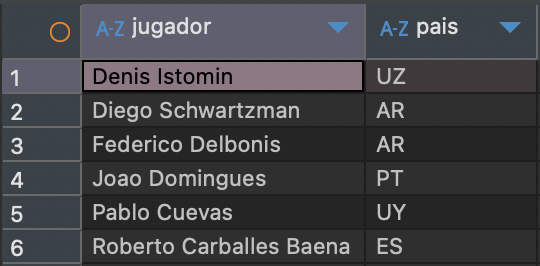
\includegraphics[width=0.35\textwidth]{fotos/q5_com.png}
\caption{Datos agregados en SQL. Tipos compuestos, consulta 5.}
\label{fig:q5_com}
\end{figure}

\subsection{JSON}

A continuación, queremos crear de nuevo una tabla que contenga todos los datos de los partidos (países, torneos, ediciones, partidos, sets y jugadores). Concretamente, está vez debe resolver de forma eficiente las consultas Q2 y Q4. Para mantener orden en nuestra bae de datos, crearemos un nueva esquema \texttt{agregadosJSON} para alojar esta nueva tabla. \\

PostgreSQL proporciona un tipo de datos ``json'' y un conjunto de funciones y operadores que permiten tanto generar documentos JSON a partir de datos relacionales como consultar partes de un documento JSON. Además del tipo ``json'', también se proporciona un tipo más eficiente ``jsonb'', que almacena los documentos en formato binario. Para resolver de forma eficiente las consultas deseadas, nuestra tabla deberá estar orientada a los jugadores, es decir, una tupla para cada jugador con todos sus datos y los partidos que ha jugado. \\

En el caso de JSON (usaremos JSONB), tenemos objetos JSON y agregados de objetos JSON. La creación del esquema de la tabla y la inserción de los datos se realiza mediante la misma consulta, que explicamos a continuación.  \\


Comenzaremos con la tabla \texttt{jugador}, y haremos un \textit{left join} con la tabla \texttt{pais} para obtener los datos del país del jugador. El motivo del \textit{left join} en lugar de un \textit{inner join} lo comentamos en la sección de agregados de tipos compuestos. En el \texttt{where} realizamos un paso crítico para la eficiencia de la consulta: filtramos los jugadores que han participado en algún partido. Para ello, seleccionamos los jugadores cuyo id está en la lista de perdedores o ganadores de algún partido. Debemos hacer esto ya que, de los 60 mil jugadores existentes en la base de datos, unos 58 mil no ganaron ni perdieron ningún partido (según los datos recogidos en nuestra base de datos relacional). \\

Con esto tenemos la tuplas de los partidos jugadores que han participado en algún partido. Al obtener la proyección, haremos que cada tupla tenga los siguientes atributos: 
\begin{itemize}
\item \texttt{jugador}: objeto jsonb con los datos del jugador: id, nombre, apellido, diestro, fecha de nacimiento y altura.
\item \texttt{pais}: objeto jsonb con los datos del país del jugador: código ISO2, código ISO3, código IOC y nombre.
\item \texttt{partidos\_ganados}: agregación de objetos jsonb con los datos de los partidos ganados por el jugador. Cada objeto jsonb será un partido concreto y contendrá los datos del torneo, la fecha, la ronda, el desenlace, el número de partido, el rival, los sets y las estadísticas del jugador y las del rival. \\

La agregación de objetos jsonb se hace mediante subconsultas, por lo que debemos pararnos a explicar la construcción de este agregado más en detalle. Para esta subconsulta partimos de la tabla \texttt{partido}, que denotaremos por el alias \texttt{pg} al estar tratando con los partidos ganados, y realizamos un \textit{left join} con la tabla \texttt{edicion\_torneo} mediante los atributos que definen la FK de la tabla \texttt{partido} y la PK de la tabla \texttt{edicion\_torneo}. A continuación, realizamos un \textit{left join} con la tabla \texttt{torneo} mediante los atributos que definen la FK de la tabla \texttt{edicion\_torneo} y la PK de la tabla \texttt{torneo}. Finalmente, hacemos otro \textit{left join} con la tabla \texttt{pais} mediante el codigo ISO2. Seleccionamos solo los partidos ganados por el jugador que estamos tratando y construimos un objeto jsonb con los datos del torneo, la fecha, la ronda, el desenlace, el número de partido, el rival, los sets y las estadísticas del jugador y las del rival. \\

De estos atributos, \texttt{fecha}, \texttt{ronda}, \texttt{desenlace}, \texttt{num\_partido} y \texttt{perdedor} son directamente obtenidos de la tabla \texttt{partido pg}. Además, \texttt{torneo} es simplemente un objeto jsonb con los datos relativos asa edicion del torneo: nombre, pais (que será un objeto jsonb con los atributos del país que se reflejan en la tabla relacional de \texttt{pais}), fecha, superficie, tamaño y nivel. Las estadísticas de el jugador y del rival son también objetos jsonb que toman los datos estadísticos de la tabla \texttt{partido pg}. \\

Por último, los sets son un agregado de objetos jsonb que se construye mediante una subconsulta que selecciona los sets de un partido concreto. Cada objeto jsonb de este agregado contiene el número de set, los juegos ganados por el jugador, los juegos ganados por el rival y los puntos del tiebreak en caso de que se haya llegado a este. Para hacer la subconsulta descrita nos centramos en la tabla \texttt{sets\_partido}. La unimos con condiciones de \textit{join} a \texttt{partido}, igualando los atributos que componen la clave foránea de \texttt{sets\_partido} con los atributos que componen la clave primaria de \texttt{partido}, seleccionando así solo los sets del partido que estamos tratando. 
\item \texttt{partidos\_perdidos}: este agregado de objetos jsonb lo obtenemos de forma completamente análoga a \texttt{partidos\_ganados}, pero con los partidos perdidos por el jugador.
\end{itemize}


\begin{minted}[frame=single, fontsize=\footnotesize]{sql}
create table tenisjson as
select 
	-- columna 'jugador' como objeto json
	jsonb_build_object(
		'id', j.id, 
		'nombre', j.nombre, 
		'apellido', j.apellido, 
		'diestro', j.diestro, 
		'fecha_nacimiento', j.fecha_nacimiento, 
		'altura', j.altura
	) as jugador,
  -- columna 'pais' como objeto json
	jsonb_build_object(
		'codigo_iso2', p.codigo_iso2, 
		'codigo_iso3', p.codigo_iso3, 
		'codigo_ioc', p.codigo_ioc, 
		'nombre', p.nombre
	) as pais,
  -- columna 'partidos_ganados' como agregado json
	(select jsonb_agg(jsonb_build_object(
		'torneo', jsonb_build_object(
			'nombre', t.nombre, 
			'pais', jsonb_build_object(
				'codigo_iso2', pa.codigo_iso2, 
				'codigo_iso3', pa.codigo_iso3, 
				'codigo_ioc', pa.codigo_ioc, 
				'nombre', pa.nombre), 
			'fecha', et.fecha, 
			'superficie', et.superficie, 
			'tamano', et.tamano, 
			'nivel', et.nivel), 
		'fecha', pg.fecha, 
		'ronda', pg.ronda, 
		'desenlace', pg.desenlace, 
		'num_partido', pg.num_partido, 
		'rival', pg.perdedor, 
		'sets', (select jsonb_agg(
			jsonb_build_object(
				'num_set', sp.num_set, 
				'juegos_ganador', sp.juegos_ganador, 
				'juegos_perdedor', sp.juegos_perdedor, 
				'puntos_tiebreak_perdedor', sp.puntos_tiebreak_perdedor
			)
		) 
		from sets_partido sp 
		where sp.torneo = pg.torneo 
			and sp.fecha = pg.fecha 
			and sp.num_partido = pg.num_partido), 
		'stats', jsonb_build_object(
			'num_aces', pg.num_aces_ganador, 
			'num_dob_faltas', pg.num_dob_faltas_ganador, 
			'num_puntos_servidos', pg.num_ptos_servidos_ganador, 
			'num_primeros_servicios', pg.num_primeros_servicios_ganador, 
			'num_primeros_servicios_ganados', pg.num_primeros_servicios_ganados_ganador, 
			'num_segundos_servicios_ganados', pg.num_segundos_servicios_ganados_ganador, 
			'num_juegos_servidos', pg.num_juegos_servidos_ganador, 
			'num_break_salvados', pg.num_break_salvados_ganador, 
			'num_break_afrontados', pg.num_break_afrontados_ganador
		), 
		'stats_rival', jsonb_build_object(
			'num_aces', pg.num_aces_perdedor, 
			'num_dob_faltas', pg.num_dob_faltas_perdedor, 
			'num_puntos_servidos', pg.num_ptos_servidos_perdedor, 
			'num_primeros_servicios', pg.num_primeros_servicios_perdedor, 
			'num_primeros_servicios_ganados', pg.num_primeros_servicios_ganados_perdedor, 
			'num_segundos_servicios_ganados', pg.num_segundos_servicios_ganados_perdedor, 
			'num_juegos_servidos', pg.num_juegos_servidos_perdedor, 
			'num_break_salvados', pg.num_break_salvados_perdedor, 
			'num_break_afrontados', pg.num_break_afrontados_perdedor
		)
	)) 
	from public.partido pg 
		left join public.edicion_torneo et on pg.torneo = et.torneo and pg.fecha = et.fecha 
		left join public.torneo t on et.torneo = t.id 
		left join public.pais pa on t.pais = pa.codigo_iso2
	where pg.ganador = j.id) as partidos_ganados,
   -- columna 'partidos_perdidos' como json
	(select jsonb_agg(jsonb_build_object(
		'torneo', jsonb_build_object(
			'nombre', t.nombre, 
			'pais', jsonb_build_object(
				'codigo_iso2', pa.codigo_iso2,
				'codigo_iso3', pa.codigo_iso3,
				'codigo_ioc', pa.codigo_ioc,
				'nombre', pa.nombre
			),
			'fecha', et.fecha,
			'superficie', et.superficie,
			'tamano', et.tamano,
			'nivel', et.nivel
		),
		'fecha', pp.fecha,
		'ronda', pp.ronda,
		'desenlace', pp.desenlace,
		'num_partido', pp.num_partido,
		'rival', pp.ganador,
		'sets', (select jsonb_agg(
			jsonb_build_object(
				'num_set', sp.num_set,
				'juegos_ganador', sp.juegos_ganador,
				'juegos_perdedor', sp.juegos_perdedor,
				'puntos_tiebreak_perdedor', sp.puntos_tiebreak_perdedor
			)
		) 
		from sets_partido sp 
		where sp.torneo = pp.torneo 
			and sp.fecha = pp.fecha 
			and sp.num_partido = pp.num_partido),
		'stats', jsonb_build_object(
			'num_aces', pp.num_aces_perdedor,
			'num_dob_faltas', pp.num_dob_faltas_perdedor,
			'num_puntos_servidos', pp.num_ptos_servidos_perdedor,
			'num_primeros_servicios', pp.num_primeros_servicios_perdedor,
			'num_primeros_servicios_ganados', pp.num_primeros_servicios_ganados_perdedor,
			'num_segundos_servicios_ganados', pp.num_segundos_servicios_ganados_perdedor,
			'num_juegos_servidos', pp.num_juegos_servidos_perdedor,
			'num_break_salvados', pp.num_break_salvados_perdedor,
			'num_break_afrontados', pp.num_break_afrontados_perdedor
		),
		'stats_rival', jsonb_build_object(
			'num_aces', pp.num_aces_ganador,
			'num_dob_faltas', pp.num_dob_faltas_ganador,
			'num_puntos_servidos', pp.num_ptos_servidos_ganador,
			'num_primeros_servicios', pp.num_primeros_servicios_ganador,
			'num_primeros_servicios_ganados', pp.num_primeros_servicios_ganados_ganador,
			'num_segundos_servicios_ganados', pp.num_segundos_servicios_ganados_ganador,
			'num_juegos_servidos', pp.num_juegos_servidos_ganador,
			'num_break_salvados', pp.num_break_salvados_ganador,
			'num_break_afrontados', pp.num_break_afrontados_ganador
		)
	)) 
	from public.partido pp
		left join public.edicion_torneo et on pp.torneo = et.torneo and pp.fecha = et.fecha
		left join public.torneo t on et.torneo = t.id
		left join public.pais pa on t.pais = pa.codigo_iso2
	where pp.perdedor = j.id) as partidos_perdidos
from public.jugador j
	left join public.pais p on j.pais = p.codigo_iso2
where j.id in (select perdedor from public.partido)
	or j.id in (select ganador from public.partido)
\end{minted}

\noindent Antes de comenzar con las consultas, comentamos los aspectos clave:
\begin{itemize}
\item Para acceder a un valor como un objeto jsonb completo, usamos la notación ->. 
\item Para acceder a un valor como un texto, usamos la notación ->>.
\item Para acceder a elementos de un array jsonb, debemos usar la función \texttt{jsonb\_array\_elements(nombre\_array)}. Esto extrae los elementos y los asigna a registros independientes. Esto es similar a la función \texttt{unnest} que usamos en los arrays de PostgreSQL y, del mismo modo, se puede asignar un alias a cada elemento del array.
\end{itemize}

Así, por ejemplo, para acceder al nombre de un torneo, con la estrucura que creamos, debemos desagregar al agregado jsonb `partidos ganados' con \texttt{jsonb\_array\_elements(partidos\_ganados)} y acceder al campo `torneo' con -> (ya que es un objeto jsonb) y al campo `nombre' con ->>. Así, si previamente asignamos a \texttt{jsonb\_array\_elements(partidos\_ganados)} el alias \texttt{partidos(pg)}, cada elemento del array se denotará por ``pg'', y podremos acceder al nombre del torneo como \texttt{pg} -> \texttt{`torneo'} ->> \texttt{`nombre'}. 

\subsubsection{Muestra todos los ganadores del torneo ``Wimbledon'' (Nombre apellidos y año). Ordena el resultado por año.}

El ejemplo anterior nos resulta útil para resolver esta consulta (curiosamente usa uno de los atributos que necesitamos\dots). Para esta consulta partimos del producto cartesiano de la tabla \texttt{tenisjson} con la función \texttt{jsonb\_array\_elements(partidos\_ganados)} para extraer los elementos jsonb de partidos ganados. Con esto, estamos generando tuplas que no nos son de utilidad para la consulta, así que debemos hacer una selección en el \texttt{where} para quedarnos solo con los partidos finales de Wimbledon. Para ello, seleccionamos los partidos finales (a ronda accedemos desde ``pg'' con ->>, ya que queremos el resultado como texto) cuyo torneo tenga nombre ``Wimbledon'' (aquí tenemos el ejemplo anterior). A continuación, seleccionamos el nombre y apellido del jugador y el año del torneo como atributos de texto. Aquí hay una sutileza a tener en cuenta: como estamos obteniendo la fecha en formato texto al usar ->>, debemos convertirla a tipo \texttt{date} con \texttt{::date} antes de usar el \texttt{extract(year \dots)} que venimos usando durante todo el trabajo. Finalmente, ordenamos el resultado por año. La consulta se muestra a continuación, y el resultado es el esperado (figura \ref{fig:q1_json})

\begin{minted}[frame=single, fontsize=\footnotesize]{sql}
select tj.jugador ->> 'nombre' as nombre, 
    tj.jugador ->> 'apellido' as apellido, 
    extract(year from (pg ->> 'fecha')::date) as ano
from tenisjson tj, jsonb_array_elements(partidos_ganados) as partidos(pg)
where pg ->> 'ronda' = 'F' 
    and pg -> 'torneo' ->> 'nombre' = 'Wimbledon'
order by ano
\end{minted}

\begin{figure}[H]
\centering
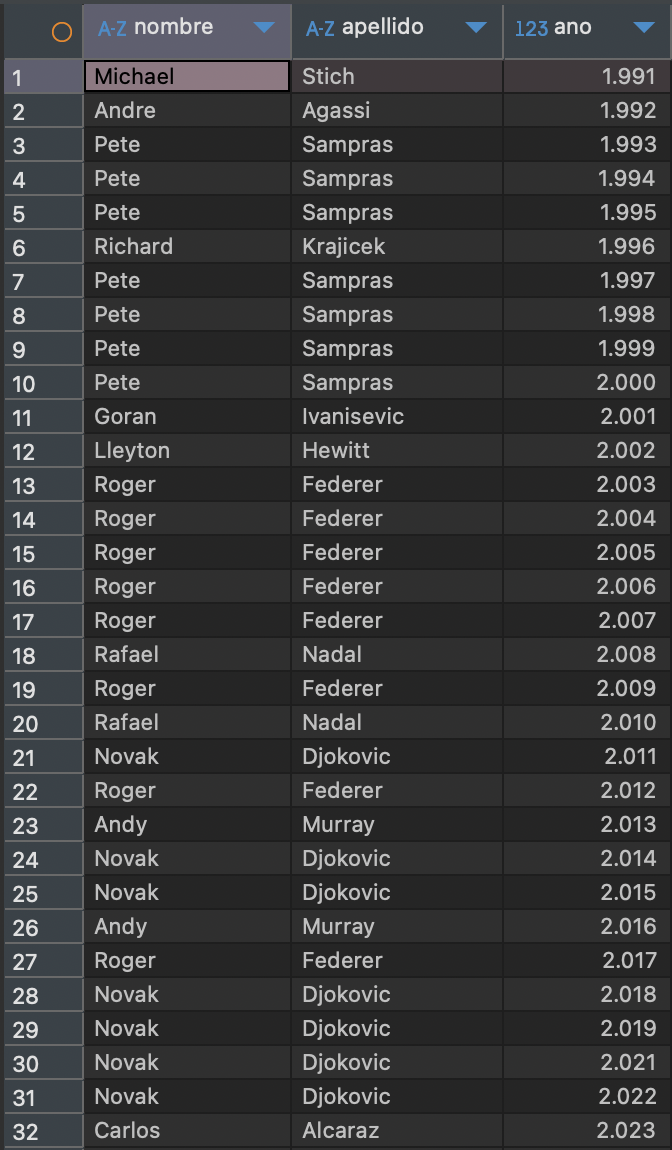
\includegraphics[height=0.4\textheight]{fotos/q1_json.png}
\caption{Datos agregados en SQL. Tipo JSON, consulta 1.}
\label{fig:q1_json}
\end{figure}



\subsubsection{Muestra los años en los que Roger Federer ganó algún torneo de nivel Gran Slam (G) o Master 1000 (M). Para cada año, muestra el número de torneos y lista sus nombres (ordenados por la fecha de celebración). Ordena el resultado por el año}

Para esta consulta partimos del mismo punto que para la anterior: el producto cartesiano de la tabla \texttt{tenisjson} con la función \texttt{jsonb\_array\_elements(partidos\_ganados)}. Esta vez, la selección es más específica: queremos los partidos finales (accedemos en \texttt{ronda} como texto) de torneos Grand Slam o Master 1000 (accedemos como texto con \texttt{`torneo'} ->> \texttt{`nivel'}), donde el ganador sea Roger Federer (accedemos al nombre y apellido como texto del jugador desde \texttt{jugador}). Esto nos da una tupla para cada final ganada por Federer, por lo que para nuestro resultado debemos hacer un \texttt{group by} por año. Así, tenemos una tupla para cada año. \\

Finalmente, obtenemos la proyección usando el año del torneo (al cual accedemos como en la anterior consulta), el conteo de los torneos (usamos \texttt{count(distinct)} sobre el nombre de los torneos para evitar contar repetidos) y los nombres de los torneos (usamos \texttt{string\_agg} para concatenar los nombres de los torneos, ordenados por fecha de celebración). Ordenamos el resultado final por año en orden ascendente. La consulta se muestra a continuación, y el resultado es el esperado (figura \ref{fig:q2_json})

\begin{minted}[frame=single, fontsize=\footnotesize]{sql}
select extract(year from (pg -> 'torneo' ->> 'fecha')::date) as ano,
    count(distinct pg -> 'torneo'->>'nombre') as numero_torneos,
    string_agg(pg -> 'torneo'->>'nombre', ', ' order by pg -> 'torneo' ->> 'fecha') as torneos
from tenisjson tj, jsonb_array_elements(partidos_ganados) as partidos(pg)
where tj.jugador ->> 'nombre' = 'Roger'
    and tj.jugador ->> 'apellido' = 'Federer'
    and pg ->> 'ronda' = 'F'
    and pg -> 'torneo'->>'nivel' in ('G', 'M')
group by ano
order by ano
\end{minted}

\begin{figure}[H]
\centering
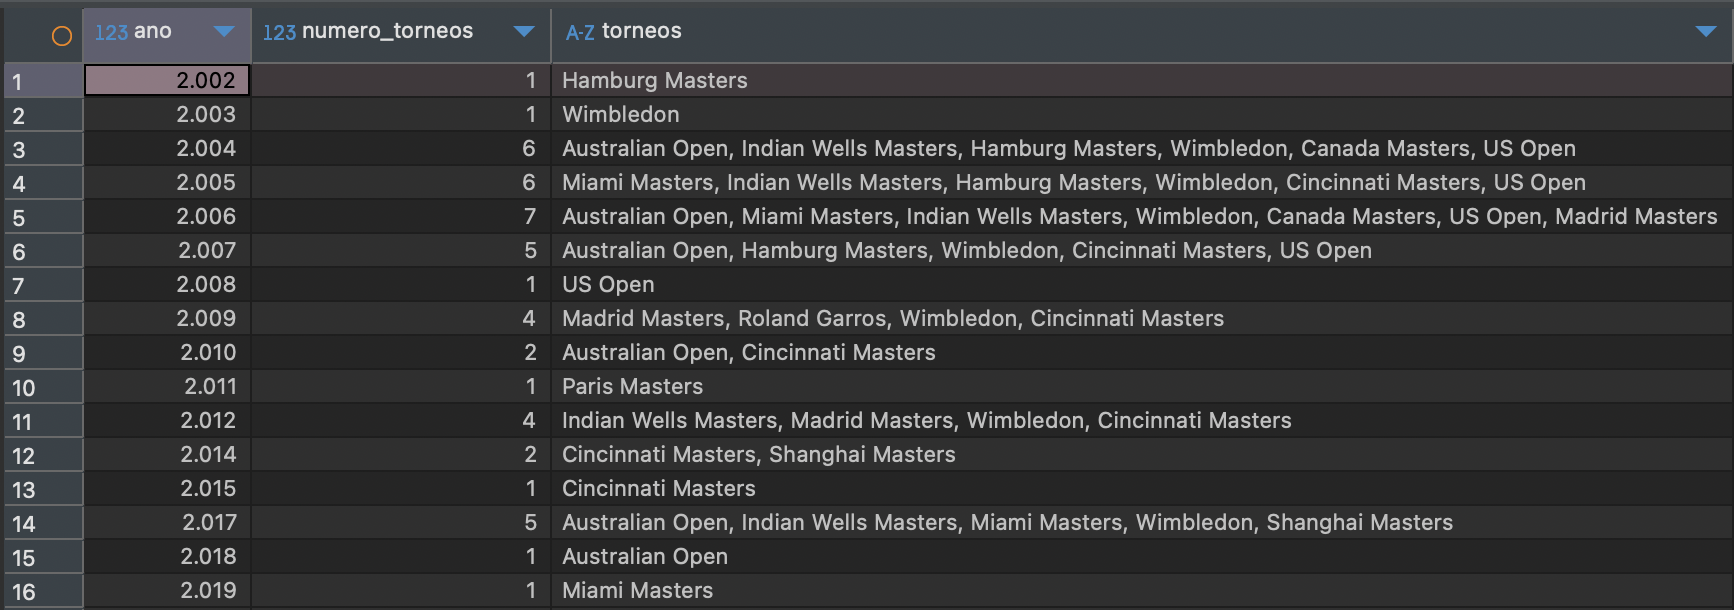
\includegraphics[width=0.8\textwidth]{fotos/q2_json.png}
\caption{Datos agregados en SQL. Tipo JSON, consulta 2.}
\label{fig:q2_json}
\end{figure}



\subsubsection{Muestra los partidos de semifinales (ronda='SF') y final (ronda = 'F') del torneo de "Roland Garros" del 2018. Para cada partido muestra la ronda, el tipo de desenlace, el nombre y apellidos del ganador y el nombre y apellidos del perdedor y el resultado con el número de juegos del ganador y del perdedor en cada set, y opcionalmente en paréntesis el número de juegos del perdedor en el tie break}

Para esta consulta, partimos del producto cartesiano de la tabla \texttt{tenisjson} con las funciones \texttt{jsonb\_array\_el-}\\\texttt{ements(partidos\_ganados)} y \texttt{jsonb\_array\_elements(pg} -> \texttt{`sets')} para extraer los elementos jsonb de partidos ganados y extraer los elementos del objeto jsonb `sets', que designaremos por un alias. Esta vez estamos considerando dos veces la tabla \texttt{tenisjson}, ya que necesitamos estadísticas del ganador y del perdedor. Con esto tenemos de nuevo un exceso de filas debido al producto cartesiano, por lo que seleccionamos los partidos de semifinales y finales de Roland Garros 2018 (accedemos a la ronda, la fecha y al nombre del torneo como texto). Además, seleccionamos solo las tuplas donde el \texttt{id} del jugador rival coincida con el \texttt{id} del jugador de la segunda tabla \texttt{tenisjson} que consideramos. Con todo esto, tenemos una tupla para cada set de cada partido de semifinales y finales de Roland Garros 2018. Como esto no es lo que queremos, agrupamos por \texttt{ronda}, \texttt{desenlace} y nombre y apellidos del ganador y del perdedor. \\

Con todo esto tenemos simplemente una tupla por cada partido (3, 2 para semifinales y una para final). Para la proyección, seleccionamos la ronda, el desenlace, el nombre y apellidos del ganador y del perdedor como texto (nótese que al concatenar nombre y apellidos debemos hacer la conversión explícita de los atributos a texto) y el resultado, que se construye concatenando el número de juegos del ganador y del perdedor en cada set, y opcionalmente el número de juegos del perdedor en el tie break (si este existe). La consulta se muestra a continuación, y el resultado es el esperado (figura \ref{fig:q3_json})

\begin{minted}[frame=single, fontsize=\footnotesize]{sql}
select pg ->> 'ronda' as ronda, pg ->> 'desenlace' as desenlace, 
	(tj.jugador ->> 'nombre')::text || ' ' || (tj.jugador ->> 'apellido')::text as ganador, 
	(tjr.jugador ->> 'nombre')::text || ' ' || (tjr.jugador ->> 'apellido')::text as perdedor, 
	string_agg((s ->> 'juegos_ganador')::text || '-' || (s ->> 'juegos_perdedor')::text || 
		case when s ->> 'puntos_tiebreak_perdedor' is not null 
			then '(' || (s ->> 'puntos_tiebreak_perdedor')::text || ')' 
			else '' end, ', ' order by s ->> 'num_set') as resultado
from tenisjson tj, jsonb_array_elements(tj.partidos_ganados) as partidos(pg), 
	jsonb_array_elements(pg -> 'sets') as setss(s), tenisjson tjr
where pg ->'torneo' ->> 'nombre' = 'Roland Garros'
    and extract(year from (pg ->> 'fecha')::date) = 2018
    and pg ->> 'ronda' in ('SF', 'F')
    and tjr.jugador->>'id' = pg ->> 'rival'
group by pg ->> 'ronda', pg ->> 'desenlace', 
	tj.jugador ->> 'nombre', tj.jugador ->> 'apellido', 
	tjr.jugador ->> 'nombre', tjr.jugador ->> 'apellido'
\end{minted}

\begin{figure}[H]
\centering
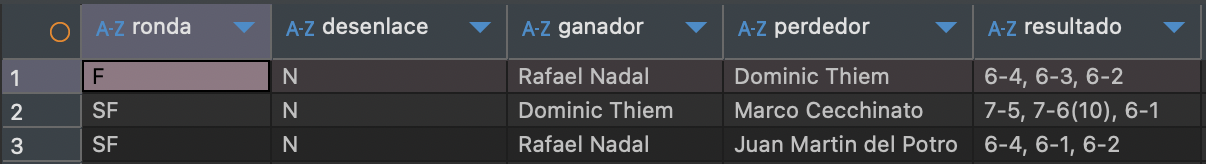
\includegraphics[width=0.7\textwidth]{fotos/q3_json.png}
\caption{Datos agregados en SQL. Tipo JSON, consulta 3.}
\label{fig:q3_json}
\end{figure}



\subsubsection{Muestra la lista de jugadores españoles (ES) que ganaron algún torneo de nivel Gran Slam (G). Para cada jugador muestra los siguientes datos resumen de todos sus partidos: número de partidos jugados, porcentaje de victorias, porcentaje de aces, porcentaje de dobles faltas, porcentaje de servicios ganados, porcentaje de restos ganados, porcentaje de break points salvados (de los sufridos en contra), porcentaje de break points ganados (de los provocados a favor)}


Como anteriormente, se dividirá esta consulta en dos: una primera parte que selecciona los jugadores españoles que ganaron algún torneo de nivel Gran Slam y una segunda parte que calcula los datos resumen de todos sus partidos. \\

Para la primera parte, partimos del producto cartesiano de la tabla \texttt{tenisjson} con la función \texttt{jsonb\_array\_el-}\\\texttt{ements(partidos\_ganados)} para extraer los elementos jsonb de partidos ganados. Seleccionamos los jugadores españoles (accedemos al código ISO2 del país como texto) que ganaron algún torneo de nivel Gran Slam (accedemos a la ronda y al nivel del torneo como texto). Con esto, tenemos una tupla para cada partido final ganado por un jugador español en un torneo de nivel Gran Slam. En la proyección, nos quedamos con el \texttt{id} y el nombre y apellido del jugador, usando \texttt{distinct} para evitar duplicados. \\

Para la segunda parte, partimos del producto cartesiano de la tablade jugadores españoles con \texttt{tenisjson} y con la función \texttt{jsonb\_array\_elements(tj.partidos\_ganados)} para extraer los elementos jsonb de partidos ganados. Seleccionamos en el \texttt{where} los partidos en los que los jugadores españoles antes diferenciados aparece, tanto como ganadores como rivales. Con esto, tenemos una tupla para cada partido jugado por un jugador español (que haya ganado un Grand Slam). Antes de hacer la proyección, agrupamos por jugador para tener una tupla para cada jugador. \\

La proyección para obtener las estadísticas del jugador es conceptualmente igual a lo que ya hicimos en esta consulta para el modelo relacional y para el de tipos compuestos. Solo tenemos que tener en cuenta que los valores que queremos están en el objeto jsonb `stats' o en `stats\_rival' de cada partido (es decir, accedemos con ->). Una vez dentro de estos, accedemos con normalidad a las estadísticas que queramos en formato texto con ->>. La consulta se muestra a continuación, y el resultado es el esperado (figura \ref{fig:q4_json})

\begin{minted}[frame=single, fontsize=\footnotesize]{sql}
with jugadores_espanoles_ganadores as (
    select distinct (tj.jugador ->> 'id')::integer as id_jugador, 
    	(tj.jugador ->> 'nombre')::text || ' ' || (tj.jugador ->> 'apellido')::text as jugador
    from tenisjson tj, jsonb_array_elements(partidos_ganados) as partidos(pg)
    where tj.pais ->> 'codigo_iso2' = 'ES'
        and pg ->> 'ronda' = 'F'
        and pg -> 'torneo' ->> 'nivel' = 'G'
)

select jeg.jugador,
    count(*) as partidos,
    round(100.0 * count(case when pg ->> 'rival' = jeg.id_jugador::text then null else 1 end)::numeric / 
	count(*), 1) as pcje_victorias,
    round(100.0 * sum(case when pg ->> 'rival' = jeg.id_jugador::text 
    	then (pg -> 'stats_rival' ->> 'num_aces')::numeric 
    	else (pg -> 'stats' ->> 'num_aces')::numeric end) / 
    	nullif(sum(case when pg ->> 'rival' = jeg.id_jugador::text 
    		then (pg -> 'stats_rival' ->> 'num_puntos_servidos')::numeric 
    		else (pg->'stats'->>'num_puntos_servidos')::numeric end), 0), 1) as pcje_aces,
    round(100.0 * sum(case when pg ->> 'rival' = jeg.id_jugador::text 
    	then (pg -> 'stats_rival' ->> 'num_dob_faltas')::numeric 
    	else (pg -> 'stats' ->> 'num_dob_faltas')::numeric end) / 
    	nullif(sum(case when pg ->> 'rival' = jeg.id_jugador::text 
    		then (pg -> 'stats_rival' ->> 'num_puntos_servidos')::numeric 
    		else (pg -> 'stats' ->> 'num_puntos_servidos')::numeric end), 0), 1) 
			as pcje_dobles_faltas,
    round(100.0 * sum(case when pg ->> 'rival' = jeg.id_jugador::text 
    	then (pg -> 'stats_rival' ->> 'num_primeros_servicios_ganados')::numeric + 
		(pg -> 'stats_rival' ->> 'num_segundos_servicios_ganados')::numeric 
    	else (pg -> 'stats' ->> 'num_primeros_servicios_ganados')::numeric + 
		(pg -> 'stats' ->> 'num_segundos_servicios_ganados')::numeric end) / 
    	nullif(sum(case when pg ->> 'rival' = jeg.id_jugador::text 
    		then (pg -> 'stats_rival' ->> 'num_puntos_servidos')::numeric 
    		else (pg -> 'stats' ->> 'num_puntos_servidos')::numeric end), 0), 1) 
			as pcje_servicios_ganados,
    round(100.0 * sum(case when pg ->> 'rival' = jeg.id_jugador::text 
    	then (pg -> 'stats' ->> 'num_puntos_servidos')::numeric - 
		(pg -> 'stats' ->> 'num_primeros_servicios_ganados')::numeric - 
    		 (pg -> 'stats' ->> 'num_segundos_servicios_ganados')::numeric 
    	else (pg -> 'stats_rival' ->> 'num_puntos_servidos')::numeric - 
		(pg -> 'stats_rival' ->> 'num_primeros_servicios_ganados')::numeric - 
    		 (pg -> 'stats_rival' ->> 'num_segundos_servicios_ganados')::numeric end) / 	
    	nullif(sum(case when pg ->> 'rival' = jeg.id_jugador::text 
    		then (pg -> 'stats' ->> 'num_puntos_servidos')::numeric 
    		else (pg -> 'stats_rival' ->> 'num_puntos_servidos')::numeric end), 0), 1) 
			as pcje_restos_ganados,
    round(100.0 * sum(case when pg ->> 'rival' = jeg.id_jugador::text 
    	then (pg->'stats_rival'->>'num_break_salvados')::numeric 
    	else (pg -> 'stats' ->> 'num_break_salvados')::numeric end) / 
    	nullif(sum(case when pg ->> 'rival' = jeg.id_jugador::text 
    		then (pg -> 'stats_rival' ->> 'num_break_afrontados')::numeric 
    		else (pg -> 'stats' ->> 'num_break_afrontados')::numeric end), 0), 1) 
			as pcje_breaks_salvados,
    round(100.0 * sum(case when pg ->> 'rival' = jeg.id_jugador::text 
    	then (pg -> 'stats' ->> 'num_break_afrontados')::numeric - 
		(pg -> 'stats' ->> 'num_break_salvados')::numeric
    	else (pg -> 'stats_rival' ->> 'num_break_afrontados')::numeric - 
		(pg -> 'stats_rival' ->> 'num_break_salvados')::numeric end) / 
    	nullif(sum(case when pg ->> 'rival' = jeg.id_jugador::text 
    		then (pg -> 'stats' ->> 'num_break_afrontados')::numeric 
    		else (pg -> 'stats_rival' ->> 'num_break_afrontados')::numeric end), 0), 1) 
			as pcje_breaks_ganados
from jugadores_espanoles_ganadores jeg, tenisjson tj, 
	jsonb_array_elements(tj.partidos_ganados) as partidos(pg)
where (tj.jugador ->> 'id')::integer = jeg.id_jugador 
	or pg ->> 'rival' = jeg.id_jugador::text
group by jeg.jugador
\end{minted}


\begin{figure}[H]
\centering
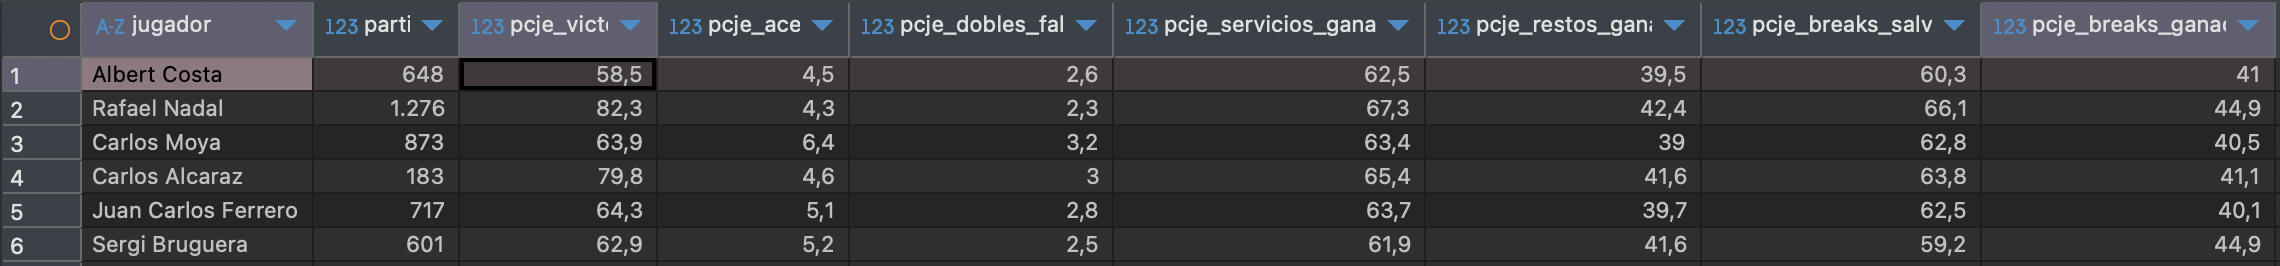
\includegraphics[width=\textwidth]{fotos/q4_json.png}
\caption{Datos agregados en SQL. Tipo JSON, consulta 4.}
\label{fig:q4_json}
\end{figure}


\subsubsection{Lista los jugadores que fueron derrotados (en algún partido del 2018) por el rival de Rafael Nadal de la primera ronda (R128) de Roland Garros de 2018}

Esta consulta la dividiremos en dos subconsultas: una que selecciona el rival de Rafael Nadal en la primera ronda de Roland Garros 2018 y otra que selecciona los jugadores que fueron derrotados por este rival en algún partido del 2018. \\

Para la primera parte, partimos del producto cartesiano de la tabla \texttt{tenisjson} (por duplicado, para discernir entre ganador y perdedor) con la función \texttt{jsonb\_array\_elements(partidos\_ganados)} para extraer los elementos jsonb de partidos ganados. Seleccionamos solo las tuplas que nos interesan: 
\begin{itemize}
\item El nombre torneo debe ser Roland Garros.
\item La ronda debe ser R128.
\item El año de la fecha debe ser del 2018.
\item El nombre y apellido de un jugador debe ser Rafael Nadal, respectivamente. Como no sabemos si ganó o perdió, debemos considerar ambos casos: si es ganador (buscando en la tabla \texttt{tenisjson tj}), o si es perdedor (buscando en la tabla \texttt{tenisjson} con el alias \texttt{tjr}).
\end{itemize}

Con esto, tenemos un única tupla con el rival de Rafael Nadal en la primera ronda de Roland Garros 2018. Proyectamos para obtener el \texttt{id} del jugador rival y el nombre y apellido del jugador, considerando que, cuando el ganador sea Nadal, debemos obtener el rival desde \texttt{tjr}, mientras que en caso contrario, debemos obtener al rival desde \texttt{tj}. No explicamos como acceder a los atributos concretos ya que ya se ha hecho con anterioridad para estos parámetros concretos. El resultado lo guardamos en una tabla temporal \texttt{rival\_nadal}. \\

Para la segunda parte, partimos del producto cartesiano de la tabla anterior con \texttt{tenisjson} y con la función \texttt{jsonb\_array\_elements(tj.partidos\_perdidos)} para extraer los elementos jsonb de partidos perdidos. En el \texttt{where} hacemos una selección de las tuplas para las cuales el \texttt{id} del rival (es decir, el ganador) figure como el del rival de Nadal que encontramos antes. Además, seleccionamos solo los partidos del 2018. Con esto, tenemos una tupla para cada partido ganado por este jugador en el año 2018 (no hay repetidos). En la proyección, seleccionamos simplemente el nombre y apellido del jugador (que concatenamos al seleccionar como texto con ->>) y el código ISO2 del país. La consulta se muestra a continuación, y el resultado es el esperado (figura \ref{fig:q5_json})

\begin{minted}[frame=single, fontsize=\footnotesize]{sql}
with rival_nadal as (
	select case when tj.jugador ->> 'nombre' = 'Rafael' 
			then (pg ->> 'rival')::integer  
			else (tj.jugador ->> 'id')::integer end as id_jugador,
		case when tj.jugador ->> 'nombre' = 'Rafael' 
			then (tjr.jugador ->> 'nombre')::text || ' ' || (tjr.jugador ->> 'apellido')::text 
			else (tj.jugador ->> 'nombre')::text || ' ' || (tj.jugador ->> 'apellido')::text 
			end as jugador
	from tenisjson tj, jsonb_array_elements(tj.partidos_ganados) as partidos(pg), tenisjson tjr
    where pg -> 'torneo' ->> 'nombre' = 'Roland Garros' 
    	and pg ->> 'ronda' = 'R128'
		and extract(year from (pg ->> 'fecha')::date) = 2018
        and tjr.jugador->>'id' = pg ->> 'rival'
        and ((tj.jugador ->> 'nombre' = 'Rafael' and tj.jugador ->> 'apellido' = 'Nadal') 
        	or (tjr.jugador ->> 'nombre' = 'Rafael' and tjr.jugador ->> 'apellido' = 'Nadal'))
)

select tj.jugador->>'nombre' || ' ' || (tj.jugador->>'apellido')::text as jugador, 
	tj.pais->>'codigo_iso2' as pais
from rival_nadal rn, tenisjson tj, jsonb_array_elements(tj.partidos_perdidos) as partidos(pg)
where rn.id_jugador = (pg->>'rival')::integer 
	and extract(year from (pg->>'fecha')::date) = 2018
\end{minted}

\begin{figure}[H]
\centering
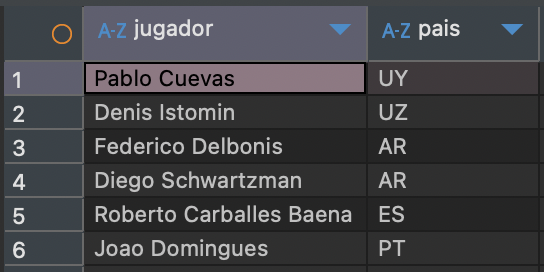
\includegraphics[width=0.35\textwidth]{fotos/q5_json.png}
\caption{Datos agregados en SQL. Tipo JSON, consulta 5.}
\label{fig:q5_json}
\end{figure}

\section{Bases de datos distribuidas con SQL (CITUS Data)}

\subsubsection{Muestra todos los ganadores del torneo ``Wimbledon'' (Nombre apellidos y año). Ordena el resultado por año.}

\begin{lstlisting}[language=SQL]
-- Q1
\end{lstlisting}





\subsubsection{Muestra los años en los que Roger Federer ganó algún torneo de nivel Gran Slam (G) o Master 1000 (M). Para cada año, muestra el número de torneos y lista sus nombres (ordenados por la fecha de celebración). Ordena el resultado por el año}

\begin{lstlisting}[language=SQL]
-- Q2
\end{lstlisting}





\subsubsection{Muestra los partidos de semifinales (ronda='SF') y final (ronda = 'F') del torneo de "Roland Garros" del 2018. Para cada partido muestra la ronda, el tipo de desenlace, el nombre y apellidos del ganador y el nombre y apellidos del perdedor y el resultado con el número de juegos del ganador y del perdedor en cada set, y opcionalmente en paréntesis el número de juegos del perdedor en el tie break}

\begin{lstlisting}[language=SQL]
-- Q3
\end{lstlisting}





\subsubsection{Muestra la lista de jugadores españoles (ES) que ganaron algún torneo de nivel Gran Slam (G). Para cada jugador muestra los siguientes datos resumen de todos sus partidos: número de partidos jugados, porcentaje de victorias, porcentaje de aces, porcentaje de dobles faltas, porcentaje de servicios ganados, porcentaje de restos ganados, porcentaje de break points salvados (de los sufridos en contra), porcentaje de break points ganados (de los provocados a favor)}

\begin{lstlisting}[language=SQL]
-- Q4
\end{lstlisting}





\subsubsection{Lista los jugadores que fueron derrotados (en algún partido del 2018) por el rival de Rafael Nadal de la primera ronda (R128) de Roland Garros de 2018}

\begin{lstlisting}[language=SQL]
-- Q5
\end{lstlisting}
\section{Bases de datos NoSQL: Documentales (MongoDB)}

Para crear el \textit{cluster} de MongoDB propuesto, también emplearemos las máquinas reales del apartado de Citus. Para ello, necesitaremos 3 nodos; en cada uno se ejecutarán 4 procesos \texttt{mongod} y un proceso \texttt{mongos}. Primero, es necesario instalar y configurar MongoDB.

\subsection*{Instalación y Configuración}

Mediante el siguiente \textit{script Bash}, podemos instalar la versión 6.0 del paquete \texttt{mongo-org} en nuestras máquinas. Un detalle importante de esta versión con respecto a la versión instalada en las máquinas virtuales es que el comando \texttt{mongo} ha sido renombrado a \texttt{mongosh}.

\begin{minted}[frame=single, fontsize=\footnotesize]{bash}
#!/bin/bash

# run from local with: ssh user@host 'bash -s' < <path_to_this_file>

# Importar la clave de mongo al llavero del sistema operativo
wget -qO - https://www.mongodb.org/static/pgp/server-6.0.asc |  gpg --dearmor | \
sudo tee /usr/share/keyrings/mongodb.gpg > /dev/null

# Actualizar el repositorio de apt para incluir mongo-org
echo "deb [ arch=amd64,arm64 signed-by=/usr/share/keyrings/mongodb.gpg ]" \
"https://repo.mongodb.org/apt/ubuntu jammy/mongodb-org/6.0 multiverse" | \
sudo tee /etc/apt/sources.list.d/mongodb-org-6.0.list

# Actualizar el controlador de paquetes del sistema
sudo apt update

# Instalar mongo
sudo apt install -y mongodb-org

# Mostrar versiones instaladas
mongod --version
mongosh --version

# Reiniciar el sistema
sudo reboot
\end{minted}

Para facilitar el manejo de direcciones IP, podemos añadir un alias para las distintas IP de las máquinas en el archivo \texttt{\$HOME/etc/hosts}, lo cual nos permitirá hacer referencia a otros nodos de una forma mucho más cómoda.

\begin{minted}[frame=single, fontsize=\footnotesize]{bash}
#!/bin/bash

HOSTS=(
    "51.210.241.66   ovh1"
    "51.210.241.239  ovh2"
    "51.210.241.207  ovh3"
)

# Añadir pareja {ip: alias} a /etc/hosts si no existen
for ENTRY in "${HOSTS[@]}"; do
  IP=$(echo "${ENTRY}" | awk '{print $1}')
  HOSTNAME=$(echo "${ENTRY}" | awk '{print $2}')
  
  if grep -q "${IP}" /etc/hosts; then
    echo "Entry '${ENTRY}' already exists in /etc/hosts. Skipping."
  else
    echo "Adding '${ENTRY}' to /etc/hosts"
    echo "${ENTRY}" | sudo tee -a /etc/hosts > /dev/null
  fi
done

tail /etc/hosts -n 5
\end{minted}

\subsection*{Lanzamiento de los Procesos de MongoDB}

Para crear nuestro \textit{cluster}, es necesario lanzar un total de 4 procesos \texttt{mongod} y un proceso \texttt{mongos} en cada nodo. Cada proceso tendrá una configuración específica según su rol en el \textit{cluster}. A continuación, se describen los detalles de estos procesos:

\begin{itemize}
    \item \textbf{1 proceso de configuración (\texttt{configsrv})}: Este proceso \texttt{mongod} actúa como el servidor de configuración del \textit{cluster}. Su rol es almacenar los metadatos del \textit{cluster}, como el mapeo de fragmentos y la información de distribución de datos.
    \item \textbf{3 procesos de fragmentos (\texttt{shardsvr})}: Estos procesos \texttt{mongod} se encargan de almacenar los datos reales del \textit{cluster}. Cada uno representa un fragmento diferente del conjunto de datos. Cada fragmento se configurará como un conjunto de réplicas para mejorar la redundancia y disponibilidad.
    \item \textbf{1 proceso de enrutamiento (\texttt{mongos})}: Este proceso actúa como el enrutador del \textit{cluster}. Es el encargado de recibir las solicitudes de los clientes y dirigirlas a los fragmentos correspondientes. Debe configurarse para conectarse a los servidores de configuración (\texttt{configsvr}) y proporciona un punto de entrada único para las operaciones del cliente, ocultando la complejidad interna del \textit{cluster}.
\end{itemize}

Para lanzar estos procesos, podemos hacerlo desde la terminal especificando las distintas opciones como argumentos, o podemos crear archivos de configuración específicos para cada proceso. Optamos por la segunda vía, definiendo los siguientes archivos de configuración: \\

\noindent \textbf{Archivo de Configuración para el Config Server}

\begin{minted}[frame=single, fontsize=\footnotesize]{yaml}
sharding:
  clusterRole: configsvr
  
replication:
  replSetName: rsConfServer

storage:
  dbPath: /home/ubuntu/dbMongo/rsConfServer

systemLog:
  destination: file
  logAppend: true
  path: /home/ubuntu/dbMongo/rsConfServer/mongod.log

net:
  port: 27010
  bindIp: 0.0.0.0

processManagement:
  timeZoneInfo: /usr/share/zoneinfo
  fork: true

security:
  keyFile: /home/ubuntu/mongo_keyfile
  authorization: enabled
\end{minted}
\newpage 

\noindent \textbf{Archivo de Configuración para los Shards:} para cada uno de los 3 \textit{shards}, el archivo de configuración sería el siguiente. Solo cambia el nombre del conjunto de réplicas (\texttt{replSetName}), las rutas a los directorios donde se guardarán los datos, los \textit{logs} y el puerto (\texttt{net.port}) para cada \textit{shard}.

\begin{minted}[frame=single, fontsize=\footnotesize]{yaml}
sharding:
  clusterRole: shardsvr
  
replication:
  replSetName: rsShard{1|2|3}

storage:
  dbPath: /home/ubuntu/dbMongo/rsShard{1|2|3}

systemLog:
  destination: file
  logAppend: true
  path: /home/ubuntu/dbMongo/rsShard{1|2|3}/mongod.log

net:
  port: {27011 | 27012 | 27013}
  bindIp: 0.0.0.0

processManagement:
  timeZoneInfo: /usr/share/zoneinfo
  fork: true

security:
  keyFile: /home/ubuntu/mongo_keyfile
  authorization: enabled
\end{minted}

\noindent \textbf{Archivo de Configuración para el Proceso Mongos} 

\begin{minted}[frame=single, fontsize=\footnotesize]{yaml}
sharding:
  configDB: rsConfServer/ovh1:27010,ovh2:27010,ovh3:27010

processManagement:
  timeZoneInfo: /usr/share/zoneinfo
  fork: true

security:
  keyFile: /home/ubuntu/mongo_keyfile

systemLog:
  destination: file
  logAppend: true
  path: /home/ubuntu/dbMongo/mongos/mongod.log

net:
  port: 27017
  bindIp: 0.0.0.0
\end{minted}

\noindent A continuación, se explican las diferentes opciones de configuración:

\begin{enumerate}
    \item \textbf{sharding.clusterRole}: 
    \begin{itemize}
        \item Define el rol de cada nodo dentro del \textit{cluster} de \textit{sharding}. Puede ser \texttt{configsvr} (servidor de configuración) o \texttt{shardsvr} (shard). El proceso \texttt{mongos} no tiene esta opción.
    \end{itemize}
    \item \textbf{replication.replSetName}: 
    \begin{itemize}
        \item Especifica el nombre del conjunto de réplicas para los nodos de replicación. Los nodos de los \textit{shards} y el \texttt{config server} estarán en conjuntos de réplicas, lo que garantiza la disponibilidad y la redundancia de los datos.
    \end{itemize}
    \item \textbf{storage.dbPath}: 
    \begin{itemize}
        \item Define la ruta en el sistema de archivos donde MongoDB almacenará los datos de la base de datos. Cada componente tiene su propia ruta específica (por ejemplo, \texttt{rsConfServer} para el \texttt{config server} y \texttt{rsShard1}, \texttt{rsShard2}, \texttt{rsShard3} para los shards).
    \end{itemize}
    \item \textbf{systemLog.destination y systemLog.path}: 
    \begin{itemize}
        \item Configuran donde se almacenarán los \textit{logs} del sistema de MongoDB. En este caso, se almacenan en archivos de \textit{log} dentro de un directorio específico.
        \item \texttt{logAppend} asegura que los \textit{logs} se agreguen al archivo existente, evitando sobrescribir los \textit{logs} anteriores.
    \end{itemize}
    \item \textbf{net.port y net.bindIp}: 
    \begin{itemize}
        \item Configuran el puerto y las interfaces de red en las que MongoDB escuchará las conexiones. \texttt{bindIp: 0.0.0.0} permite que el servicio escuche en todas las interfaces de red, abriendo el servidor al tráfico externo.
    \end{itemize}
    \item \textbf{processManagement.fork}: 
    \begin{itemize}
        \item \texttt{fork} indica que el proceso de MongoDB se ejecutará en segundo plano como un \textit{daemon} después de iniciarse correctamente y nos devolverá la terminal. Para habilitar esta opción es necesario configurar el guardado de \textit{logs}.
    \end{itemize}
    \item \textbf{security.keyFile y security.authorization}: 
    \begin{itemize}
        \item \texttt{keyFile}: Define el archivo de clave compartida que MongoDB usará para autenticar y asegurar la comunicación entre los diferentes nodos del \textit{cluster}.
        \item \texttt{authorization}: Activa la autenticación de usuarios, lo que significa que los clientes también deben autenticarse para acceder a las bases de datos de MongoDB.
    \end{itemize}
\end{enumerate}

Ahora debemos distribuir los archivos de configuración y el archivo \texttt{keyFile} usado para autenticar la comunicación entre los nodos a las tres máquinas. Para ello, utilizamos el siguiente \textit{script bash}:

\begin{minted}[frame=single, fontsize=\footnotesize]{bash}
#!/bin/bash

# Rutas de archivos y carpetas
MONGO_KEYFILE_NAME="mongo_keyfile"
MONGO_KEYFILE="./4.mongo/setup/${MONGO_KEYFILE_NAME}"
MONGO_CONFIGS="./4.mongo/setup/configs/*"
MONGO_CONFIGS_PATH="/home/ubuntu/mongo/config/"
MONGO_DB_PATH="/home/ubuntu/dbMongo/"

# Hosts
REMOTE_HOSTS=("ovh1" "ovh2" "ovh3")

for REMOTE_HOST in "${REMOTE_HOSTS[@]}"; do

  ssh "$REMOTE_HOST" "sudo rm -r $MONGO_DB_PATH"

  # Crear los directorios necesarios en cada máquina
  ssh "$REMOTE_HOST" "mkdir -p ${MONGO_CONFIGS_PATH}"
  ssh "$REMOTE_HOST" "mkdir -p ${MONGO_DB_PATH}/rsConfServer"
  ssh "$REMOTE_HOST" "mkdir -p ${MONGO_DB_PATH}/rsShard1"
  ssh "$REMOTE_HOST" "mkdir -p ${MONGO_DB_PATH}/rsShard2"
  ssh "$REMOTE_HOST" "mkdir -p ${MONGO_DB_PATH}/rsShard3"
  ssh "$REMOTE_HOST" "mkdir -p ${MONGO_DB_PATH}/mongos"

  # Copiar el archivo keyFile
  scp "$MONGO_KEYFILE" "${REMOTE_HOST}:~/"

  # Copiar los archivos de configuración
  scp $MONGO_CONFIGS "${REMOTE_HOST}:${MONGO_CONFIGS_PATH}"

  # Dar permisos de lectura y escritura para el archivo keyFile
  ssh "$REMOTE_HOST" "sudo chmod 600 ~/$MONGO_KEYFILE_NAME"

done
\end{minted}

\noindent Este script realiza los siguientes pasos:
\begin{enumerate}
    \item Elimina el directorio de base de datos existente en cada máquina, si existe.
    \item Crea los directorios necesarios en cada máquina para almacenar las configuraciones y los datos de MongoDB.
    \item Copia el archivo \texttt{keyFile} a cada máquina para garantizar la autenticación segura entre los nodos.
    \item Copia los archivos de configuración de MongoDB a cada máquina.
    \item Asigna los permisos adecuados al archivo \texttt{keyFile}.
\end{enumerate}

\subsubsection*{Levantamiento de los Procesos en el Cluster}

Ahora que los archivos de configuración y el archivo \texttt{keyFile} están distribuidos, podemos proceder a levantar los procesos necesarios para el \textit{cluster} de MongoDB. El primer paso es iniciar el \textit{replicaset} del servidor de configuración.

\subsubsection*{Iniciar el ReplicaSet de Configuración}

En cada máquina, ejecutamos el siguiente comando para iniciar el proceso \texttt{mongod} con el archivo de configuración para el servidor de configuración:

\begin{minted}[frame=single, fontsize=\footnotesize]{bash}
mongod --config mongo/config/configsvr.conf
\end{minted}

\noindent En solo una máquina, nos conectamos a la \textit{shell} de MongoDB usando \texttt{mongosh}:

\begin{minted}[frame=single, fontsize=\footnotesize]{bash}
mongosh --port 27010
\end{minted}

\noindent Dentro de la shell de MongoDB, iniciamos el \textit{replicaset} del servidor de configuración:

\begin{minted}[frame=single, fontsize=\footnotesize]{javascript}
rs.initiate(
  {
    _id: "rsConfServer",
    configsvr: true,
    members: [
      { _id : 0, host : "ovh1:27010" },
      { _id : 1, host : "ovh2:27010" },
      { _id : 2, host : "ovh3:27010" }
    ]
  }
)
\end{minted}

\noindent Una vez iniciado el servidor de configuración, podemos proceder a lanzar los procesos de los \textit{shards}.

\subsubsection*{Iniciar los Procesos de los Shards}

En cada máquina, ejecutamos los siguientes comandos para iniciar los procesos de los tres \textit{shards}:

\begin{minted}[frame=single, fontsize=\footnotesize]{bash}
mongod --config mongo/config/shard1.conf
mongod --config mongo/config/shard2.conf
mongod --config mongo/config/shard3.conf
\end{minted}

\noindent Luego, en solo una máquina, nos conectamos a cada uno de los \textit{replicates} para inicializarlos.

\begin{minted}[frame=single, fontsize=\footnotesize]{bash}
mongosh --port 27011
\end{minted}

\noindent Dentro de la \textit{shell} de MongoDB, inicializamos el \textit{replicaset} para el primer \textit{shard}:

\begin{minted}[frame=single, fontsize=\footnotesize]{javascript}
rs.initiate(
  {
    _id : "rsShard1",
    members: [
      { _id : 0, host : "ovh1:27011" },
      { _id : 1, host : "ovh2:27011" },
      { _id : 2, host : "ovh3:27011" }
    ]
  }
)
\end{minted}

\noindent Realizamos el mismo proceso para los otros dos \textit{shards}:

\begin{minted}[frame=single, fontsize=\footnotesize]{bash}
mongosh --port 27012
rs.initiate(
  {
    _id : "rsShard2",
    members: [
      { _id : 0, host : "ovh1:27012" },
      { _id : 1, host : "ovh2:27012" },
      { _id : 2, host : "ovh3:27012" }
    ]
  }
)
\end{minted}

\begin{minted}[frame=single, fontsize=\footnotesize]{bash}
mongosh --port 27013
rs.initiate(
  {
    _id : "rsShard3",
    members: [
      { _id : 0, host : "ovh1:27013" },
      { _id : 1, host : "ovh2:27013" },
      { _id : 2, host : "ovh3:27013" }
    ]
  }
)
\end{minted}

\subsubsection*{Lanzar el Proceso Mongos}

Finalmente, lanzamos el proceso \texttt{mongos} en una máquina con la siguiente configuración:

\begin{minted}[frame=single, fontsize=\footnotesize]{bash}
mongos --config mongo/config/mongos.conf
\end{minted}

\noindent Nos conectamos al enrutador y configuramos los diferentes \textit{shards} del \textit{cluster}:

\begin{minted}[frame=single, fontsize=\footnotesize]{bash}
mongosh --port 27017
sh.addShard( "rsShard1/ovh1:27011,ovh2:27011,ovh3:27011")
sh.addShard( "rsShard2/ovh1:27012,ovh2:27012,ovh3:27012")
sh.addShard( "rsShard3/ovh1:27013,ovh2:27013,ovh3:27013")
\end{minted}

\subsubsection*{Habilitar Autenticación y Crear un Usuario}

Un detalle importante es que la autenticación tuvo que deshabilitarse para permitir la conexión con \texttt{mongosh} durante la configuración del \textit{cluster}. Una vez que el \textit{cluster} esté creado, nos conectamos y creamos un usuario privilegiado con los siguientes comandos:

\begin{minted}[frame=single, fontsize=\footnotesize]{javascript}
db.createUser({
  user: "admin",
  pwd: "***",
  roles: [
    { role: "userAdminAnyDatabase", db: "admin" },
    { role: "clusterAdmin", db: "admin" },
    { role: "readWriteAnyDatabase", db: "admin" }
  ]
});
\end{minted}

Finalmente, debemos parar todos los procesos \texttt{mongod} y \texttt{mongos} en todas las máquinas utilizando el siguiente comando:

\begin{minted}[frame=single, fontsize=\footnotesize]{bash}
pkill -9 mongo
\end{minted}

En la figura \ref{fig:matar_mongo} mostramos la verificación de que no existen procesos \texttt{mongod} o \texttt{mongos} en ejecución con el siguiente comando:

\begin{minted}[frame=single, fontsize=\footnotesize]{bash}
pgrep mongo
\end{minted}

\begin{figure}[H]
\centering
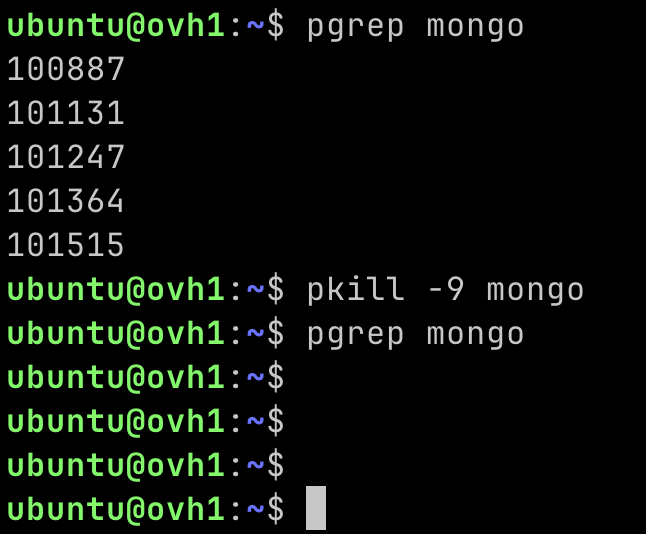
\includegraphics[width=0.3\textwidth]{fotos/mongo/matar_mongo.png}
\caption{Verificación de procesos \textit{mongod} en ejecución}
\label{fig:matar_mongo}
\end{figure}

Rehabilitamos la autenticación, y luego volvemos a lanzar los procesos \texttt{mongod} y \texttt{mongos}. Esta vez no es necesario inicializar los \textit{replicaSets} o agregar los \textit{shards}, ya que el \textit{cluster} mantiene los datos de configuración. Esto lo vemos en la figura \ref{fig:lanzar_mongo}.

\begin{figure}[H]
\centering
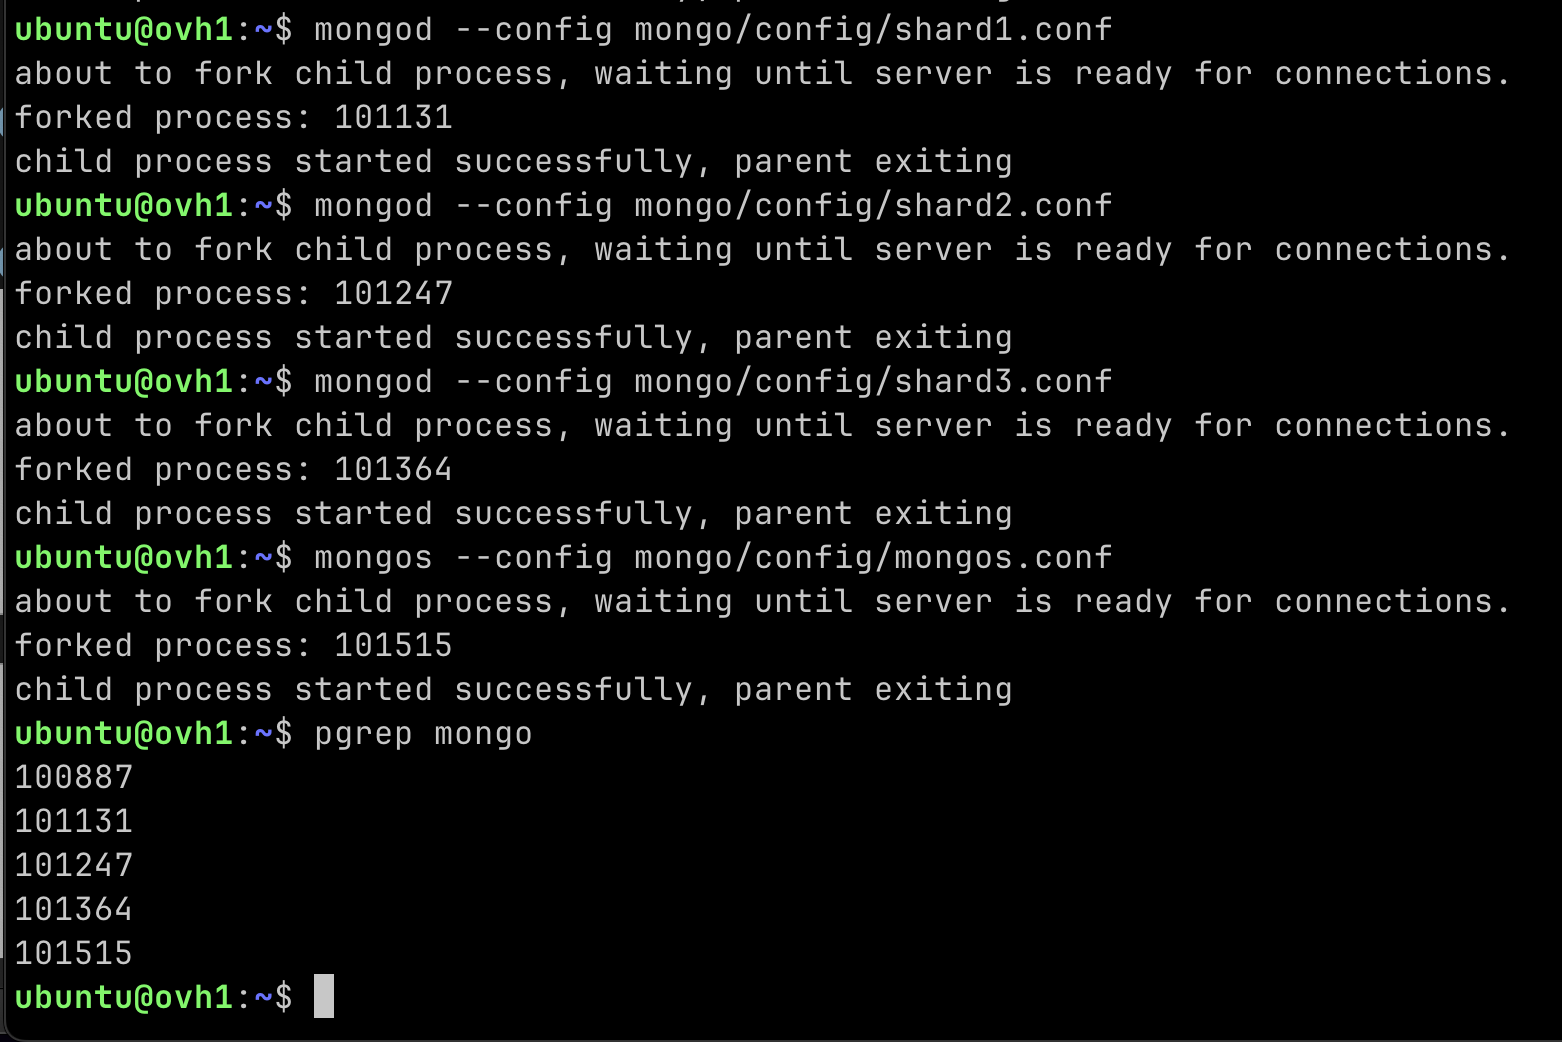
\includegraphics[width=0.6\textwidth]{fotos/mongo/lanzar_mongod.png}
\caption{Lanzamiento de los procesos \textit{mongod} y \textit{mongos}.}
\label{fig:lanzar_mongo}
\end{figure}


\subsection{Extracción de datos para consultas Q1 y Q3}

En la práctica se nos pide diseñar una colección que permita resolver de forma eficiente las consultas Q1 y Q3, consultas centradas en partidos de torneos específicos. Diseñamos, pues, esta colección partiendo de la tabla de partidos, y agregando a cada partido todas las demás tablas, excepto la tabla de \textit{ranking}. \\

En nuestra base de datos relacional, ejecutamos la siguiente instrucción SQL para generar un archivo que contenga los diferentes documentos JSON que importaremos a MongoDB:

\begin{minted}[frame=single, fontsize=\footnotesize]{sql}
COPY (
    SELECT 
        jsonb_build_object(
            'torneo', jsonb_build_object(
                'id', t.id,
                'nombre', t.nombre,
                'fecha', et.fecha,
                'pais', CASE 
                            WHEN tp.codigo_iso2 IS NOT NULL THEN jsonb_build_object(
                                'codigo_iso2', tp.codigo_iso2,
                                'codigo_iso3', tp.codigo_iso3,
                                'codigo_ioc', tp.codigo_ioc,
                                'nombre', tp.nombre
                            )
                            ELSE NULL 
                        END,
                'superficie', et.superficie,
                'tamano', et.tamano,
                'nivel', et.nivel
            ),
            'num_sets', p.num_sets,
            'ronda', p.ronda,
            'desenlace', p.desenlace,
            'ganador', CASE 
                           WHEN jg.id IS NOT NULL THEN jsonb_build_object(
                               'id', jg.id,
                               'nombre', jg.nombre,
                               'apellido', jg.apellido,
                               'diestro', jg.diestro,
                               'fecha_nacimiento', jg.fecha_nacimiento,
                               'altura', jg.altura,
                               'pais', CASE 
                                           WHEN pg.codigo_iso2 IS NOT NULL THEN jsonb_build_object(
                                               'codigo_iso2', pg.codigo_iso2,
                                               'codigo_iso3', pg.codigo_iso3,
                                               'codigo_ioc', pg.codigo_ioc,
                                               'nombre', pg.nombre
                                           )
                                           ELSE NULL 
                                       END,
                               'stats', jsonb_build_object(
                                   'aces', p.num_aces_ganador,
                                   'dobles_faltas', p.num_dob_faltas_ganador,
                                   'puntos_servidos', p.num_ptos_servidos_ganador,
                                   'primeros_servicios', p.num_primeros_servicios_ganador,
                                   'primeros_servicios_ganados', p.num_primeros_servicios_ganados_ganador,
                                   'segundos_servicios_ganados', p.num_segundos_servicios_ganados_ganador,
                                   'juegos_servidos', p.num_juegos_servidos_ganador,
                                   'breaks_salvados', p.num_break_salvados_ganador,
                                   'breaks_afrontados', p.num_break_afrontados_ganador
                               )
                           )
                           ELSE NULL 
                       END,
            'perdedor', CASE 
                            WHEN jp.id IS NOT NULL THEN jsonb_build_object(
                                'id', jp.id,
                                'nombre', jp.nombre,
                                'apellido', jp.apellido,
                                'diestro', jp.diestro,
                                'fecha_nacimiento', jp.fecha_nacimiento,
                                'altura', jp.altura,
                                'pais', CASE 
                                            WHEN pp.codigo_iso2 IS NOT NULL THEN jsonb_build_object(
                                                'codigo_iso2', pp.codigo_iso2,
                                                'codigo_iso3', pp.codigo_iso3,
                                                'codigo_ioc', pp.codigo_ioc,
                                                'nombre', pp.nombre
                                            )
                                            ELSE NULL 
                                        END,
                                'stats', jsonb_build_object(
                                    'aces', p.num_aces_perdedor,
                                    'dobles_faltas', p.num_dob_faltas_perdedor,
                                    'puntos_servidos', p.num_ptos_servidos_perdedor,
                                    'primeros_servicios', p.num_primeros_servicios_perdedor,
                                    'primeros_servicios_ganados', p.num_primeros_servicios_ganados_perdedor,
                                    'segundos_servicios_ganados', p.num_segundos_servicios_ganados_perdedor,
                                    'juegos_servidos', p.num_juegos_servidos_perdedor,
                                    'breaks_salvados', p.num_break_salvados_perdedor,
                                    'breaks_afrontados', p.num_break_afrontados_perdedor
                                )
                            )
                            ELSE NULL 
                        END,
            'sets', (
                SELECT jsonb_agg(
                    jsonb_build_object(
                        'num_set', sp.num_set,
                        'juegos_ganador', sp.juegos_ganador,
                        'juegos_perdedor', sp.juegos_perdedor,
                        'puntos_tiebreak_perdedor', sp.puntos_tiebreak_perdedor
                    )
                )
                FROM sets_partido sp
                WHERE sp.torneo = p.torneo AND sp.fecha = p.fecha AND sp.num_partido = p.num_partido
            )
        )
    FROM 
        partido p
        JOIN edicion_torneo et ON p.torneo = et.torneo AND p.fecha = et.fecha
        JOIN torneo t ON et.torneo = t.id
        LEFT JOIN pais tp ON t.pais = tp.codigo_iso2
        LEFT JOIN jugador jg ON p.ganador = jg.id
        LEFT JOIN pais pg ON jg.pais = pg.codigo_iso2
        LEFT JOIN jugador jp ON p.perdedor = jp.id
        LEFT JOIN pais pp ON jp.pais = pp.codigo_iso2
) TO '/tmp/tenis.json';
\end{minted}

\noindent Al ejecutarla, nos genera el archivo \texttt{tenis.json}, que contiene documentos JSON con el siguiente formato:

\begin{minted}[frame=single, fontsize=\footnotesize]{json}
{
  "sets": [
    {
      "num_set": 1,
      "juegos_ganador": 6,
      "juegos_perdedor": 4,
      "puntos_tiebreak_perdedor": null
    },
    {
      "num_set": 2,
      "juegos_ganador": 5,
      "juegos_perdedor": 7,
      "puntos_tiebreak_perdedor": null
    },
    {
      "num_set": 3,
      "juegos_ganador": 6,
      "juegos_perdedor": 4,
      "puntos_tiebreak_perdedor": null
    }
  ],
  "ronda": "R32",
  "torneo": {
    "id": 112,
    "pais": {
      "nombre": "United Kingdom",
      "codigo_ioc": "GBR",
      "codigo_iso2": "GB",
      "codigo_iso3": "GBR"
    },
    "fecha": "2019-07-07",
    "nivel": "A",
    "nombre": "Newport",
    "tamano": 32,
    "superficie": "Hierba"
  },
  "ganador": {
    "id": 105815,
    "pais": {
      "nombre": "United States of America",
      "codigo_ioc": "USA",
      "codigo_iso2": "US",
      "codigo_iso3": "USA"
    },
    "stats": {
      "aces": 8,
      "dobles_faltas": 4,
      "breaks_salvados": 4,
      "juegos_servidos": 16,
      "puntos_servidos": 113,
      "breaks_afrontados": 6,
      "primeros_servicios": 57,
      "primeros_servicios_ganados": 46,
      "segundos_servicios_ganados": 25
    },
    "altura": 188,
    "nombre": "Tennys",
    "diestro": true,
    "apellido": "Sandgren",
    "fecha_nacimiento": "1991-07-07"
  },
  "num_sets": 3,
  "perdedor": {
    "id": 104797,
    "pais": {
      "nombre": "Uzbekistan",
      "codigo_ioc": "UZB",
      "codigo_iso2": "UZ",
      "codigo_iso3": "UZB"
    },
    "stats": {
      "aces": 1,
      "dobles_faltas": 4,
      "breaks_salvados": 5,
      "juegos_servidos": 16,
      "puntos_servidos": 101,
      "breaks_afrontados": 8,
      "primeros_servicios": 60,
      "primeros_servicios_ganados": 43,
      "segundos_servicios_ganados": 20
    },
    "altura": 188,
    "nombre": "Denis",
    "diestro": true,
    "apellido": "Istomin",
    "fecha_nacimiento": "1986-09-09"
  },
  "desenlace": "N"
}
\end{minted}

\subsection{Indexación, sharding y carga de datos}

A la hora de distribuir los datos, debemos también indexar el atributo que vayamos a utilizar como clave de partición. Elegimos indexar y particionar por el atributo \texttt{torneo.nombre} mediante \textit{hash}, ya que es empleado en casi todas las consultas y presenta una alta cardinalidad. Deberemos comprobar, después de importar los documentos, cuántos \textit{chunks} guarda cada \textit{shard} para verificar que existe un reparto equitativo. Ajustamos el valor del tamaño de \textit{chunks}, por defecto 128 \textit{megabytes} en MongoDB 6.0, a un tamaño de 8 megas, para forzar la distribución de los datos entre todos los \textit{shards}:

\newpage

\begin{minted}[frame=single, fontsize=\footnotesize]{js}
use tenis

db.createCollection('partidos')

db.settings.updateOne(
   { _id: "chunksize" },
   { $set: { _id: "chunksize", value: 8 } },
   { upsert: true }
)

db.partidos.createIndex({"torneo.nombre": "hashed"})
sh.shardCollection("tenis.partidos", {"torneo.nombre":"hashed"})
\end{minted}

\noindent Generamos y cargamos los datos desde ovh1:

\begin{minted}[frame=single, fontsize=\footnotesize]{bash}
psql service=citus -f 4.mongo/sql_to_json.sql
mongoimport --host ovh1 --port 27017 --db tenis2 --collection partidos --file /tmp/tenis.json --authenticationDatabase admin -u admin -p ***
\end{minted}

\noindent Debemos verificar que nuestro \textit{cluster} ha reparticionado los datos de forma equitativa entre todos los nodos. Esto lo vemos en la figura \ref{fig:chunks} y lo hacemos con el siguiente comando:

\begin{minted}[frame=single, fontsize=\footnotesize]{js}
sh.status()
\end{minted}

\begin{figure}[H]
\centering
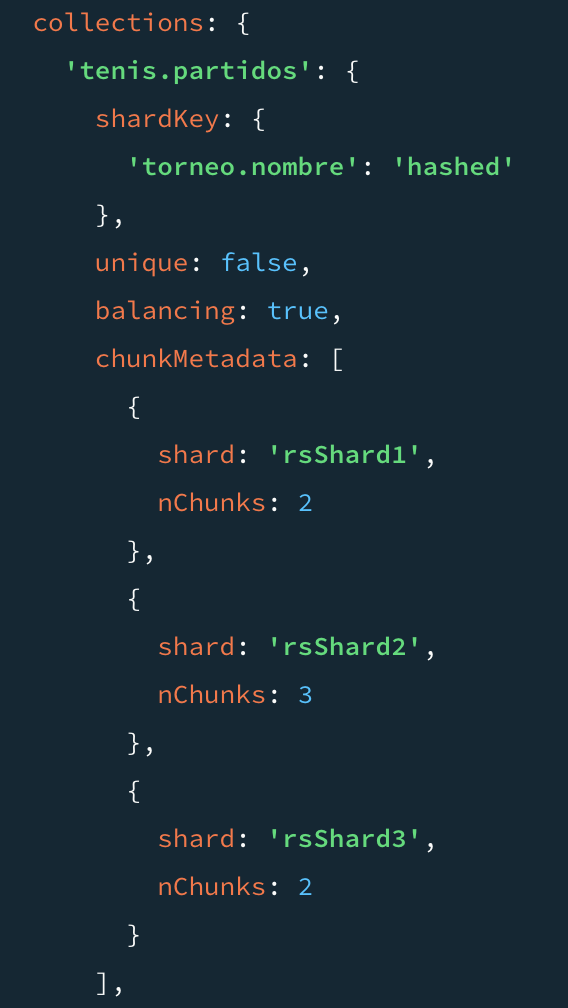
\includegraphics[width=0.3\textwidth]{fotos/mongo/chunks.png}
\caption{Verificación del reparto equitativo de los datos en los nodos del cluster en MongoDB.}
\label{fig:chunks}
\end{figure}




\newpage

\subsection{Consultas MongoDB}

\subsubsection{Muestra todos los ganadores del torneo ``Wimbledon'' (Nombre apellidos y año). Ordena el resultado por año.}

Esta consulta (cuyo resultado vemos en la figura \ref{fig:q1_mongo}) está compuesta por tres etapas en un \texttt{pipeline} de agregación:

\begin{enumerate}
    \item \textbf{\$match:} Filtramos los documentos para incluir solo aquellos del torneo ``Wimbledon'' y de la ronda final (`F').
    \item \textbf{\$project:} Seleccionamos los campos que se mostrarán en el resultado. En este caso:
    \begin{itemize}
        \item Excluye el campo \_id.
        \item Muestra el nombre y apellido del ganador.
        \item Extrae y muestra el año de la fecha del torneo.
    \end{itemize}
    
    \item \textbf{\$sort:} Ordenamos los documentos por el año de forma ascendente.
\end{enumerate}

\begin{minted}[frame=single, fontsize=\footnotesize]{js}
db.partidos.aggregate([
  {
    $match: {
      "torneo.nombre": "Wimbledon",
      ronda: "F",
    },
  },
  {
    $project: {
      _id: 0,
      nombre: "$ganador.nombre",
      apellido: "$ganador.apellido",
      año: {
        $year: {
          $toDate: "$torneo.fecha",
        },
      },
    },
  },
  {
    $sort: {
      año: 1,
    },
  },
]);
\end{minted}

\begin{figure}[H]
\centering
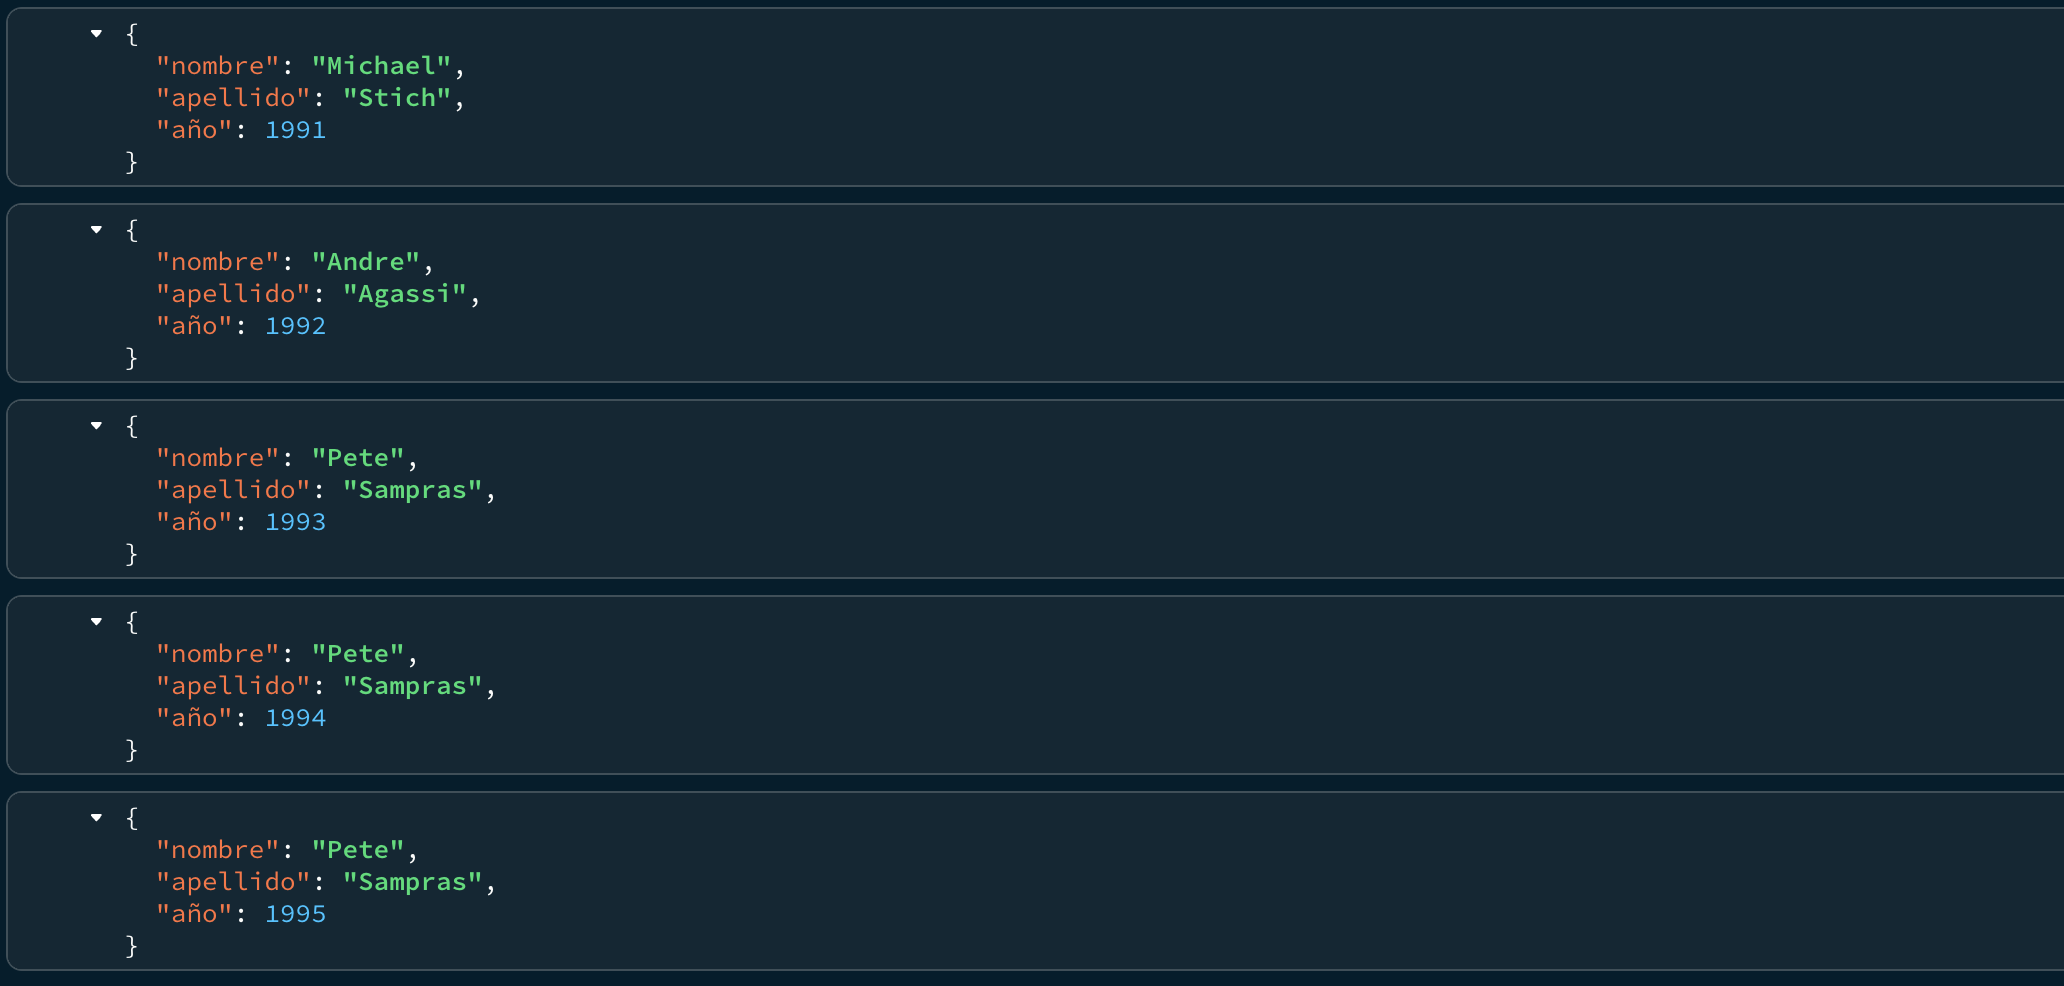
\includegraphics[width=0.6\textwidth]{fotos/mongo/q1.png}
\caption{Bases de datos NoSQL. MongoDB, consulta 1. Al no caber en la propia pantalla, mostramos parte del resultado.}
\label{fig:q1_mongo}
\end{figure}


\subsubsection{Muestra los años en los que Roger Federer ganó algún torneo de nivel Gran Slam (G) o Master 1000 (M). Para cada año, muestra el número de torneos y lista sus nombres (ordenados por la fecha de celebración). Ordena el resultado por el año}

Esta consulta (cuyo resultado mostramos en la figura \ref{fig:q2_mongo}) consta de seis etapas en el \texttt{pipeline} de agregación:

\begin{enumerate}
    \item \textbf{\$match:} Filtramos los documentos para incluir solo aquellos en los que el apellido del ganador es "Federer", el nivel del torneo está en los valores "G" o "M", y la ronda es la final ("F").
    \item \textbf{\$addFields:} Agregamos un nuevo campo \texttt{año}, que contiene el año extraído de la fecha del torneo.
    \item \textbf{\$group:} Agrupamos los documentos por el campo \texttt{año}, contando el total de torneos por año (\texttt{total}), y construimos un \textit{array} de torneos (\texttt{torneos}) con el nombre y la fecha de cada torneo.
    \item \textbf{\$addFields:} Dentro de la etapa de agregar campos, ordenamos el \textit{array} de torneos por la fecha de celebración del torneo de manera ascendente.
    \item \textbf{\$project:} Proyectamos los campos del resultado final. Excluimos el campo \_id, pero mostramos el año y el total de torneos por año. Además, convertimos el \textit{array} de torneos en una cadena de texto separada por comas, listando los nombres de los torneos en orden.
    \item \textbf{\$sort:} Ordenamos los resultados por el campo \texttt{año} de manera ascendente.
\end{enumerate}

\begin{minted}[frame=single, fontsize=\footnotesize]{js}
db.partidos.aggregate([
  {
    $match: {
      "ganador.apellido": "Federer",
      "torneo.nivel": { $in: ["G", "M"] },
      ronda: "F",
    },
  },
  {
    $addFields: {
      año: {
        $year: { $toDate: "$torneo.fecha" },
      },
    },
  },
  {
    $group: {
      _id: "$año",
      total: { $sum: 1 },
      torneos: {
        $push: {
          nombre: "$torneo.nombre",
          fecha: { $toDate: "$torneo.fecha" },
        },
      },
    },
  },
  {
    $addFields: {
      torneos: {
        $sortArray: {
          input: "$torneos",
          sortBy: { fecha: 1 },
        },
      },
    },
  },
  {
    $project: {
      _id: 0,
      año: "$_id",
      total: "$total",

      torneos: {
        $reduce: {
          input: "$torneos.nombre",
          initialValue: "",
          in: {
            $cond: {
              if: { $eq: ["$$value", ""] },
              then: "$$this",
              else: {
                $concat: ["$$value", ", ", "$$this"],
              },
            },
          },
        },
      },
    },
  },
  {
    $sort: { año: 1 },
  },
]);
\end{minted}

\begin{figure}[H]
\centering
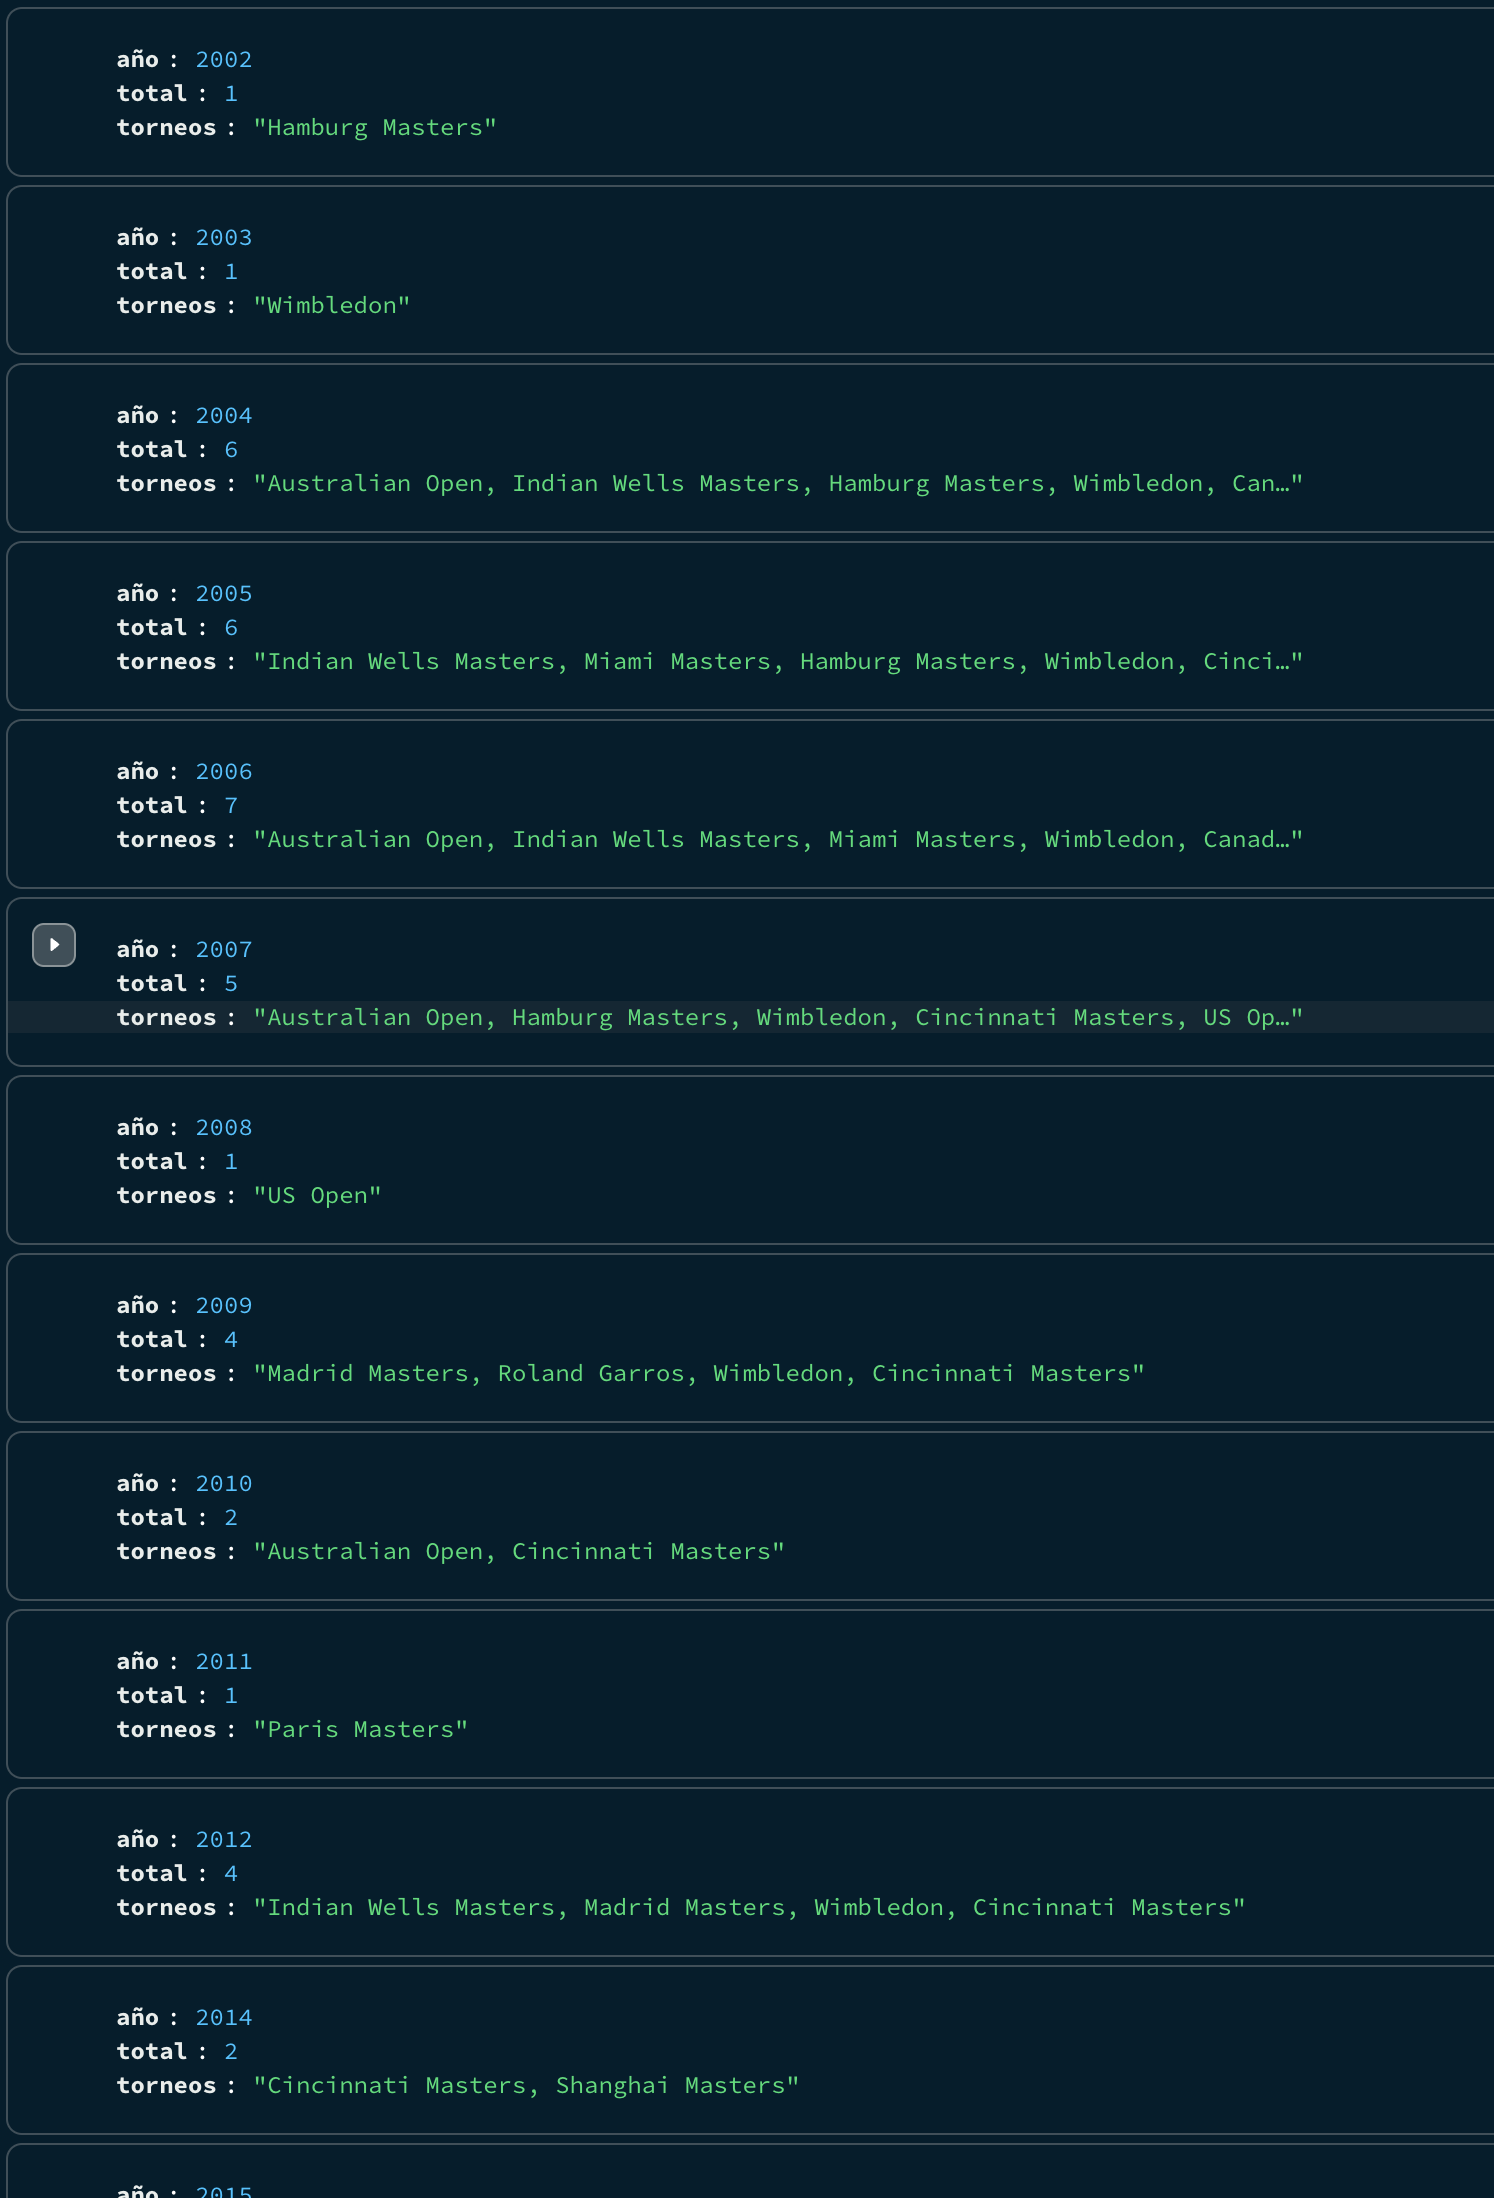
\includegraphics[width=0.45\textwidth]{fotos/mongo/q2.png}
\caption{Bases de datos NoSQL. MongoDB, consulta 2.}
\label{fig:q2_mongo}
\end{figure}


\subsubsection{Muestra los partidos de semifinales (ronda='SF') y final (ronda = 'F') del torneo de "Roland Garros" del 2018. Para cada partido muestra la ronda, el tipo de desenlace, el nombre y apellidos del ganador y el nombre y apellidos del perdedor y el resultado con el número de juegos del ganador y del perdedor en cada set, y opcionalmente en paréntesis el número de juegos del perdedor en el tie break}

Esta consulta (cuyo resultado vemos en la figura \ref{fig:q3_mongo}) consta de tres etapas en el \texttt{pipeline} de agregación:

\begin{enumerate}
    \item \textbf{\$match:} Filtramos los documentos para obtener los partidos del torneo \texttt{"Roland Garros"} que se jugaron en el año 2018. Además, seleccionamos solo los partidos que se juegan en las rondas \texttt{SF} (semifinal) o \texttt{F} (final).
    \item \textbf{\$addFields:} Agregamos un campo nuevo llamado \texttt{resultado} que concatena los resultados de los sets del partido en el siguiente formato: \texttt{juegos\_ganador-juegos\_perdedor}. Si el set contiene puntos de \textit{tiebreak} para el perdedor, los incluimos entre paréntesis después del marcador, y si no hay \textit{tiebreak}, se omite. Este campo contiene la cadena de resultados de todos los sets jugados en el partido.
    \item \textbf{\$project:} Proyectamos los campos seleccionados en el resultado final. Excluyimos el campo \_id, y muestramos la \texttt{ronda}, el \texttt{desenlace}, el nombre completo del \texttt{ganador} (concatenando el \texttt{nombre} y \texttt{apellido}), el nombre completo del \texttt{perdedor} (concatenando \texttt{nombre} y \texttt{apellido}), y el campo \texttt{resultado} que fue generado en la etapa anterior.
\end{enumerate}

\begin{minted}[frame=single, fontsize=\footnotesize]{js}
db.partidos.aggregate([
  {
    $match: {
      "torneo.nombre": "Roland Garros",
      $expr: {
        $eq: [{ $year: { $toDate: "$torneo.fecha" } }, 2018],
      },
      ronda: { $in: ["SF", "F"] },
    },
  },
  {
    $addFields: {
      resultado: {
        $reduce: {
          input: "$sets",
          initialValue: "",
          in: {
            $concat: [
              "$$value",
              {
                $cond: {
                  if: { $eq: ["$$value", ""] },
                  then: "",
                  else: " ",
                },
              },
              {
                $toString: "$$this.juegos_ganador",
              },
              "-",
              {
                $toString: "$$this.juegos_perdedor",
              },
              {
                $cond: {
                  if: {
                    $ne: ["$$this.puntos_tiebreak_perdedor", null],
                  },
                  then: {
                    $concat: [
                      "(",
                      {
                        $toString: "$$this.puntos_tiebreak_perdedor",
                      },
                      ")",
                    ],
                  },
                  else: "",
                },
              },
            ],
          },
        },
      },
    },
  },
  {
    $project: {
      _id: 0,
      ronda: 1,
      desenlace: 1,
      ganador: {
        $concat: ["$ganador.nombre", " ", "$ganador.apellido"],
      },
      perdedor: {
        $concat: ["$perdedor.nombre", " ", "$perdedor.apellido"],
      },
      resultado: 1,
    },
  },
]);
\end{minted}

\begin{figure}[H]
\centering
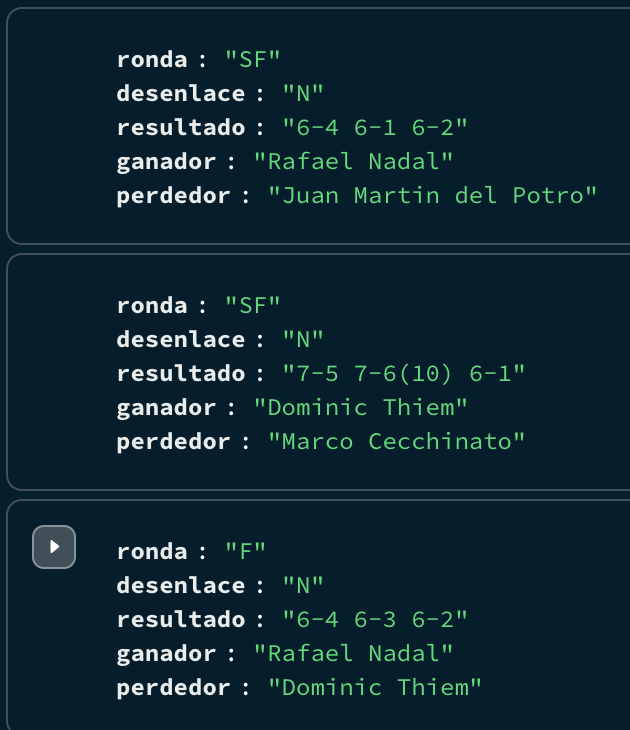
\includegraphics[width=0.4\textwidth]{fotos/mongo/q3.png}
\caption{Bases de datos NoSQL. MongoDB, consulta 3.}
\label{fig:q3_mongo}
\end{figure}


\subsubsection{Muestra la lista de jugadores españoles (ES) que ganaron algún torneo de nivel Gran Slam (G). Para cada jugador muestra los siguientes datos resumen de todos sus partidos: número de partidos jugados, porcentaje de victorias, porcentaje de aces, porcentaje de dobles faltas, porcentaje de servicios ganados, porcentaje de restos ganados, porcentaje de break points salvados (de los sufridos en contra), porcentaje de break points ganados (de los provocados a favor)}

Esta consulta (cuyo resultado mostramos en la figura \ref{fig:q4_mongo} consta de varias etapas en el \texttt{pipeline} de agregación:

\begin{enumerate}
    \item \textbf{\$match:} Filtramos los partidos donde el torneo es de nivel "G" (Grand Slam), la ronda es "F" (final), y el ganador es de España (\texttt{codigo\_iso2} = "ES").
    \item \textbf{\$group:} Agrupamos los documentos por el \texttt{id} del ganador, y para cada grupo obtenemos el nombre completo del jugador (concatenando el \texttt{nombre} y el \texttt{apellido} del ganador) utilizando \texttt{\$first}.
    \item \textbf{\$lookup:} Realizamos una operación de \texttt{join} con la colección \texttt{partidos}, buscando todos los partidos en los que el jugador (basado en su \texttt{id}) haya sido ganador o perdedor. Los resultados los almacenamos en un \textit{array} llamado \texttt{all\_matches}.
    \item \textbf{\$project:} Proyectamos varios campos:
    \begin{itemize}
        \item \texttt{jugador:} El nombre completo del ganador.
        \item \texttt{partidos:} El número de partidos en los que el jugador ha participado, calculado con \texttt{\$size}.
        \item \texttt{pcje\_victorias:} El porcentaje de victorias calculado como la proporción de victorias del jugador sobre el total de partidos jugados, multiplicado por 100.
        \item \texttt{pcje\_aces:} El porcentaje de \textit{aces} ganados, calculado como el total de \textit{aces} en los partidos ganados dividido por el total de puntos servidos.
        \item \texttt{pcje\_dobles\_faltas:} El porcentaje de dobles faltas cometidas, calculado de manera similar a \texttt{pcje\_aces}.
        \item \texttt{pcje\_servicios\_ganados:} El porcentaje de puntos de servicio ganados, basado en los primeros y segundos servicios, calculado por la misma lógica.
        \item \texttt{pcje\_restos\_ganados:} El porcentaje de puntos ganados en los restos de servicio, calculado de manera similar a \texttt{pcje\_servicios\_ganados}.
        \item \texttt{pcje\_breaks\_salvados:} El porcentaje de \textit{breaks} salvados en comparación con los \textit{breaks} enfrentados, calculado con la misma lógica.
        \item \texttt{pcje\_breaks\_ganados:} El porcentaje de \textit{breaks} ganados comparado con los \textit{breaks} enfrentados.
    \end{itemize}
    \item \textbf{\$project (redondeo):} Redondeamos todos los porcentajes calculados en la etapa anterior a un decimal.
\end{enumerate}

\begin{minted}[frame=single, fontsize=\footnotesize]{js}
db.partidos.aggregate([
  {
    $match: {
      "torneo.nivel": "G",
      ronda: "F",
      "ganador.pais.codigo_iso2": "ES",
    },
  },

  {
    $group: {
      _id: "$ganador.id",
      jugador: {
        $first: {
          $concat: ["$ganador.nombre", " ", "$ganador.apellido"],
        },
      },
    },
  },

  {
    $lookup: {
      from: "partidos",
      let: { playerId: "$_id" },
      pipeline: [
        {
          $match: {
            $expr: {
              $or: [
                {
                  $eq: ["$ganador.id", "$$playerId"],
                },
                {
                  $eq: ["$perdedor.id", "$$playerId"],
                },
              ],
            },
          },
        },
      ],
      as: "all_matches",
    },
  },

  {
    $project: {
      _id: 0,
      jugador: 1,
      partidos: { $size: "$all_matches" },
      pcje_victorias: {
        $multiply: [
          {
            $divide: [
              {
                $size: {
                  $filter: {
                    input: "$all_matches",
                    cond: {
                      $eq: ["$$this.ganador.id", "$_id"],
                    },
                  },
                },
              },
              { $size: "$all_matches" },
            ],
          },
          100,
        ],
      },
      pcje_aces: {
        $multiply: [
          {
            $divide: [
              {
                $sum: {
                  $map: {
                    input: "$all_matches",
                    as: "match",
                    in: {
                      $cond: [
                        {
                          $eq: ["$$match.ganador.id", "$_id"],
                        },
                        "$$match.ganador.stats.aces",
                        "$$match.perdedor.stats.aces",
                      ],
                    },
                  },
                },
              },
              {
                $sum: {
                  $map: {
                    input: "$all_matches",
                    as: "match",
                    in: {
                      $cond: [
                        {
                          $eq: ["$$match.ganador.id", "$_id"],
                        },
                        "$$match.ganador.stats.puntos_servidos",
                        "$$match.perdedor.stats.puntos_servidos",
                      ],
                    },
                  },
                },
              },
            ],
          },
          100,
        ],
      },
      pcje_dobles_faltas: {
        $multiply: [
          {
            $divide: [
              {
                $sum: {
                  $map: {
                    input: "$all_matches",
                    as: "match",
                    in: {
                      $cond: [
                        {
                          $eq: ["$$match.ganador.id", "$_id"],
                        },
                        "$$match.ganador.stats.dobles_faltas",
                        "$$match.perdedor.stats.dobles_faltas",
                      ],
                    },
                  },
                },
              },
              {
                $sum: {
                  $map: {
                    input: "$all_matches",
                    as: "match",
                    in: {
                      $cond: [
                        {
                          $eq: ["$$match.ganador.id", "$_id"],
                        },
                        "$$match.ganador.stats.puntos_servidos",
                        "$$match.perdedor.stats.puntos_servidos",
                      ],
                    },
                  },
                },
              },
            ],
          },
          100,
        ],
      },
      pcje_servicios_ganados: {
        $multiply: [
          {
            $divide: [
              {
                $sum: {
                  $map: {
                    input: "$all_matches",
                    as: "match",
                    in: {
                      $cond: [
                        {
                          $eq: ["$$match.ganador.id", "$_id"],
                        },
                        {
                          $add: [
                            "$$match.ganador.stats.primeros_servicios_ganados",
                            "$$match.ganador.stats.segundos_servicios_ganados",
                          ],
                        },
                        {
                          $add: [
                            "$$match.perdedor.stats.primeros_servicios_ganados",
                            "$$match.perdedor.stats.segundos_servicios_ganados",
                          ],
                        },
                      ],
                    },
                  },
                },
              },
              {
                $sum: {
                  $map: {
                    input: "$all_matches",
                    as: "match",
                    in: {
                      $cond: [
                        {
                          $eq: ["$$match.ganador.id", "$_id"],
                        },
                        "$$match.ganador.stats.puntos_servidos",
                        "$$match.perdedor.stats.puntos_servidos",
                      ],
                    },
                  },
                },
              },
            ],
          },
          100,
        ],
      },
      pcje_restos_ganados: {
        $multiply: [
          {
            $divide: [
              {
                $sum: {
                  $map: {
                    input: "$all_matches",
                    as: "match",
                    in: {
                      $cond: [
                        {
                          $eq: ["$$match.ganador.id", "$_id"],
                        },
                        {
                          $subtract: [
                            "$$match.perdedor.stats.puntos_servidos",
                            {
                              $add: [
                                "$$match.perdedor.stats.primeros_servicios_ganados",
                                "$$match.perdedor.stats.segundos_servicios_ganados",
                              ],
                            },
                          ],
                        },
                        {
                          $subtract: [
                            "$$match.ganador.stats.puntos_servidos",
                            {
                              $add: [
                                "$$match.ganador.stats.primeros_servicios_ganados",
                                "$$match.ganador.stats.segundos_servicios_ganados",
                              ],
                            },
                          ],
                        },
                      ],
                    },
                  },
                },
              },
              {
                $sum: {
                  $map: {
                    input: "$all_matches",
                    as: "match",
                    in: {
                      $cond: [
                        {
                          $eq: ["$$match.ganador.id", "$_id"],
                        },
                        "$$match.perdedor.stats.puntos_servidos",
                        "$$match.ganador.stats.puntos_servidos",
                      ],
                    },
                  },
                },
              },
            ],
          },
          100,
        ],
      },
      pcje_breaks_salvados: {
        $multiply: [
          {
            $divide: [
              {
                $sum: {
                  $map: {
                    input: "$all_matches",
                    as: "match",
                    in: {
                      $cond: [
                        {
                          $eq: ["$$match.ganador.id", "$_id"],
                        },
                        "$$match.ganador.stats.breaks_salvados",
                        "$$match.perdedor.stats.breaks_salvados",
                      ],
                    },
                  },
                },
              },
              {
                $sum: {
                  $map: {
                    input: "$all_matches",
                    as: "match",
                    in: {
                      $cond: [
                        {
                          $eq: ["$$match.ganador.id", "$_id"],
                        },
                        "$$match.ganador.stats.breaks_afrontados",
                        "$$match.perdedor.stats.breaks_afrontados",
                      ],
                    },
                  },
                },
              },
            ],
          },
          100,
        ],
      },
      pcje_breaks_ganados: {
        $multiply: [
          {
            $divide: [
              {
                $sum: {
                  $map: {
                    input: "$all_matches",
                    as: "match",
                    in: {
                      $cond: [
                        {
                          $eq: ["$$match.ganador.id", "$_id"],
                        },
                        {
                          $subtract: [
                            "$$match.perdedor.stats.breaks_afrontados",
                            "$$match.perdedor.stats.breaks_salvados",
                          ],
                        },
                        {
                          $subtract: [
                            "$$match.ganador.stats.breaks_afrontados",
                            "$$match.ganador.stats.breaks_salvados",
                          ],
                        },
                      ],
                    },
                  },
                },
              },
              {
                $sum: {
                  $map: {
                    input: "$all_matches",
                    as: "match",
                    in: {
                      $cond: [
                        {
                          $eq: ["$$match.ganador.id", "$_id"],
                        },
                        "$$match.perdedor.stats.breaks_afrontados",
                        "$$match.ganador.stats.breaks_afrontados",
                      ],
                    },
                  },
                },
              },
            ],
          },
          100,
        ],
      },
    },
  },

  // Round all percentages to 1 decimal place
  {
    $project: {
      jugador: 1,
      partidos: 1,
      pcje_victorias: {
        $round: ["$pcje_victorias", 1],
      },
      pcje_aces: { $round: ["$pcje_aces", 1] },
      pcje_dobles_faltas: {
        $round: ["$pcje_dobles_faltas", 1],
      },
      pcje_servicios_ganados: {
        $round: ["$pcje_servicios_ganados", 1],
      },
      pcje_restos_ganados: {
        $round: ["$pcje_restos_ganados", 1],
      },
      pcje_breaks_salvados: {
        $round: ["$pcje_breaks_salvados", 1],
      },
      pcje_breaks_ganados: {
        $round: ["$pcje_breaks_ganados", 1],
      },
    },
  },
]);
\end{minted}

\begin{figure}[H]
\centering
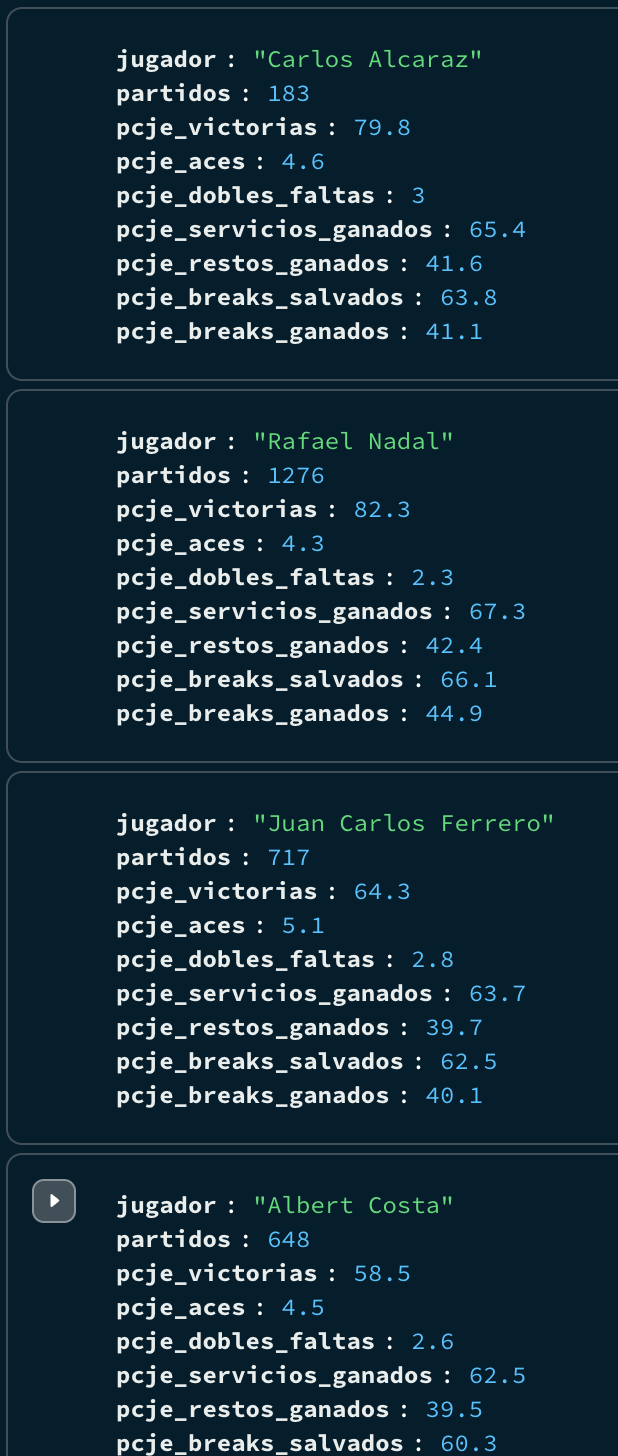
\includegraphics[width=0.3\textwidth]{fotos/mongo/q4.png}
\caption{Bases de datos NoSql. MongoDB, consulta 4. Resultado parcial debido al tamaño del mismo.}
\label{fig:q4_mongo}
\end{figure}




\subsubsection{Lista los jugadores que fueron derrotados (en algún partido del 2018) por el rival de Rafael Nadal de la primera ronda (R128) de Roland Garros de 2018}

Esta consulta (cuyo resultado mostramos en la figura \ref{fig:q5_mongo}) consta de varias etapas en el \texttt{pipeline} de agregación:

\begin{enumerate}
    \item \textbf{\$match:} Filtramos los partidos del torneo \texttt{"Roland Garros"} en el año 2018, específicamente de la ronda \texttt{R128}, y donde al menos uno de los jugadores es \texttt{Rafael Nadal}, ya sea como ganador o perdedor.
    \item \textbf{\$project:} Agregamos un campo \texttt{rival\_id} que determina el \texttt{id} del rival del jugador \texttt{Rafael Nadal}. Si \texttt{Rafael Nadal} es el ganador del partido, se asigna el \texttt{id} del perdedor; de lo contrario, se asigna el \texttt{id} del ganador.
    
    \item \textbf{\$lookup:} Realizamos una operación de \texttt{join} con la colección \texttt{partidos}, buscando los partidos donde el \texttt{id} del rival aparece como ganador. El resultado de esta operación se almacena en el campo \texttt{partidos\_rival}.
    
    \item \textbf{\$unwind:} Descomponemos el \textit{array} \texttt{partidos\_rival} para obtener un único documento por cada partido encontrado. Esto convierte los elementos del \textit{array} en documentos separados dentro del flujo.
    \item \textbf{\$match:} Filtramos los documentos para asegurarse de que los partidos de la colección \texttt{partidos\_rival} sean del año 2018, usando el operador \texttt{\$year} en la fecha del torneo.
    \item \textbf{\$project:} Proyectamos el nombre y apellido del \texttt{perdedor} de cada partido del rival, concatenando ambos en un solo campo \texttt{jugador}. También proyectamos el código de país (\texttt{codigo\_iso2}) del \texttt{perdedor} del partido del rival.
\end{enumerate}

\begin{minted}[frame=single, fontsize=\footnotesize]{js}
db.partidos.aggregate([
  {
    $match: {
      "torneo.nombre": "Roland Garros",
      $expr: {
        $eq: [{ $year: { $toDate: "$torneo.fecha" } }, 2018],
      },
      ronda: "R128",
      $or: [
        {
          "ganador.nombre": "Rafael",
          "ganador.apellido": "Nadal",
        },
        {
          "perdedor.nombre": "Rafael",
          "perdedor.apellido": "Nadal",
        },
      ],
    },
  },

  {
    $project: {
      rival_id: {
        $cond: [
          {
            $and: [
              {
                $eq: ["$ganador.nombre", "Rafael"],
              },
              {
                $eq: ["$ganador.apellido", "Nadal"],
              },
            ],
          },
          "$perdedor.id",
          "$ganador.id",
        ],
      },
    },
  },

  {
    $lookup: {
      from: "partidos",
      localField: "rival_id",
      foreignField: "ganador.id",
      as: "partidos_rival",
    },
  },
  {
    $unwind: "$partidos_rival",
  },
  {
    $match: {
      $expr: {
        $eq: [
          {
            $year: {
              $toDate: "$partidos_rival.torneo.fecha",
            },
          },
          2018,
        ],
      },
    },
  },
  {
    $project: {
      _id: 0,
      jugador: {
        $concat: [
          "$partidos_rival.perdedor.nombre",
          " ",
          "$partidos_rival.perdedor.apellido",
        ],
      },
      pais: "$partidos_rival.perdedor.pais.codigo_iso2",
    },
  },
]);
\end{minted}

\begin{figure}[H]
\centering
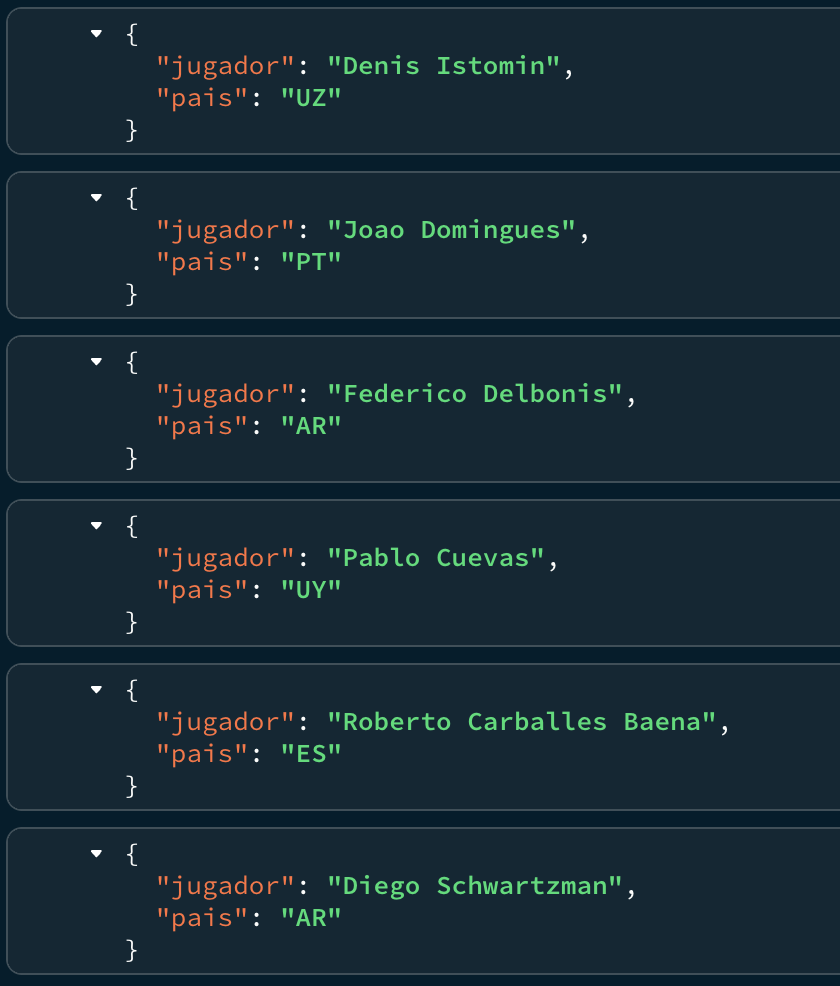
\includegraphics[width=0.38\textwidth]{fotos/mongo/q5.png}
\caption{Bases de datos NoSQL. MongoDB, consulta 5.}
\label{fig:q5_mongo}
\end{figure}



\subsection{Preferencias y compromiso de lectura}

Procedemos ahora a comprobar si el \textit{cluster} sigue funcionando al retirar nodos. Para probar esto, creamos una consulta de prueba que fuerce a MongoDB a emplear datos de todos los \textit{shards}. La consulta que planteamos agrega el total de partidos con desenlace normal:

\begin{minted}[frame=single, fontsize=\footnotesize]{js}
db.partidos.aggregate([  
    {$match: { desenlace: "N" } },
    {$count: "partidos_con_desenlace_normal"},
]);
\end{minted}

Procedemos a parar todos los procesos de MongoDB en un nodo como ya hemos visto anteriormente, y comprobamos que la consulta sigue ejecutándose correctamente. Al dejar un solo nodo activo, la consulta ya no puede ejecutarse y nos devuelve un error (ver figura \ref{fig:error_mongoD}).

\begin{figure}[H]
\centering
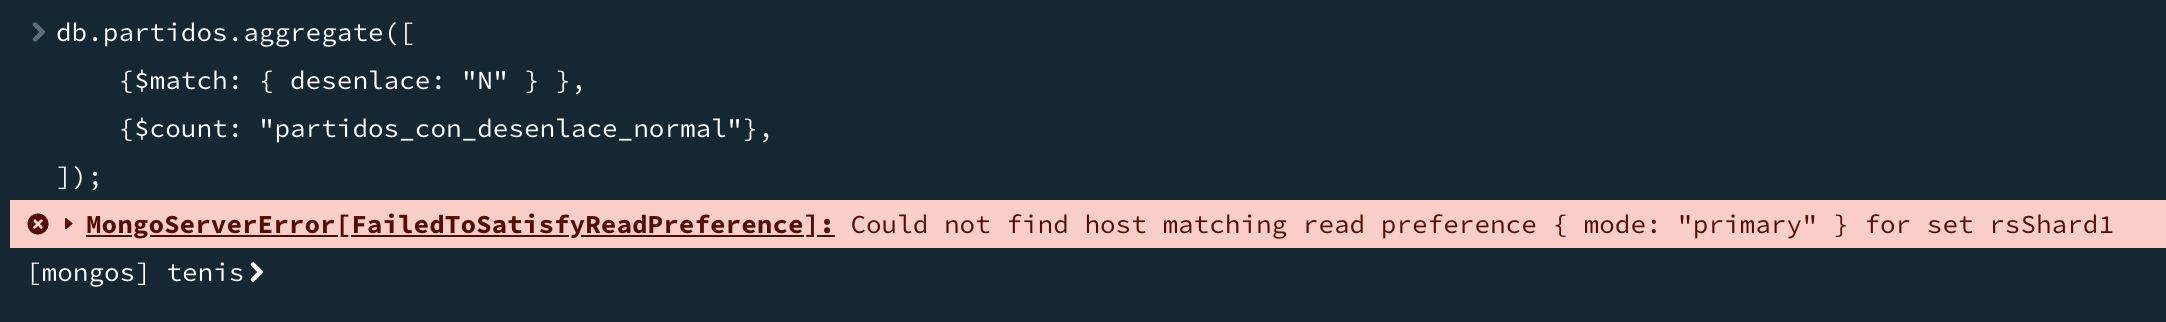
\includegraphics[width=0.9\textwidth]{fotos/mongo/1_node_Error.png}
\caption{Error en MongoDB al retirar nodos.}
\label{fig:error_mongoD}
\end{figure}

Comprobamos cuál es la preferencia de lectura, que por defecto está configurada para leer desde el primario, y el compromiso de lectura, por defecto, lectura local sin garantía de leer los datos más recientes (figura \ref{fig:comprobarpermisos}.

\begin{figure}[H]
     \centering
     \begin{subfigure}[b]{0.45\textwidth}
        \centering
        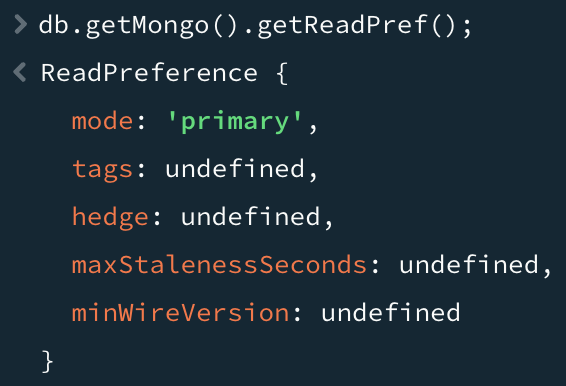
\includegraphics[width=\textwidth]{fotos/mongo/read_pref_default.png}
        \caption{Preferencias de lectura en nuestro \textit{cluster}.}
     \end{subfigure}
     \hfill
     \begin{subfigure}[b]{0.45\textwidth}
        \centering
        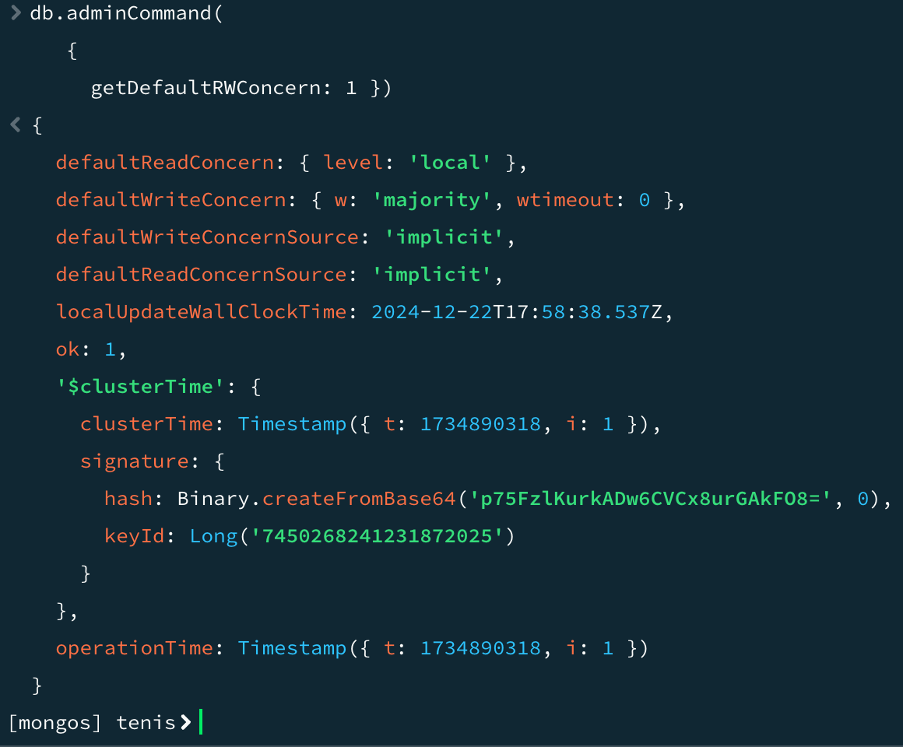
\includegraphics[width=\textwidth]{fotos/mongo/Picture 1.png}
        \caption{Compromiso de lectura en nuestro \textit{cluster}.}
     \end{subfigure}
\caption{Verificación de nodos del \textit{cluster}.}
\label{fig:comprobarpermisos}
\end{figure}

Podemos concluir que uno de los nodos eliminados era el primario, y que el nodo que queda vivo es un secundario que no ha sido capaz de promocionarse a primario, ya que no quedan nodos vivos con los cuales comunicarse para establecer una votación. \\

Si cambiamos las preferencias de lectura a cualquiera que no obligue a leer del primario, las consultas volverán a funcionar (figura \ref{fig:mongo_prueba}).

\begin{figure}[H]
\centering
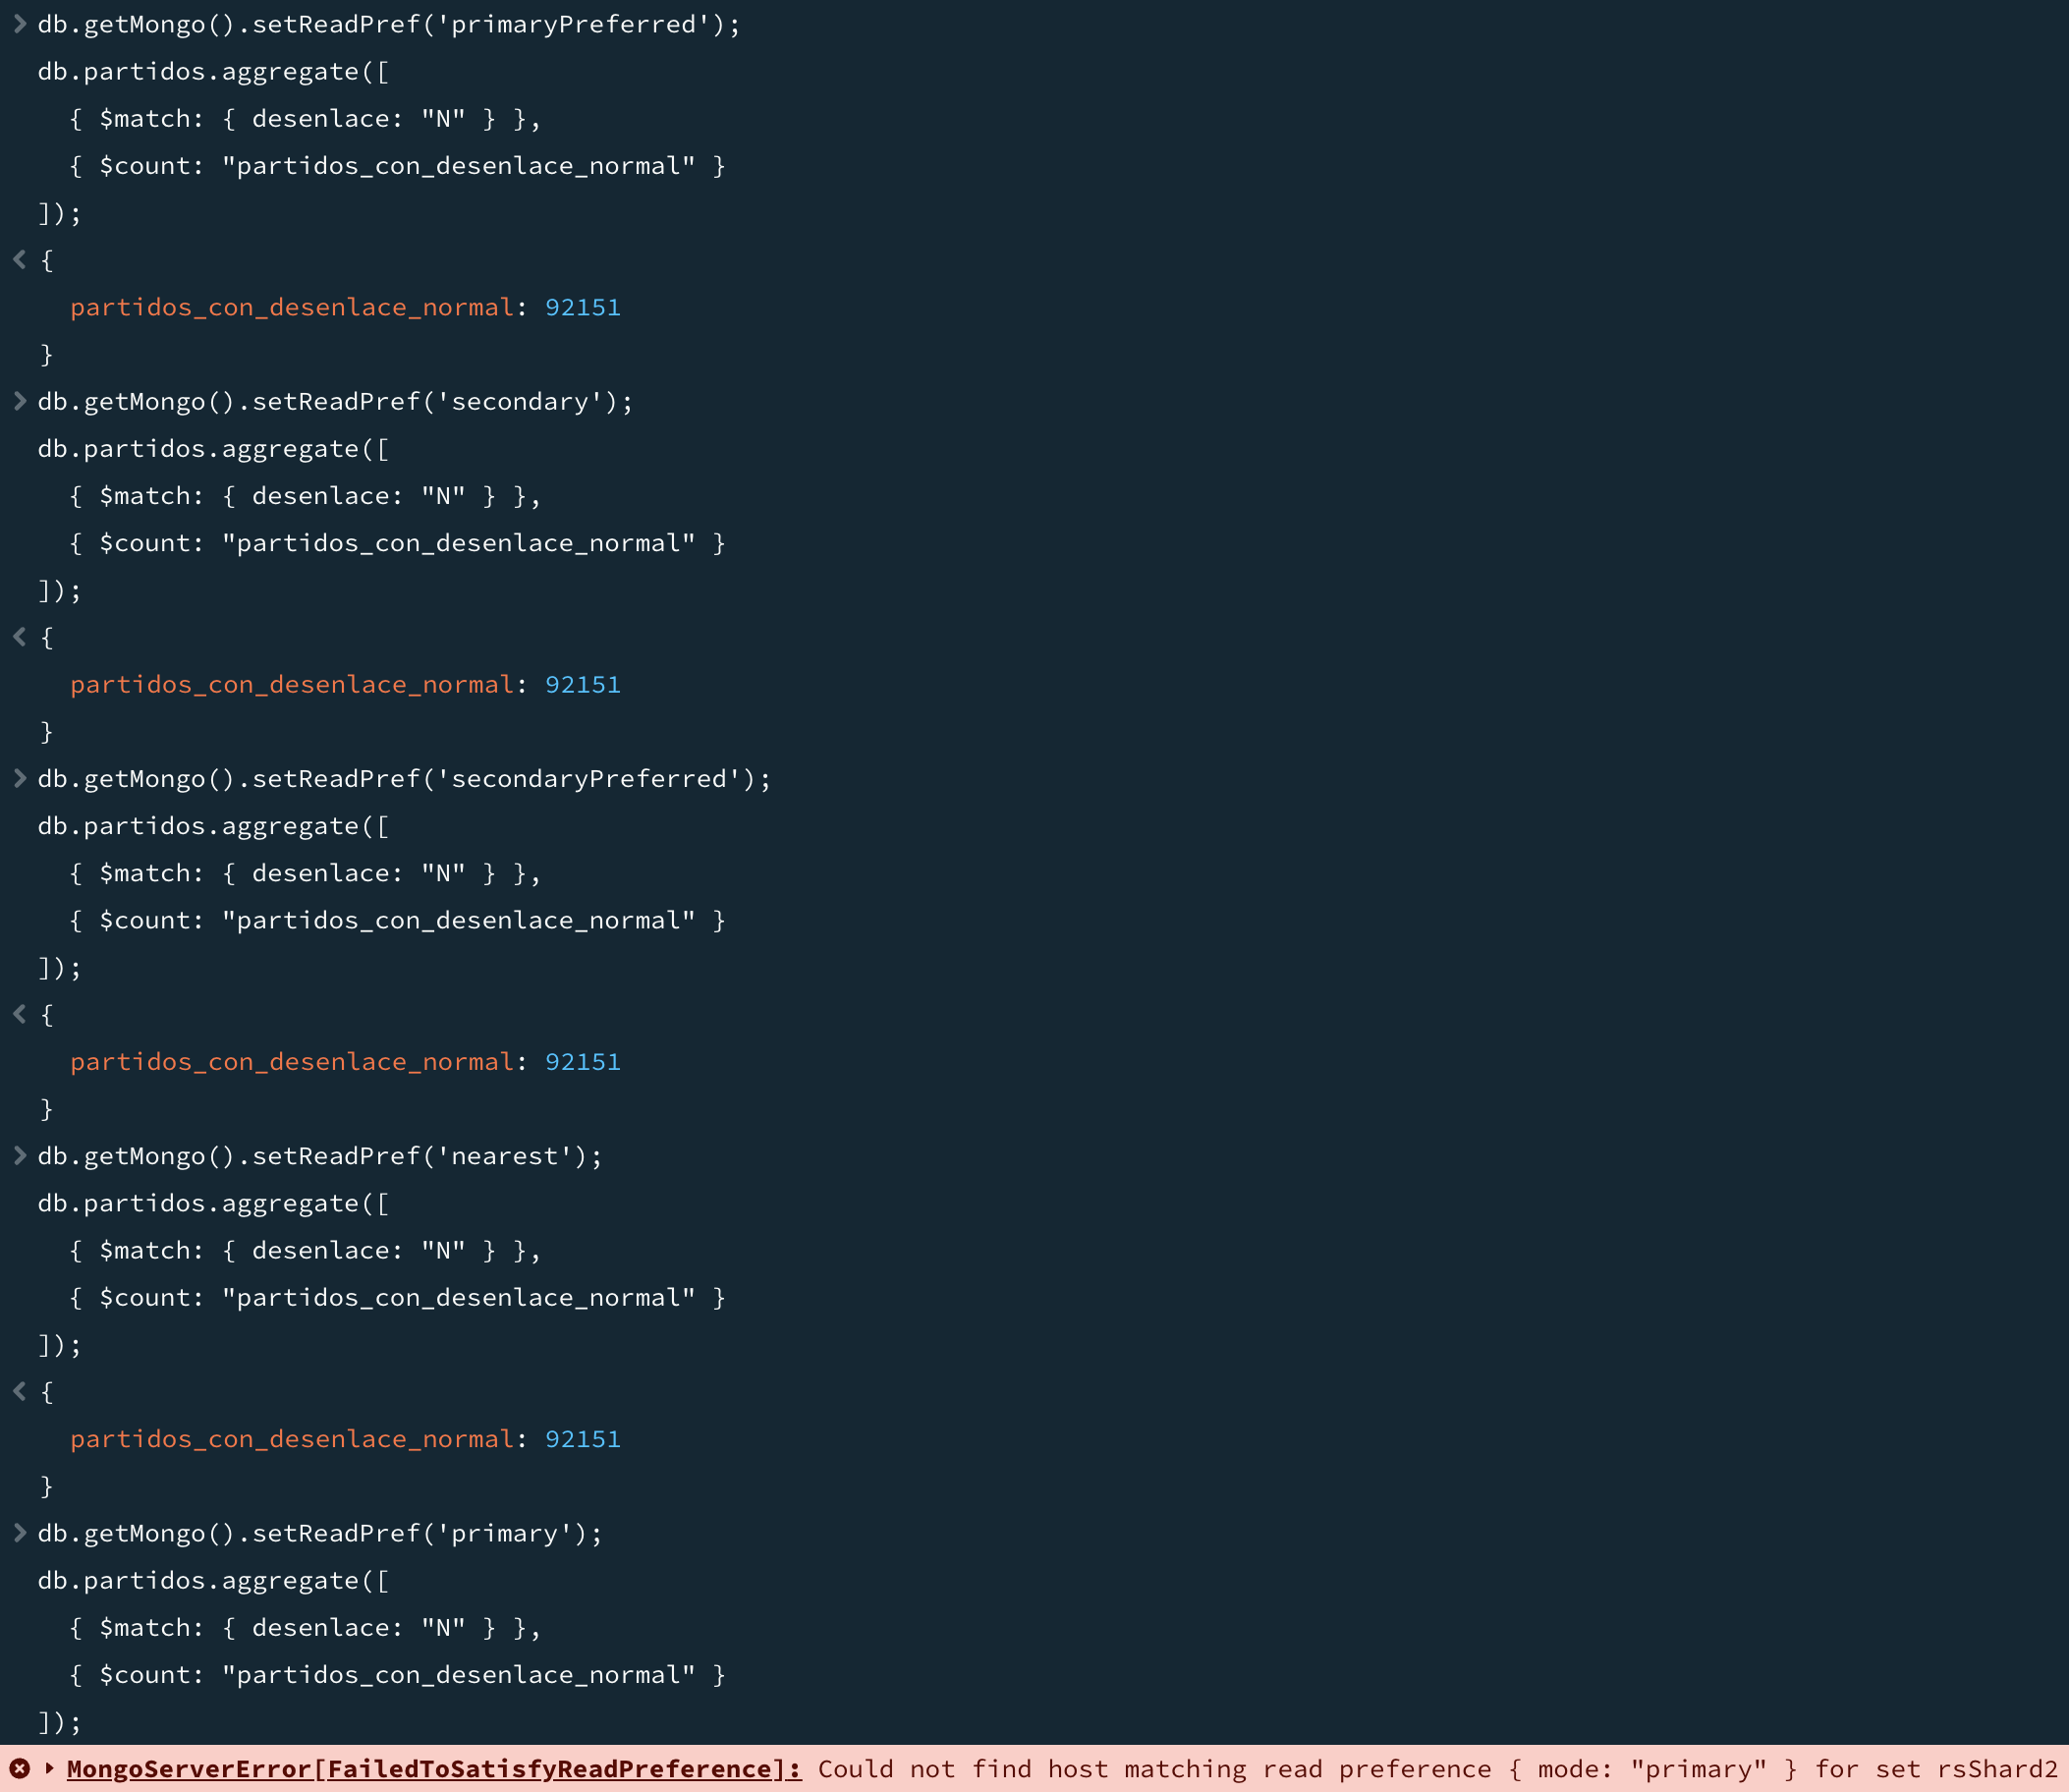
\includegraphics[width=0.7\textwidth]{fotos/mongo/readPRefsResults.png}
\caption{Resultados de consulta de prueba.}
\label{fig:mongo_prueba}
\end{figure}

Fijando la preferencia de lectura en \textbf{primaryPreferred}, procedemos ahora a ver cómo afecta el compromiso de lectura a la posibilidad de ejecutar la consulta.

\begin{figure}[H]
\centering
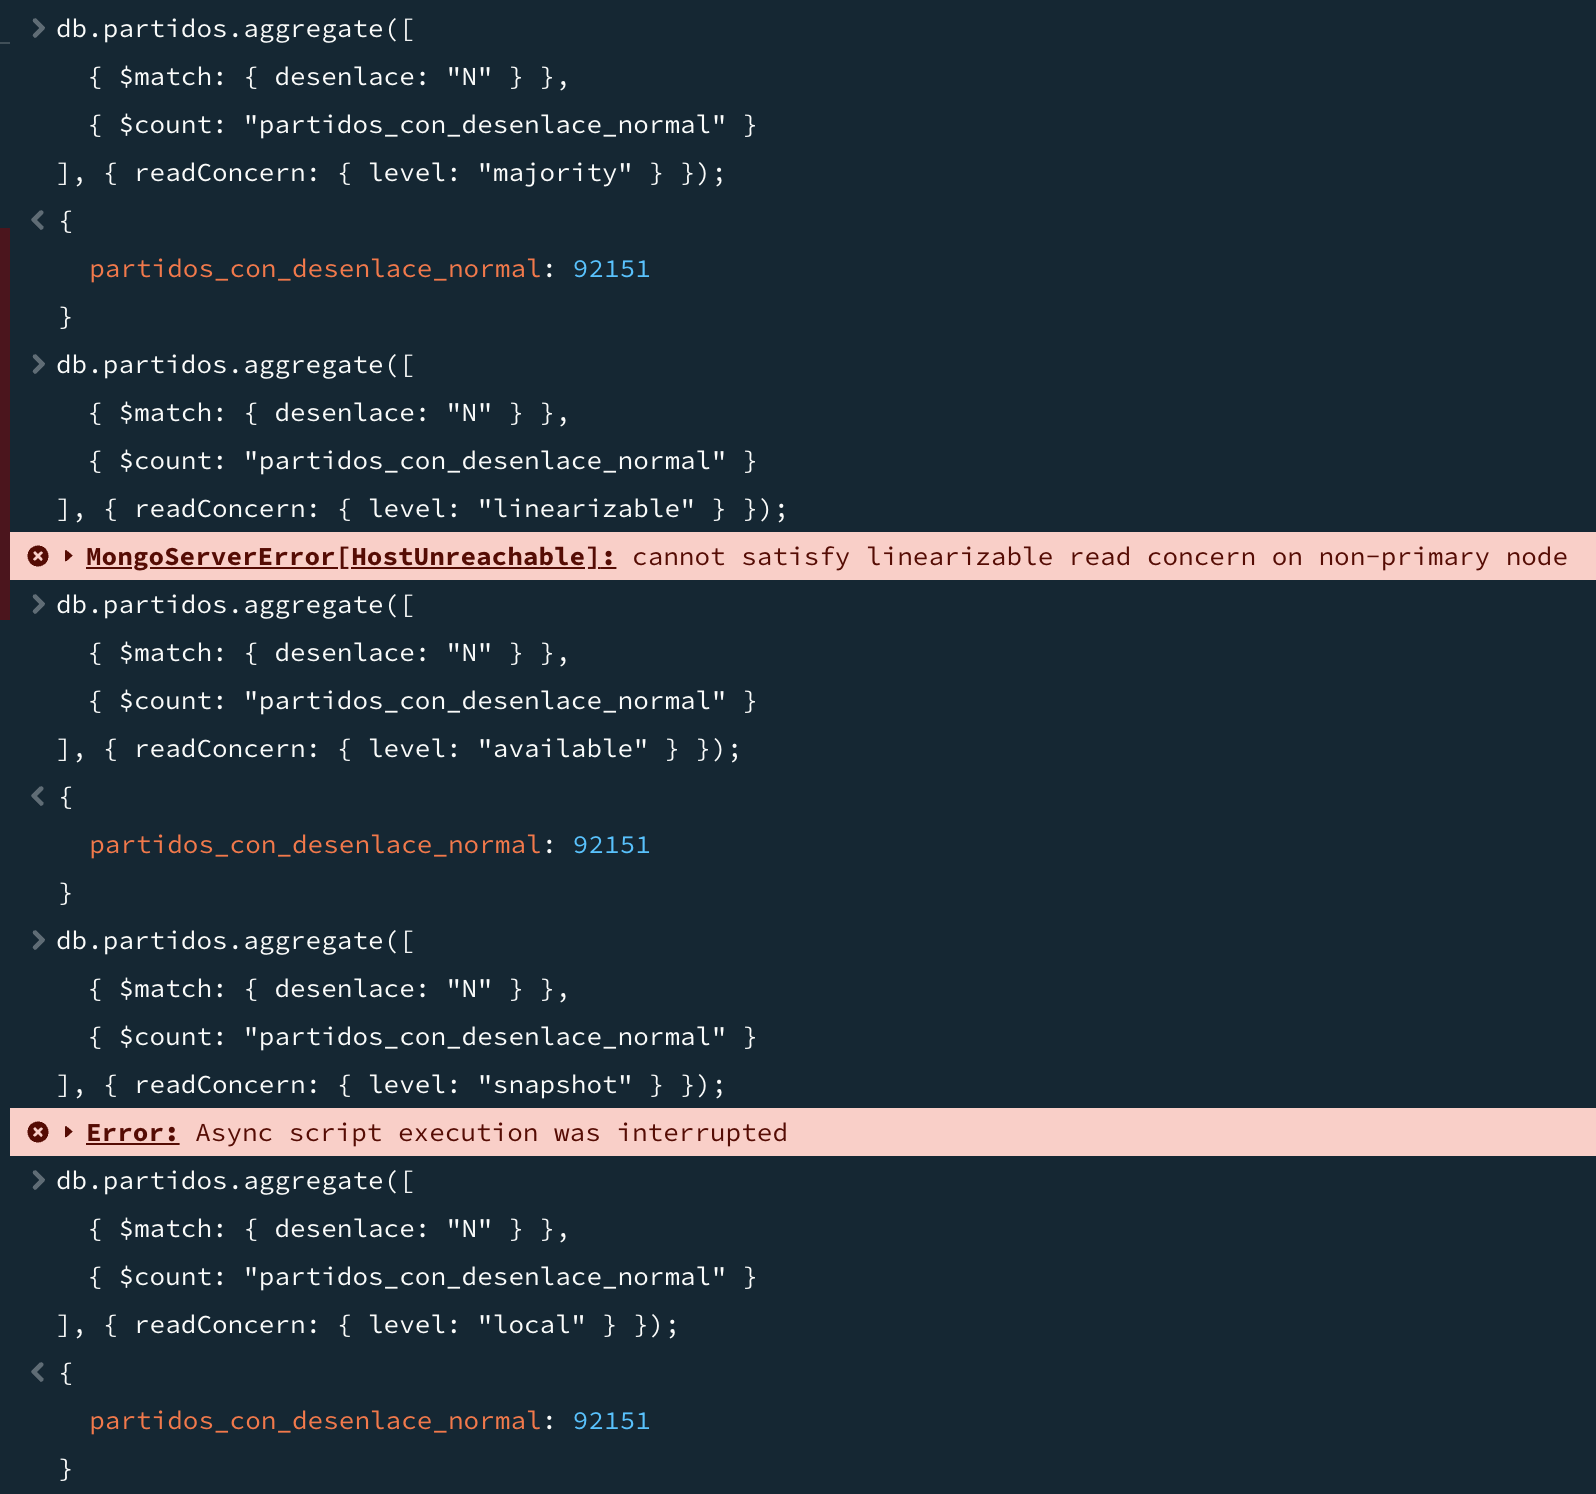
\includegraphics[width=0.55\textwidth]{fotos/mongo/read_concerns.png}
\caption{Efecto del compromiso de lectura al ejecutar la consulta.}
\label{fig:mongo_concerns}
\end{figure}

El compromiso de lectura \texttt{linearizable}, que nos garantiza leer los datos más recientes, falla, ya que este solo puede especificarse para operaciones de lectura desde el primario. También falla el compromiso de lectura \texttt{snapshot}, que requiere confirmar que los datos están en un estado consistente, cosa imposible con un solo nodo secundario, dado que no existe el \textit{quorum} necesario para garantizar esta consistencia.

\section{Bases de datos NoSQL: Grafos (Neo4j)}

\subsection{Creación de índices}

\begin{lstlisting}[language=Cypher]
CREATE INDEX IF NOT EXISTS FOR (j:Jugador) ON (j.id);
CREATE INDEX IF NOT EXISTS FOR (et:EdicionTorneo) ON (et.torneo, et.fecha);
CREATE INDEX IF NOT EXISTS FOR (p:Partido) ON (p.num_partido, p.fecha);
CREATE INDEX IF NOT EXISTS FOR (p:Pais) ON (p.codigo_iso2);
CREATE INDEX IF NOT EXISTS FOR (t:Torneo) ON (t.id);
CREATE INDEX partido_fecha_num IF NOT EXISTS FOR (p:Partido) ON (p.num_partido, p.fecha);
\end{lstlisting}

\subsection{Carga de datos con JBDC}

\begin{lstlisting}[language=Cypher]
// cargamos los paises
WITH "jdbc:postgresql://localhost:5432/tenis?user=alumnogreibd&password=greibd2021" as url
CALL apoc.load.jdbc(url, "SELECT codigo_iso2, codigo_iso3, codigo_ioc, nombre FROM pais") YIELD row
CREATE (p:Pais {
codigo_iso2: row.codigo_iso2,
codigo_iso3: row.codigo_iso3,
codigo_ioc: row.codigo_ioc,
nombre: row.nombre
});

// cargamos los jugadores
WITH "jdbc:postgresql://localhost:5432/tenis?user=alumnogreibd&password=greibd2021" AS url
CALL apoc.load.jdbc(url, 
"SELECT id, nombre, apellido, diestro, fecha_nacimiento, pais, altura FROM jugador") YIELD row
MATCH (pa:Pais {codigo_iso2: row.pais})
CREATE (j:Jugador {
    id: row.id,
    nombre: row.nombre,
    apellido: row.apellido,
    diestro: row.diestro,
    fecha_nacimiento: row.fecha_nacimiento,
    altura: row.altura
})
CREATE (j)-[:REPRESENTA_A]->(pa);

// cargamos los torneos
WITH "jdbc:postgresql://localhost:5432/tenis?user=alumnogreibd&password=greibd2021" AS url
CALL apoc.load.jdbc(url,
"SELECT id, nombre, pais FROM torneo") YIELD row
CREATE (t:Torneo {
    id: row.id,
    nombre: row.nombre
})
WITH t, row
OPTIONAL MATCH (pa:Pais {codigo_iso2: row.pais})
WITH t, pa
WHERE pa IS NOT NULL
CREATE (t)-[:SE_CELEBRA_EN]->(pa);

// cargamos las ediciones de los torneos
WITH "jdbc:postgresql://localhost:5432/tenis?user=alumnogreibd&password=greibd2021" AS url
CALL apoc.load.jdbc(url,
"SELECT torneo, fecha, superficie, tamano, nivel FROM edicion_torneo") YIELD row
MATCH (t:Torneo {id: row.torneo})
CREATE (et:EdicionTorneo {
    fecha: row.fecha,
    superficie: row.superficie,
    tamano: row.tamano,
    nivel: row.nivel,
    torneo: row.torneo
})
CREATE (et)-[:EDICION_DE]->(t);

// cargamos los partidos
WITH "jdbc:postgresql://localhost:5432/tenis?user=alumnogreibd&password=greibd2021" AS url
CALL apoc.load.jdbc(url,
"SELECT p.torneo, p.fecha, p.num_partido, p.num_sets, p.ronda, p.desenlace,
p.ganador, p.perdedor,
p.num_aces_ganador, p.num_dob_faltas_ganador, p.num_ptos_servidos_ganador,
p.num_primeros_servicios_ganador, p.num_primeros_servicios_ganados_ganador,
p.num_segundos_servicios_ganados_ganador, p.num_juegos_servidos_ganador,
p.num_break_salvados_ganador, p.num_break_afrontados_ganador,
p.num_aces_perdedor, p.num_dob_faltas_perdedor, p.num_ptos_servidos_perdedor,
p.num_primeros_servicios_perdedor, p.num_primeros_servicios_ganados_perdedor,
p.num_segundos_servicios_ganados_perdedor, p.num_juegos_servidos_perdedor,
p.num_break_salvados_perdedor, p.num_break_afrontados_perdedor
FROM partido p
WHERE p.fecha IS NOT NULL AND p.torneo IS NOT NULL
ORDER BY p.fecha, p.torneo, p.num_partido
LIMIT 10000 OFFSET 0") YIELD row

// creamos el partido independientemente de las referencias
CREATE (p:Partido {
num_partido: row.num_partido,
fecha: row.fecha,
num_sets: row.num_sets,
ronda: row.ronda,
desenlace: row.desenlace,
torneo_id: row.torneo // Guardamos la referencia al torneo aunque no exista el nodo
})

// vinculamos con el torneo si existe
WITH p, row
OPTIONAL MATCH (t:Torneo {id: row.torneo})
WITH p, row, t
WHERE t IS NOT NULL
CREATE (p)-[:SE_JUEGA_EN]->(t)

// vinculamos con el ganador si existe
WITH p, row
OPTIONAL MATCH (ganador:Jugador {id: toInteger(row.ganador)})
WITH p, row, ganador
WHERE ganador IS NOT NULL
CREATE (p)-[:GANADO_POR {
num_aces: row.num_aces_ganador,
num_dob_faltas: row.num_dob_faltas_ganador,
num_ptos_servidos: row.num_ptos_servidos_ganador,
num_primeros_servicios: row.num_primeros_servicios_ganador,
num_primeros_servicios_ganados: row.num_primeros_servicios_ganados_ganador,
num_segundos_servicios_ganados: row.num_segundos_servicios_ganados_ganador,
num_juegos_servidos: row.num_juegos_servidos_ganador,
num_break_salvados: row.num_break_salvados_ganador,
num_break_afrontados: row.num_break_afrontados_ganador
}]->(ganador)

// vinculamos con el perdedor si existe
WITH p, row
OPTIONAL MATCH (perdedor:Jugador {id: toInteger(row.perdedor)})
WITH p, row, perdedor
WHERE perdedor IS NOT NULL
CREATE (p)-[:PERDIDO_POR {
num_aces: row.num_aces_perdedor,
num_dob_faltas: row.num_dob_faltas_perdedor,
num_ptos_servidos: row.num_ptos_servidos_perdedor,
num_primeros_servicios: row.num_primeros_servicios_perdedor,
num_primeros_servicios_ganados: row.num_primeros_servicios_ganados_perdedor,
num_segundos_servicios_ganados: row.num_segundos_servicios_ganados_perdedor,
num_juegos_servidos: row.num_juegos_servidos_perdedor,
num_break_salvados: row.num_break_salvados_perdedor,
num_break_afrontados: row.num_break_afrontados_perdedor
}]->(perdedor);

// cargamos los sets de los partidos
WITH "jdbc:postgresql://localhost:5432/tenis?user=alumnogreibd&password=greibd2021" AS url
CALL apoc.load.jdbc(url,
"SELECT * FROM sets_partido LIMIT 10000 OFFSET 0") YIELD row
OPTIONAL MATCH (p:Partido {num_partido: row.num_partido, fecha: row.fecha})
WITH row, p
WHERE p IS NOT NULL
CREATE (sp:SetPartido {
num_set: row.num_set,
juegos_ganador: row.juegos_ganador,
juegos_perdedor: row.juegos_perdedor,
puntos_tiebreak_perdedor: row.puntos_tiebreak_perdedor
})
CREATE (sp)-[:PERTENECE_A]->(p);
\end{lstlisting}

\subsubsection{Muestra todos los ganadores del torneo ``Wimbledon'' (Nombre apellidos y año). Ordena el resultado por año.}

\begin{lstlisting}[language=Cypher]
MATCH (j:Jugador)-[gp:GANADO_POR]-(p:Partido)-[:SE_JUEGA_EN]->(t:Torneo)
WHERE t.nombre = 'Wimbledon'
AND p.ronda = 'F'
RETURN j.nombre AS nombre,
j.apellido AS apellido,
substring(toString(p.fecha), 0, 4) AS ano
ORDER BY ano;
\end{lstlisting}





\subsubsection{Muestra los años en los que Roger Federer ganó algún torneo de nivel Gran Slam (G) o Master 1000 (M). Para cada año, muestra el número de torneos y lista sus nombres (ordenados por la fecha de celebración). Ordena el resultado por el año}

\begin{lstlisting}[language=Cypher]
MATCH (j:Jugador)-[:GANADO_POR]-(p:Partido)-[:SE_JUEGA_EN]->(t:Torneo)
MATCH (et:EdicionTorneo)-[:EDICION_DE]->(t)
WHERE j.nombre = 'Roger'
AND j.apellido = 'Federer'
AND p.ronda = 'F'
AND et.nivel IN ['G', 'M']
AND et.fecha = p.fecha
AND et.torneo = t.id
WITH substring(toString(p.fecha), 0, 4) AS ano,
collect(DISTINCT t.nombre) AS torneos_nombres,
count(DISTINCT t) AS num_torneos
RETURN ano,
num_torneos,
reduce(s = head(torneos_nombres), x IN tail(torneos_nombres) | s + ', ' + x) AS torneos
ORDER BY ano;
\end{lstlisting}





\subsubsection{Muestra los partidos de semifinales (ronda='SF') y final (ronda = 'F') del torneo de "Roland Garros" del 2018. Para cada partido muestra la ronda, el tipo de desenlace, el nombre y apellidos del ganador y el nombre y apellidos del perdedor y el resultado con el número de juegos del ganador y del perdedor en cada set, y opcionalmente en paréntesis el número de juegos del perdedor en el tie break}

\begin{lstlisting}[language=Cypher]
MATCH (jg:Jugador)-[:GANADO_POR]-(p:Partido)-[:PERDIDO_POR]-(jp:Jugador),
(p)-[:SE_JUEGA_EN]->(t:Torneo),
(sp:SetPartido)-[:PERTENECE_A]->(p)
WHERE t.nombre = 'Roland Garros'
AND p.ronda IN ['SF', 'F']
AND substring(toString(p.fecha), 0, 4) = '2018'
WITH p, jg, jp, sp
ORDER BY sp.num_set
WITH p, jg, jp,
collect(sp.juegos_ganador + '-' + sp.juegos_perdedor +
CASE sp.puntos_tiebreak_perdedor
WHEN null THEN ''
ELSE '(' + toString(sp.puntos_tiebreak_perdedor) + ')'
END) as sets
RETURN p.ronda as ronda,
p.desenlace as desenlace,
jg.nombre + ' ' + jg.apellido as ganador,
jp.nombre + ' ' + jp.apellido as perdedor,
reduce(s = head(sets), x IN tail(sets) | s + ', ' + x) as resultado
ORDER BY p.fecha;
\end{lstlisting}





\subsubsection{Muestra la lista de jugadores españoles (ES) que ganaron algún torneo de nivel Gran Slam (G). Para cada jugador muestra los siguientes datos resumen de todos sus partidos: número de partidos jugados, porcentaje de victorias, porcentaje de aces, porcentaje de dobles faltas, porcentaje de servicios ganados, porcentaje de restos ganados, porcentaje de break points salvados (de los sufridos en contra), porcentaje de break points ganados (de los provocados a favor)}

\begin{lstlisting}[language=Cypher]
// Primero identificamos los jugadores espanoles que han ganado finales de Grand Slam
MATCH (j:Jugador)-[:REPRESENTA_A]->(p:Pais {codigo_iso2: 'ES'})
MATCH (j)-[:GANADO_POR]-(partido:Partido)-[:SE_JUEGA_EN]->(t:Torneo)
MATCH (et:EdicionTorneo)-[:EDICION_DE]->(t)
WHERE partido.ronda = 'F'
AND et.nivel = 'G'
AND et.fecha = partido.fecha
AND et.torneo = t.id
WITH DISTINCT j.id as id_jugador, j.nombre + ' ' + j.apellido as jugador


// Ahora calculamos todas las estadisticas para estos jugadores
MATCH (j:Jugador)
WHERE j.id = id_jugador
MATCH (p:Partido)
MATCH (j)-[r:GANADO_POR|PERDIDO_POR]-(p)
WITH jugador, p, j, r, type(r) as tipo,
CASE type(r) WHEN 'GANADO_POR' THEN 1 ELSE 0 END as es_ganador,
CASE type(r)
WHEN 'GANADO_POR' THEN r.num_aces
ELSE r.num_aces END as aces,
CASE type(r)
WHEN 'GANADO_POR' THEN r.num_ptos_servidos
ELSE r.num_ptos_servidos END as ptos_servidos,
CASE type(r)
WHEN 'GANADO_POR' THEN r.num_dob_faltas
ELSE r.num_dob_faltas END as dobles_faltas,
CASE type(r)
WHEN 'GANADO_POR' THEN r.num_primeros_servicios_ganados + r.num_segundos_servicios_ganados
ELSE r.num_primeros_servicios_ganados + r.num_segundos_servicios_ganados END as servicios_ganados,
// Para restos ganados necesitamos el rival
CASE type(r)
WHEN 'GANADO_POR' THEN [(p)-[rp:PERDIDO_POR]-() | rp.num_ptos_servidos - rp.num_primeros_servicios_ganados - rp.num_segundos_servicios_ganados][0]
ELSE [(p)-[rg:GANADO_POR]-() | rg.num_ptos_servidos - rg.num_primeros_servicios_ganados - rg.num_segundos_servicios_ganados][0] END as restos_ganados,
CASE type(r)
WHEN 'GANADO_POR' THEN [(p)-[rp:PERDIDO_POR]-() | rp.num_ptos_servidos][0]
ELSE [(p)-[rg:GANADO_POR]-() | rg.num_ptos_servidos][0] END as ptos_servidos_rival,
CASE type(r)
WHEN 'GANADO_POR' THEN r.num_break_salvados
ELSE r.num_break_salvados END as breaks_salvados,
CASE type(r)
WHEN 'GANADO_POR' THEN r.num_break_afrontados
ELSE r.num_break_afrontados END as breaks_afrontados,
CASE type(r)
WHEN 'GANADO_POR' THEN [(p)-[rp:PERDIDO_POR]-() | rp.num_break_afrontados - rp.num_break_salvados][0]
ELSE [(p)-[rg:GANADO_POR]-() | rg.num_break_afrontados - rg.num_break_salvados][0] END as breaks_ganados,
CASE type(r)
WHEN 'GANADO_POR' THEN [(p)-[rp:PERDIDO_POR]-() | rp.num_break_afrontados][0]
ELSE [(p)-[rg:GANADO_POR]-() | rg.num_break_afrontados][0] END as breaks_rival
WITH jugador,
count(p) as partidos,
100.0 * sum(es_ganador) / count(p) as pcje_victorias,
CASE WHEN sum(ptos_servidos) = 0 THEN 0
ELSE 100.0 * sum(aces) / sum(ptos_servidos) END as pcje_aces,
CASE WHEN sum(ptos_servidos) = 0 THEN 0
ELSE 100.0 * sum(dobles_faltas) / sum(ptos_servidos) END as pcje_dobles_faltas,
CASE WHEN sum(ptos_servidos) = 0 THEN 0
ELSE 100.0 * sum(servicios_ganados) / sum(ptos_servidos) END as pcje_servicios_ganados,
CASE WHEN sum(ptos_servidos_rival) = 0 THEN 0
ELSE 100.0 * sum(restos_ganados) / sum(ptos_servidos_rival) END as pcje_restos_ganados,
CASE WHEN sum(breaks_afrontados) = 0 THEN 0
ELSE 100.0 * sum(breaks_salvados) / sum(breaks_afrontados) END as pcje_breaks_salvados,
CASE WHEN sum(breaks_rival) = 0 THEN 0
ELSE 100.0 * sum(breaks_ganados) / sum(breaks_rival) END as pcje_breaks_ganados
RETURN
jugador,
partidos,
round(pcje_victorias, 1) as pcje_victorias,
round(pcje_aces, 1) as pcje_aces,
round(pcje_dobles_faltas, 1) as pcje_dobles_faltas,
round(pcje_servicios_ganados, 1) as pcje_servicios_ganados,
round(pcje_restos_ganados, 1) as pcje_restos_ganados,
round(pcje_breaks_salvados, 1) as pcje_breaks_salvados,
round(pcje_breaks_ganados, 1) as pcje_breaks_ganados
ORDER BY jugador;
\end{lstlisting}





\subsubsection{Lista los jugadores que fueron derrotados (en algún partido del 2018) por el rival de Rafael Nadal de la primera ronda (R128) de Roland Garros de 2018}

\begin{lstlisting}[language=Cypher]
// Primero encontramos al rival de Nadal en Roland Garros 2018 R128
MATCH (nadal:Jugador {nombre: 'Rafael', apellido: 'Nadal'})
MATCH (rival:Jugador)
MATCH (p:Partido)-[:SE_JUEGA_EN]->(t:Torneo {nombre: 'Roland Garros'})
WHERE p.ronda = 'R128'
AND substring(toString(p.fecha), 0, 4) = '2018'
AND ((nadal)-[:GANADO_POR]-(p)-[:PERDIDO_POR]-(rival) OR
(nadal)-[:PERDIDO_POR]-(p)-[:GANADO_POR]-(rival))


// Ahora buscamos los partidos donde este rival perdio en 2018
WITH rival
MATCH (rival)-[:GANADO_POR]-(derrotas:Partido)-[:PERDIDO_POR]-(perdedor:Jugador)
WHERE substring(toString(derrotas.fecha), 0, 4) = '2018'
MATCH (perdedor)-[:REPRESENTA_A]->(pais:Pais)
RETURN DISTINCT
perdedor.nombre + ' ' + perdedor.apellido as jugador,
pais.codigo_iso2 as pais
ORDER BY jugador;
\end{lstlisting}
    
    


\end{document}
